%%%%%%%%%%%%%%%%%%%%%%%%%%%%%%%%%%%%%%%%%%%%%%%%%%%%%%%%

%%%  Welcome to the Cell Press LaTeX template,
%%%  version 1.10. This is a minimalist template
%%%  to help you organize your article for
%%%  publication at Cell Press. PLEASE NOTE:

%%%  (1) If you submit your final manuscript materials
%%%  in LaTeX format, our typesetters will prepare
%%%  a Word file for use in production. This conversion
%%%  process allows us to copyedit your paper, fix
%%%  any typos, and add formatting and tagging. The
%%%  conversion process will add approximately 3
%%%  business days to the production timeline.
%%%  Authors using LaTeX should keep this in mind
%%%  when considering deadlines.

%%%  (2) Keep your LaTeX files as simple as possible.
%%%  Avoid the use of elaborate local macros and/or
%%%  customized external style files. If you need
%%%  additional macros, please keep them simple and
%%%  include them in the actual .tex document preamble.
%%%  Source code should be set up so that all .sty
%%%  and .bst files called by the main .tex file are
%%%  in the same directory as the main .tex file.

%%%  (3) Cell Press publishes more than 40 journals,
%%%  some of which may have different or additional
%%%  formatting requirements not specified in this
%%%  template. When revising your paper before
%%%  acceptance, please review the formatting
%%%  guidelines, including the Final Files Requirements,
%%%  for the journal you are publishing with.

%%%  Please send feedback on this template to lshipp@cell.com.

%%%%%%%%%%%%%%%%%%%%%%%%%%%%%%%%%%%%%%%%%%%%%%%%%%%%%%%%

\documentclass[12pt,letterpaper]{article}
\usepackage[a4paper, total={7in, 10in}]{geometry}
\renewcommand{\familydefault}{\sfdefault}
\usepackage{graphicx}
\usepackage{helvet}
\usepackage{authblk}
\usepackage{hyperref}
\usepackage{booktabs}
\usepackage{tabularx}
\usepackage{amsmath}
\usepackage{amssymb}
\usepackage{orcidlink}
\usepackage[super,comma,sort&compress]
   {natbib}\bibliographystyle{numbered}
\usepackage[right]{lineno} \linenumbers

\graphicspath{ {../figures/} }

\makeatletter
\renewcommand{\maketitle}{\bgroup\setlength{\parindent}{0pt}
\begin{flushleft}
  \textbf{\@title}

  \@author
\end{flushleft}\egroup}
\makeatother

%%%  Insert title below; leave date empty.

\title{Inferring the Recombinant Genealogy of a Pandemic Pathogen in Real Time}
\date{}

%%%  Author first and last names should be spelled
%%%  out in their entirety (do not abbreviate "J.H.
%%%  Watson" unless this is how the author's name
%%%  always appears). Middle initials are OK. Do
%%%  not include titles, positions, or degrees.

%%%  Use numbered footnotes to indicate institutional
%%%  affiliations. Authors may have multiple
%%%  institutional affiliations, and affiliations
%%%  may be shared among multiple authors.

%%%  After the institutional affiliations, numbered
%%%  footnotes may be used to indicate an author's
%%%  present address, equal contribution status,
%%%  and/or senior author status.

%%%  The final numbered footnote should indicate
%%%  which author is the lead contact (required).
%%%  One author must be designated as the lead contact.
%%%  There can be no more than one lead contact.

%%%  Corresponding authors should be indicated with
%%%  asterisks (*). Use 2 asterisks (**) for the
%%%  second-listed corresponding author, 3 (***) for
%%%  the third-listed, and so on. The lead contact
%%%  must be a corresponding author. Additional
%%%  authors may also serve as corresponding authors.

\author[1,\orcidlink{0000-0000-0000-0000}]{First Last}
\author[1,2]{First Middle Last}
\author[2,3]{First M.M. Last}
\author[3,*]{First Last, Jr.}
\author[3,4,5,**]{F. Middle Last}


%%%  Institutional affiliations should contain the
%%%  following information at minimum: department(s)/
%%%  subunit(s), institution, city, state/region (if
%%%  applicable), and country.

\affil[1]{University A, London SW7 2AZ, UK}
\affil[2]{Department B, University B, Toronto, ON M5S 3H6, Canada}
\affil[3]{Division C, Department C, University C, Cambridge, MA, USA}

\affil[4]{Senior author}
\affil[5]{Lead contact}

%%%  List only one email address per corresponding author.

\affil[*]{Correspondence: first.last.jr@university.edu}
\affil[**]{Correspondence: f.middle.last@university.edu}


\begin{document}

\maketitle

%%% The summary (abstract) should consist of a single paragraph of 150 words or
%%% fewer.

\section*{SUMMARY}

% NOTE: currently 160 words

Millions of SARS-CoV-2 genome sequences were collected in
response to the COVID-19 pandemic, forming a dataset of unprecedented
depth and richness.
Estimated genealogies are fundamental to
gleaning information from this ocean of data, 
and form the primary input to many downstream analyses.
A basic assumption of methods to infer genealogies from viral 
genetic sequence data is that recombination is negligible and 
the genealogy is a tree.
Recombinant lineages have risen to global prevalence in SARS-CoV-2,
and therefore such single-tree representations are necessarily
incomplete and potentially misleading.
We present sc2ts, a method to infer reticulate genealogies for SARS-CoV-2
that automatically detects and incorporates recombination 
in real time.  
We use sc2ts to infer a genealogy of 2.48 million genomes,
and show that it captures a broad range of 
known evolutionary features and provides novel 
insights into the relationships between previously identified
recombinant lineages.
Together, the inference method, inferred genealogy and 
suite of open-source analysis tools, 
represent a powerful resource for future research.


\section*{KEYWORDS}

%%%  Include up to 10 keywords, separated by commas.
%%%  Keywords entered in EM are not carried over; only
%%%  keywords included in the main text will be used
%%%  in the final article metadata. Please note that
%%%  for some journals, keywords are chosen by the editors.

Ancestral recombination graphs, population genetics, recombination, tree sequence, SARS-CoV-2


\section*{INTRODUCTION}

%%% No subheadings, please. Use of abbreviations should be kept to a minimum,
%%% and nonstandard abbreviations should be defined when first used in the text.

The genomic revolution has transformed how we study the evolution and spread of pathogens,
allowing real-time tracking of pathogens over time and space.
During the COVID-19 pandemic, thousands of SARS-CoV-2 genome sequences were generated daily,
quickly overwhelming typical phylogenetic approaches.
Although real-time phylogenetic methods now exist to cope with this flood of genomic data
(e.g., UShER \cite{Turakhia2021} and MAPLE \cite{DeMaio2023}),
we lack methods to build phylogenies that can integrate recombination
in the face of ongoing sampling of infected cases.

UShER is a maximum parsimony method developed during the pandemic to infer phylogenies
from large numbers of densely sampled SARS-CoV-2 genome sequences \cite{Turakhia2021}.
UShER has generated phylogenies updated daily \cite{McBroome2021} and
has proven to be a powerful resource that successfully enabled the world
to keep up with an evolving disease (e.g., through the Nextstrain web portal \cite{Hadfield2018}).
These phylogenies are used to identify and monitor
potentially epidemiologically important ``Pango'' lineages \cite{Rambaut2020,McBroome2024},
which might have acquired features to become Variants of Concern (VOC),
for example, increased transmissibility, disease severity, and immune escape.
Beyond supporting real-time genomic epidemiology,
UShER phylogenies have been used in a multitude of evolutionary and epidemiological studies of SARS-CoV-2
(e.g., \cite{Karthikeyan2022,Obermeyer2022,Turakhia2022,Bloom2023}).
UShER uses a tree to represent evolutionary change via mutation,
assuming no recombination \cite{Turakhia2021}.
However, given extensive evidence for recombination in SARS-CoV-2
\cite{Jackson2021,VanInsberghe2021,Focosi2022,Gutierrez2022,Ignatieva2022,Tamura2023},
the tree-like representation of UShER is no longer tenable.

Ancestral Recombination Graphs (ARGs) are reticulate genealogies
that incorporate both mutation and recombination events \cite{Wong2024},
potentially allowing more comprehensive evolutionary representations of SARS-CoV-2
and other viruses undergoing recombination.
Until recently, ARGs lacked software support and
sufficiently scalable inference methods to be of practical use.
Recent advances enable ARG inference for tens to hundreds of thousands of human genomes \cite{Kelleher2019,Speidel2019,Zhang2023},
with high levels of recombination.
These advances now enable evolutionary genealogies to be built quickly and at scale, and
there is a surge of excitement in the inference and applications of ARGs \cite{Brandt2024,Lewanski2024,Wong2024,Nielsen2025}.

Previous ARG methods are retrospective \cite{Rasmussen2014,Kelleher2019,Speidel2019,Ignatieva2022,Zhang2023},
reconstructing the past from a sample of genome sequences drawn at one moment in time,
but scientists are increasingly tracking evolutionary change as it happens,
accumulating data forward in time.
For example, sequences from daily samples of SARS-CoV-2 were made globally available on a daily basis,
leading to over 17 million sequences in the GISAID database \cite{Shu2017}.

Here, we present
(1) sc2ts, a new method to infer ARGs in real time by building genealogies forward in time, and
(2) an ARG for SARS-CoV-2 with ~2.48 million genome sequences.
We used the ``Viridian'' dataset,
which is purged of various systematic errors and artifacts \cite{Hunt2024} and
show that this ARG is highly congruent to an UShER phylogeny built from the same dataset.
Compared to previously identified recombinants,
we show that this ARG contains the vast majority of epidemiologically relevant signals of recombination,
while adding significant nuance and texture.
This ARG – which captures the major signals of evolution
through phylogenetic relationships, point mutations, deletions, and recombination –
is a resource of unprecedented detail and precision, and
should provide a strong basis for future studies of SARS-CoV-2.


\section*{RESULTS}

%%% The results may be divided with subheadings.
%%% In our view, good subheadings convey information about the findings,
%%% so we encourage you to be specific. For example, "Factor X requires factor Y to function in process Z"
%%% is better than "Analysis of factors X and Y by approach Q."
%%% We recommend that you use similar language in your figure titles for clarity and structural harmony.
%%% Please do not use numbered subheadings. For some formats, ``results and discussion" may be combined under a single heading.

%%% For initial submissions, figures and their titles and legends can be run-in with the text.
%%% For final submissions, the image files must be uploaded as separate files, one complete file per figure. The figure titles and legends should be placed toward the end of the main text, after the declaration of interests. Our typesetters will place the figures and their titles and legends appropriately based on your in-text citations.

%%% To cite/link to display items (figures and tables) and/or sections of the manuscript,
%%% simply write, for example, ``(Figure 1)" or ``see discussion."
%%% Our team will do the rest. Please note that we do not number sections or subsections.

\subsection*{Brief description of sc2ts}

Sc2ts reconstructs an ARG by incrementally adding batches of sequences as they become available
(Figure~\ref{fig:methodology}; for details, see STAR Methods).
First, sc2ts infers likely ``copying paths'' connecting each sample in the batch to node(s) in the current ARG
(allowing recombination) using the Li and Stephens (LS) model \cite{LiStephens2003},
which is a Hidden Markov Model (HMM) widely used in human genomics
to approximate the effects of mutation and recombination on genetic inheritance.
As recombination is relatively rare in viruses,
we would expect most samples to copy from a single parent in the ARG.
Recombinant samples, however, copy from two or more parents, with switching (recombination) in the copying path
between the parents resulting in different genomic segments inherited from the different parents.
Next, for clusters within the batch that are inferred to copy from the same ARG node,
sc2ts uses standard phylogenetic techniques to resolve relationships within the cluster.
Finally, sc2ts attaches the phylogenies of the clusters to the current ARG, and
applies parsimony-improving heuristics to address issues introduced by the inherent greediness of this strategy.
[TODO add brief summary of sample filtering and how we handle VOCs, 
refing Methods for details]

\begin{figure}[h]
\centering
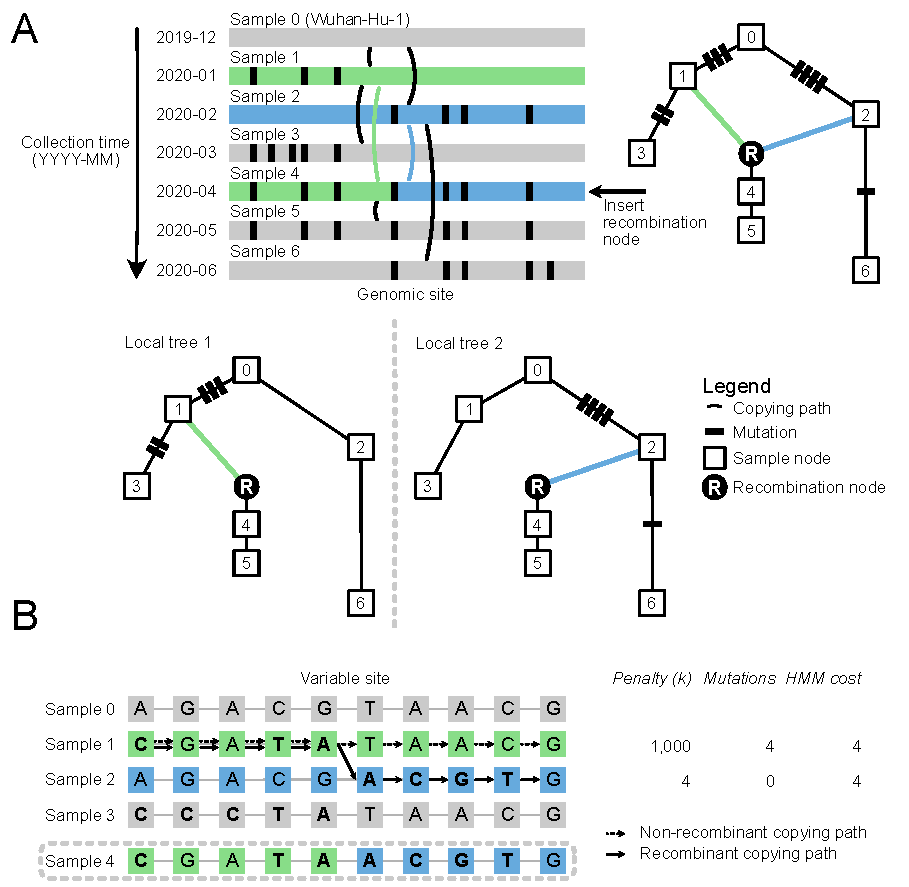
\includegraphics[width=0.85\linewidth]{sc2ts_methodology}
\caption{
Schematic overview of sc2ts.
(A) Process to build an ARG by incrementally updating it with samples sorted by collection dates.
(B) The ARG resulting from the inference process.
Sample 0 is used to initialize the ARG as the root.
Next, Sample 1 is attached, mapping mutations onto the new branch to explain it.
When Sample 4 is detected as a recombinant,
a node representing the recombination event is inserted with two edges connecting to its parents,
with Sample 4 itself attached to this node as its child.
(C) Two local trees contained in the resulting ARG,
one on each side of the inferred breakpoint (A), which occurs at position 50.
The genomic coordinates of the segments inherited from different recombinant parents
are denoted by two half-open intervals (B).
(D) Copying paths for Sample 4 inferred under the LS model
while allowing recombination ($k = 4$) or disallowing it ($k = 1000$).
}
\label{fig:methodology}
\end{figure}

%% JK: This is copy of old Methods section "overview of sc2ts" which is basically
%% the same as this section. TODO Merge the useful text in here.

% Sc2ts (pronounced ``scoots'', optionally)
% is a method for inferring Ancestral Recombination Graphs (ARGs)
% from densely sampled genome sequence data in real time,
% in which recombination occurs at a low but significant rate.
% The basic idea is to incrementally update an ARG regularly
% with the sequences collected since the previous batch (Figure
% \ref{fig:methodology}).
% We used daily batches for SARS-CoV-2,
% and use days as the time interval for clarity in what follows.
% The first step is to find likely ``copying paths'' under the Li and Stephens (LS) model \cite{LiStephens2003}
% for each sequence in the daily batch to the current ARG.
% These copying paths will mostly consist of a new sample sequence copying
% from a node in the ARG with a small number of mutations,
% and often many samples from a daily batch will copy from the same ARG node.
% The second step is then to ``resolve'' these implied polytomies
% by using a standard neighbor-joining algorithm \cite{Saitou1987}.
% This greedy update strategy inevitably leads to unparsimonious topologies,
% and the third step is to then increase the overall parsimony of the inferred ARG
% by making some simple topological updates.
% Recombination is inferred as an integral and ongoing part of this process,
% requiring only a few additional steps to facilitate later analysis.
% The result of inference for a given day is then a genealogy recording genetic inheritance
% as well as mutation and recombination events
% for all of the samples added to the ARG up to that day.

% Sc2ts is implemented in Python building on core PyData infrastructure
% such as Numpy\cite{Harris2020array}, SciPy\cite{Virtanen2020scipy}
% and Pandas~\cite{Mckinney2010data} ,
% using pyfaidx\cite{Shirley2015efficient} to access alignment data
% and Numba~\cite{Lam2015numba} to accelerate certain alignment processing
% tasks.
% [TODO JK to fill this out]

\subsection*{A comprehensive representation of SARS-CoV-2 evolution}

Using sc2ts, we built an ARG of $\sim$2.48 million samples spanning the COVID-19 pandemic.
Inference took 21 days on a server equipped with dual EPYC (details) and 500 GB of RAM 
(~5 CPU years; Figure~\ref{fig:inference_resources}).
The ARG contains 2,689,054 nodes representing the genealogical relationships
among 2,482,157 sampled genomes in the Viridian v04 dataset,
which were collected from January 01, 2020 to February 20, 2023 \cite{Hunt2024}.
Of the nodes, 855 represent recombination events,
of which 356 have a minimum of four loci supporting the non-focal parent on both sides of the breakpoint
(we refer to these as ``robust'' recombination events,
Figure~\ref{fig:recombinant_qc}; see STAR Methods)
reflecting the overwhelmingly tree-like structure of SARS-CoV-2 evolutionary history.

The ARG represents the full evolutionary history of SARS-CoV-2 and 
is in close agreement with a state-of-the-art UShER phylogeny built using the Viridian dataset \cite{Hunt2024}.
First, we validated the broad structure of the ARG against the UShER phylogeny \cite{Hunt2024}
by pruning both down to representative samples for 1097 deeply-sampled 
lineages (STAR Methods).
Tanglegrams show that the ARG closely matches the phylogenetic
structure of the UShER tree (Figures~\ref{fig:tanglegram_base},
\ref{fig:tanglegram_delta},
\ref{fig:tanglegram_ba2},
\ref{fig:tanglegram_ba5}).
Next, we compared the sc2ts and UShER inferences 
from the Viridian dataset
by pruning both to their intersection of 2,475,418 samples and 27,507 sites,
% JK: this feels a bit wishy washy, but there really is no simple answer to
% this and I don't want to claim we're more parsimonious.
and found they were very similar in terms of parsimony
(Document~\ref{sec:supplement_sc2ts_usher_parsimony})
and imputation of missing and ambiguous bases
(Document~\ref{sec:supplement_sc2ts_usher_imputation}).
We also compared the mutational spectra of major VOCs in the ARG against 
the mutational spectra 
from the Viridian UShER phylogeny \cite{Hunt2024} and a previous study \cite{Bloom2023} (STAR Methods),
finding a close match to them (Figure~\ref{fig:mutational_spectra}).

Input genome alignments are masked in sc2ts
so that deletions and ambiguous bases are treated as missing data by the HMM,
and once the samples are incorporated into the ARG,
these bases are imputed to carry the values inherited by the node in question.
Deletions are an important part of SARS-CoV-2 evolution \cite{Jeronimo2023}, however,
and to incorporate them into the ARG we identified a set of [XXX] sites
most frequently involved in deletions [cite source?]
and post-hoc mapped alignment data for these sites to the ARG using parsimony.
Although sites are treated independently in this approach,
the approximation successfully identified the most frequent deletions,
such as the recurrent 21991-21993 (See Document~\ref{sec:supplement_dels}
for additional analysis).
The node representing the origin of Alpha, with 290,407 descendants,
is correctly associated with key lineage-defining deletions:
11288-11296 (ORF1A del3675-3677),
21765-21770 (Spike del69-70),
21991-21993 (Spike del144), and
28271 (non-coding).
The Spike 69-70 deletion, which causes S-Gene Target Failure \cite{Walker2021},
also emerges twice in the origin of Omicron -
in the node leading to the BA.1 variant (342,099 descendants),
and the node leading to the BA.4 variant (189,746 descendants).
To speed up inference and to avoid issues caused by sites enriched for errors [citation?],
sc2ts masks out a set of 100 sites identified as the most highly homoplasic
by running on a subset of the data (STAR Methods).
Of these sites, 9 are in the set of [1XX] ``problematic sites'' 
masked by UShER \cite{Hunt2024}.
In addition to remapping the data for sites identified as being involved in deletions,
we added mutations for XX of these highly recurrent sites
that are used in Pango designation \cite{Rambaut2020} by post-hoc parsimony.
Each node in the ARG was then assigned to one of 2058 Pango lineages using pangolin (STAR Methods).
All but 21,680 sampled sequences (0.87\%) agreed with the source sequences in terms of Pango lineage assignment
(comparable to the 0.27\% disagreement between pangolin-data 
versions 1.21 and 1.29 in the source Viridian metadata).
A majority of these lineages (1473 of 2058) have monophyletic origins within the ARG,
increasing to 1779 (86\%) when we allow for multiple sibling origination 
nodes (Document~\ref{sec:supplement_pango_lineages}).

\subsection*{Epidemiologically relevant recombinant lineages}

As new data became available during the pandemic,
volunteers continually detected recombinants which might have concerning features,
particularly increased transmissibility, disease severity, and
ability to escape natural or vaccine-induced immunity (e.g., \cite{Tamura2023}).
The process of gathering evidence for and characterizing such recombinants is manual,
involving visual inspection of phylogenies for unusual branches
caused by forcibly placing recombinant sequences onto them,
typically followed by visual analysis of genome sequence alignments
to identify parental lineages and breakpoint locations.
This process has resulted in the designation of recombinant Pango lineages
(whose aliases begin with an ''X'', e.g., XA and XBB).

We find strong evidence for the recombination events leading to 17 Pango X lineages
in the ARG (Table~\ref{tab:pango_x_lineages}),
all of which pass the robustness filtering criteria (Figure~\ref{fig:recombinant_qc}).
%% JK: Does saying this here help at all? I think we may be better off without 
% These events are supported by high numbers of averted
% mutations (Table 1) and high numbers of loci matching their suggested parents
% (see their copying patterns in Figure SX). 
Among these Pango X lineages are XA,
which is the first designated Pango X lineage that
showed signs of onward transmission \cite{Jackson2021}, and
XBB, which escaped vaccine-induced immunity and gained global prevalence \cite{Tamura2023}.
The recombinant origin of XA is well explained in the ARG by two parents and one mutation
(Figure~\ref{fig:subgraphs}A; Table~\ref{tab:pango_x_lineages}), 
with sc2ts correctly identifying its parental Pango lineages and breakpoint location.

Furthermore, some of the Pango X lineages above originate from
shared recombination events in the ARG (Table~\ref{tab:pango_x_lineages}).
An example of a set of ``nested'' closely related lineages consists of XZ, XAC, XAD, XAE, and XAP,
which descend from a single recombination event rather than five independent
events in the ARG (Figure~\ref{fig:subgraphs}B).
These Pango X lineages were designated around the same time.
These results highlight that the ARG can help clarify the relationships between recombinants,
allowing more precise interpretation of evidence for recombination.

Sc2ts identified 12 Pango X lineages in the ARG as non-recombinants
(Table~\ref{tab:pango_x_lineages}), on the basis of the HMM and available data.
For all these Pango X lineages, the number of recombination-informative sites
fell below our threshold of detection (i.e. $k = 4$ in the HMM).
The fact that most of these Pango X lineages (except XAJ and XAN) differ from a single parent node in the ARG
by at most three mutations (Table~\ref{tab:pango_x_lineages}) strongly supports 
their origins as non-recombinants.
For example, the closely related XN and XAU can be explained by two mutations
and one mutation in the ARG, respectively (Figure~\ref{fig:subgraphs}C).
%%% TODO: Say something about XAJ and XAN.
%JK: we should weaken this statement a bit, as we're not certain that they 
% really are recombinants, especially XP.
However, sc2ts did not detect several Pango X lineages (XB, XP, and XAJ) as recombinants
because the HMM treated characteristic deletions as missing data.


[NOTE: putting this here for now, until we find the right place to slot it
in next draft.]
See Document~\ref{sec:supplement_indepth_pango_x_lineages} for extended analyses,
Figure~\ref{fig:pango_x_copying_patterns} for copying patterns,
and Document S2 for ARG visualations of all Pango X lineages.

\begin{figure}[h]
\centering
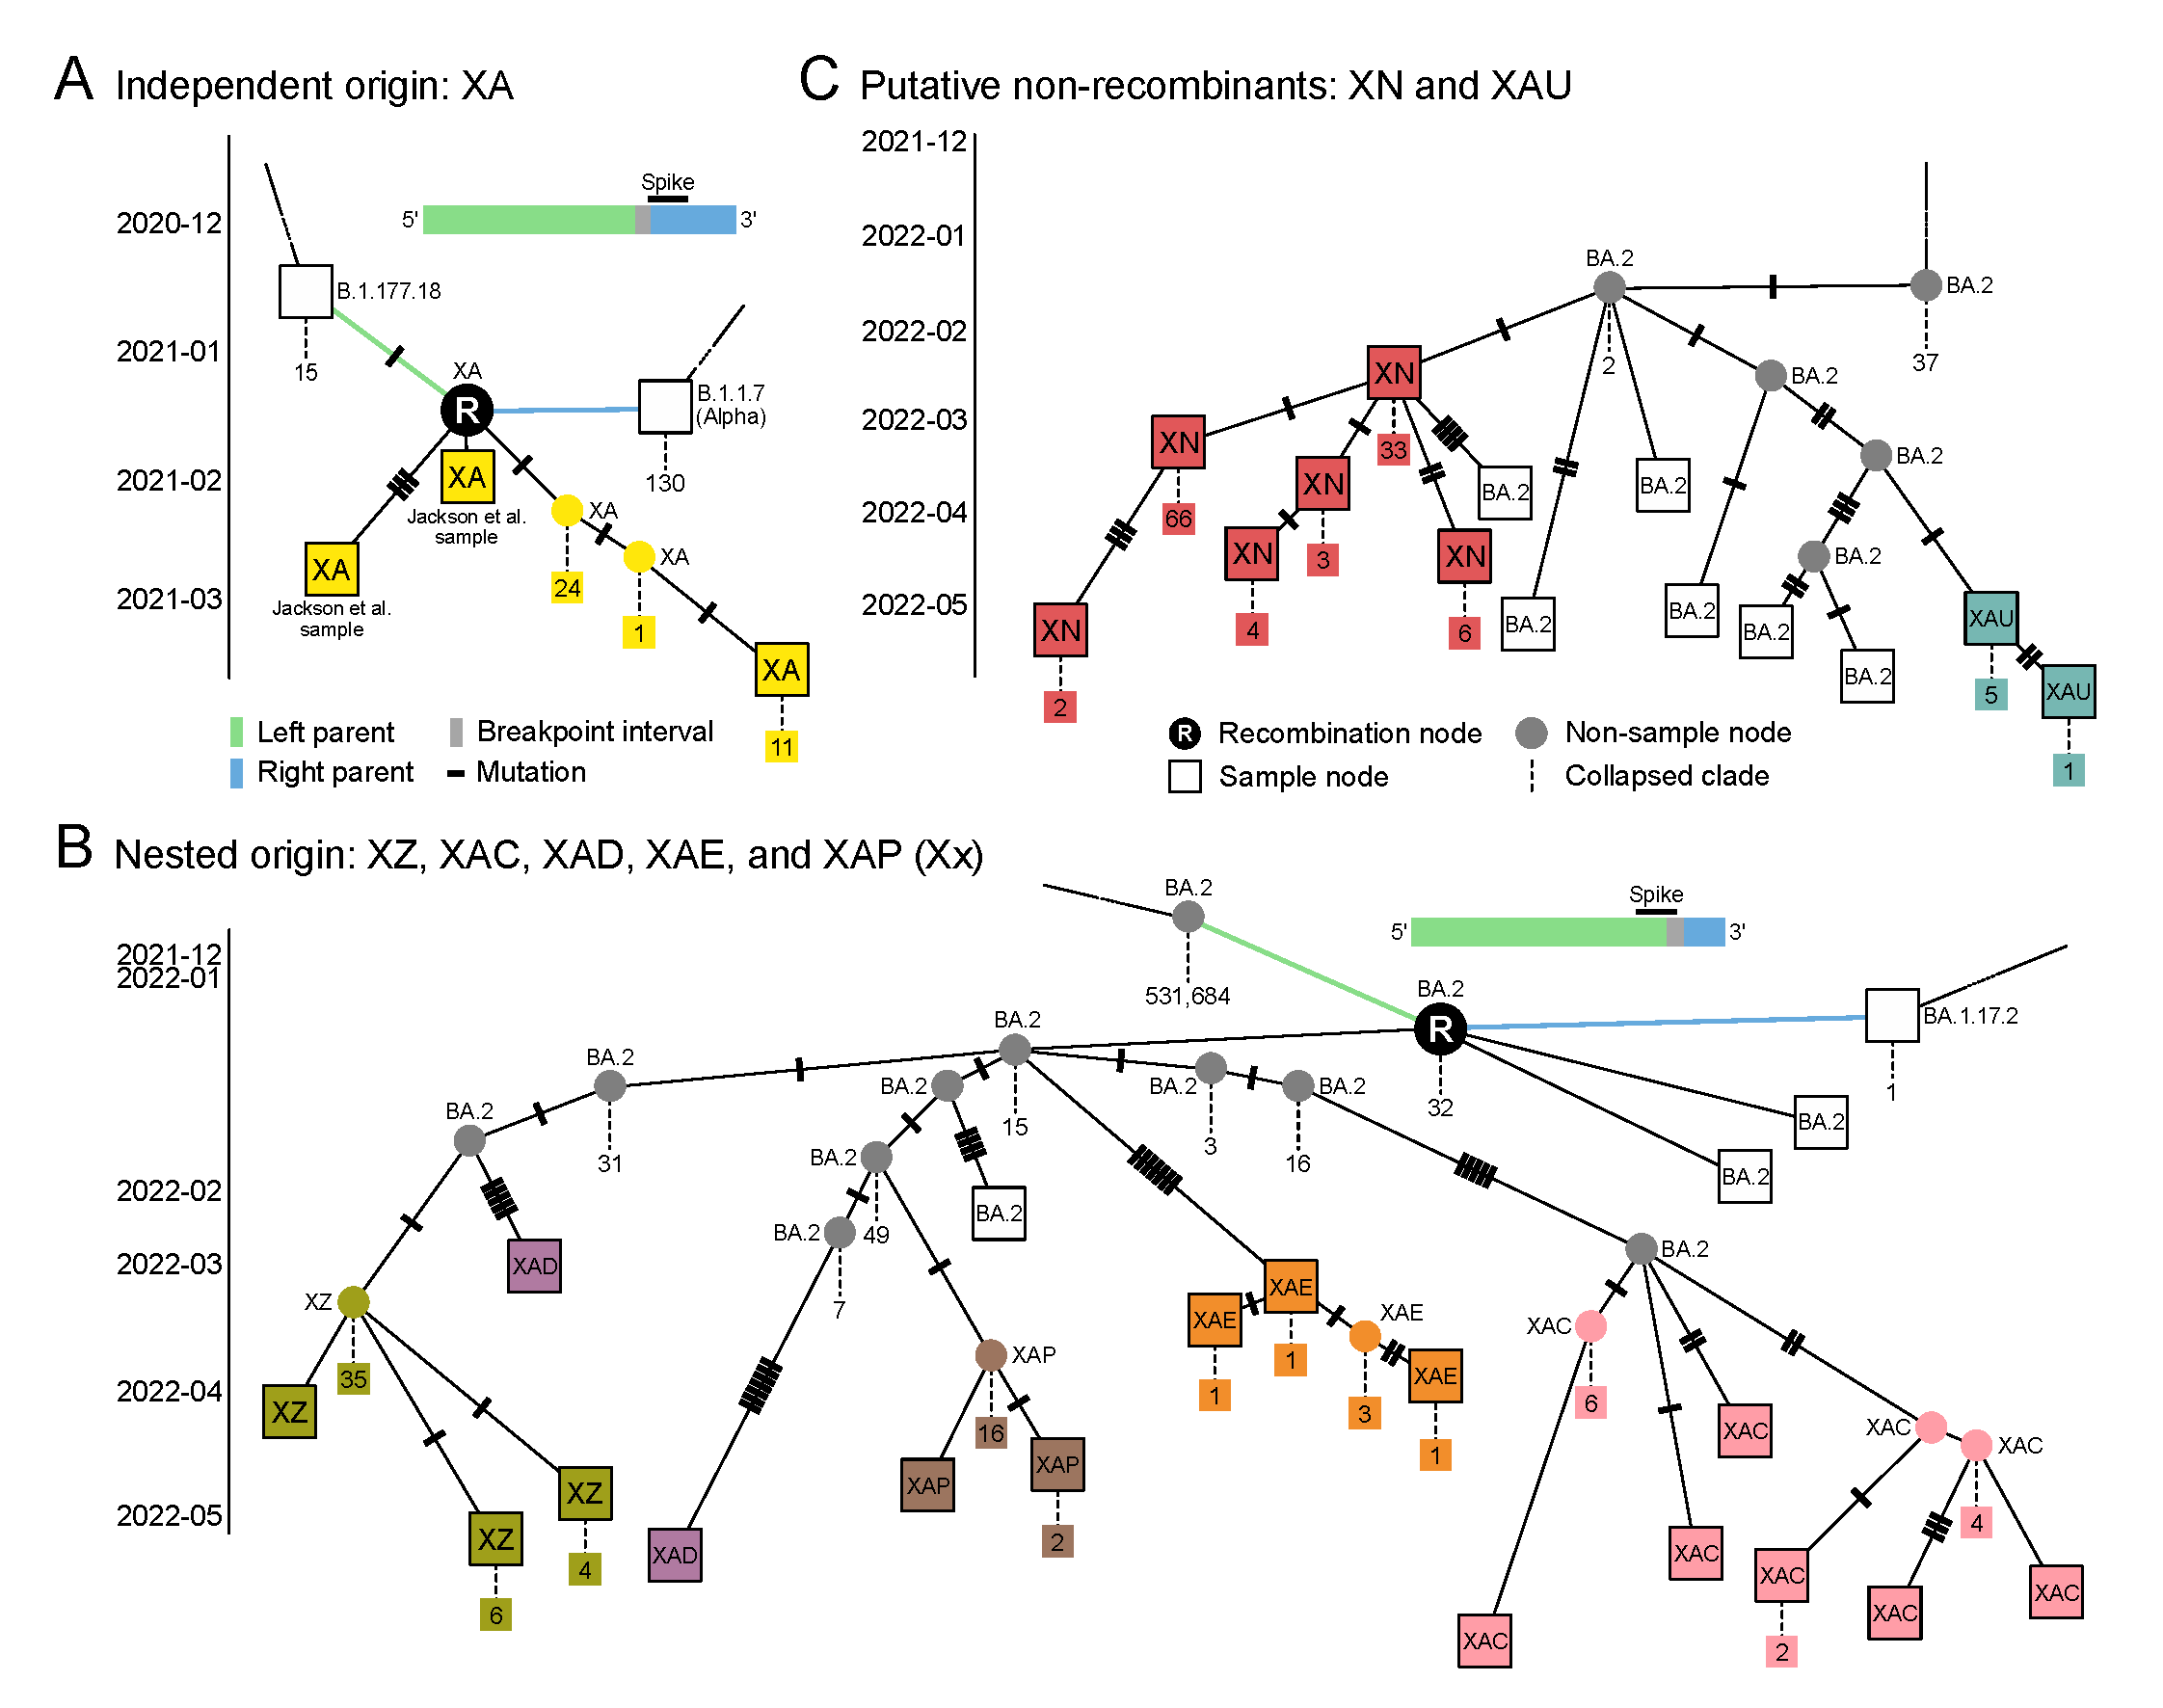
\includegraphics[width=\linewidth]{pango_x_subgraphs}
\caption{
Illustrative subgraphs in the ARG.
(A) Subgraph around the recombination node associated with the XA.
Two "Group A" recombinant samples reported by Jackson et al. \cite{Jackson2021}) are shown.
(B) Subgraph around the recombination node associated with a group of ``nested'' Pango X lineages; and
(C) Subgraph around the MRCA of the closely related non-recombinants XN and XAU.
The nodes assigned to a Pango X lineage are colored by that lineage.
The numbers inside the colored boxes indicate
the number of samples assigned to the Pango X lineage indicated by the same color.
The numbers below the vertical dashed lines indicate
the total number of samples within a collapsed clade.
For each recombination node, a genome schematic shows
the location of its inferred breakpoint interval relative to the Spike gene.
The ancestry above the parents of the recombination nodes or the MRCA is not shown for clarity.
For more detailed visualizations of these subgraphs, see Document S2.
}
\label{fig:subgraphs}
\end{figure}


% This table is generated by the notebook tab_pango_x_events
\begin{table}
\caption{
ARG events associated with Pango X lineages.
Each row corresponds to the oldest node assigned the specified
Pango lineage and the ancestor of all nodes assigned that label
(except XBB, XBB.1 and XM; see STAR methods). [MORE DETAILS]
}
\label{tab:pango_x_lineages}
\begin{footnotesize}
\begin{tabular}{lrrrllrl}
\toprule
\multicolumn{5}{l}{Type I RE event: monophyletic for pango}\\
pango & avt & left & right & left p & right p & samp & nested \\
\midrule
XC & 37 & 26768 & 27390 & \textbf{AY.29} & \textbf{B.1.1.7} & 5 & {} \\
XBR & 22 & 22034 & 22190 & \textbf{BN.3.1} & BQ.1.25 & 1 & {} \\
XA & 16 & 20411 & 21765 & \textbf{B.1.177.18} & \textbf{B.1.1.7} & 39 & {} \\
XS & 11 & 9054 & 10449 & AY.103 & \textbf{BA.1.1} & 17 & {} \\
XL & 8 & 5925 & 8393 & \textbf{BA.1.17.2} & \textbf{BA.2} & 64 & {} \\
XBG & 8 & 22305 & 22917 & \textbf{BA.2.76} & \textbf{BA.5.2} & 25 & {} \\
XQ & 7 & 4322 & 5386 & \textbf{BA.1.1.15} & \textbf{BA.2.9} & 55 & {BA.2:37,
XR:17, XAA:17, XU:1, XAM:21, XAG:6} \\
XBD & 7 & 23020 & 24620 & \textbf{BA.2.75.2} & \textbf{BA.5.2.1} & 30 & {} \\
XM & 6 & 17411 & 21595 & \textbf{BA.1.1} & \textbf{BA.2} & 26 & {BA.2:16,
XAL:3} \\
XBH & 6 & 15452 & 22001 & \textbf{BA.2.1} & BA.2.75.2 & 6 & {} \\
XBB & 6 & 22332 & 22577 & \textbf{BA.2.10} & BM.1.1.1 & 6452 & {BA.2:1} \\
XY & 5 & 11538 & 12880 & \textbf{BA.1.1} & \textbf{BA.2} & 23 & {} \\
XF & 5 & 5387 & 6402 & \textbf{AY.4} & \textbf{BA.1} & 16 & {} \\
XBF & 5 & 5184 & 9866 & \textbf{BA.5.2.1} & CJ.1 & 185 & {} \\
XW & 4 & 2833 & 4321 & \textbf{BA.1.1.15} & \textbf{BA.2} & 32 & {} \\
XG & 4 & 5925 & 6513 & \textbf{BA.1.17} & \textbf{BA.2} & 3 & {} \\
\midrule
\multicolumn{5}{l}{Type II RE event}\\
alias & avt & left & right & left p & right p & desc & by pango \\
\midrule
Xx & 6 & 24504 & 26060 & \textbf{BA.2} & \textbf{BA.1.17.2} & 253 & {BA.2:156,
XZ:48, XAP:20, XAC:18, XAE:9, XAD:2} \\
XE/XH & 6 & 10448 & 11283 & \textbf{BA.1.17.2} & \textbf{BA.2} & 1156 &
{XE:1116, BA.2:37, XH:2, XAF:1} \\
XBM & 6 & 22305 & 22917 & \textbf{BA.2.76} & \textbf{BF.3} & 12 & {XBM:10,
BF.3:2} \\
XAF & 5 & 10199 & 10447 & \textbf{BA.1.1} & \textbf{BA.2} & 36 & {BA.2:35,
XAF:1} \\
XJ & 5 & 13196 & 17410 & \textbf{BA.1.17.2} & \textbf{BA.2} & 85 & {XJ:68,
BA.2:17} \\
\bottomrule
\multicolumn{5}{l}{Events closely derived from RE}\\
pango & alias & path len & time & mutations & samples \\
\midrule
XR & XQ & 3 & 11 & 4 & 17 \\
XU & XQ & 6 & 103 & 13 & 1 \\
XAM & XQ & 6 & 40 & 3 & 21 \\
XAA & XQ & 6 & 33 & 3 & 17 \\
XAG & XQ & 6 & 53 & 4 & 6 \\
XAP & Xx & 4 & 66 & 1 & 20 \\
XZ & Xx & 4 & 48 & 1 & 48 \\
XAE & Xx & 2 & 47 & 7 & 9 \\
XAF & XAF & 5 & 140 & 8 & 1 \\
XAL & XM & 3 & 65 & 2 & 3 \\
\midrule
\multicolumn{5}{l}{Non recombinant}\\
pango & muts & parent & samples & nested \\
\midrule
XP & 1 & \textbf{BA.1.1} & 45 & {} \\
XN & 1 & \textbf{BA.2} & 120 & {BA.2:1} \\
XBQ & 1 & CJ.1 & 14 & {} \\
XBK & 1 & CJ.1 & 7 & {} \\
XBE & 3 & BA.5.2 & 65 & {} \\
XB & 2 & B.1 & 192 & {} \\
XAZ & 3 & \textbf{BA.5} & 133 & {} \\
XAV & 3 & BA.5.1.24 & 13 & {} \\
XAU & 1 & BA.2 & 8 & {} \\
XAS & 1 & BA.4 & 77 & {} \\
XAN & 5 & \textbf{BA.5.1} & 7 & {} \\
XAJ & 11 & \textbf{BA.2.12} & 18 & {} \\
\bottomrule
\end{tabular}
\end{footnotesize}
\end{table}


\subsection*{Comparison with other recombination detection methods}

%%% TODO: Mention RIPPLES somewhere here? Or just in Discussion?
We compared sc2ts against three state-of-the-art methods that detect inter-lineage recombinants:
RecombinHunt \cite{Alfonsi2024}, CovRecomb \cite{Li2024CovRecomb}, and rebar (https://github.com/phac-nml/rebar).
These methods use the same underlying approach:
they scan candidate recombinant sequences for mutations 
associated with different Pango lineages
without using a phylogeny.

To evaluate the concordance of the methods in
identifying the Pango lineages of recombinant parents and locating recombination breakpoints,
we focus on the Pango X lineages associated with the Type I recombination events (Table~\ref{tab:pango_x_lineages}),
using the data from the Pango designation community (https://github.com/cov-lineages/pango-designation/) as a common comparison.
For RecombinHunt and CovRecomb,
we summarized the detection results for these Pango X lineages (if available)
reported in the original studies \cite{Alfonsi2024,Li2024CovRecomb} (STAR Methods).
For each method, we determined the Pango X lineages
for which the inferred parental lineages and breakpoint intervals
are concordant with those identified by the community (STAR Methods).
We found that the methods performed well overall,
with comparable concordance rates (Table~\ref{tab:method_concordance}),
indicating that sc2ts can characterize recombinants as well as the state-of-the-art methods.

Furthermore, we compared the sensitivity of sc2ts and rebar.
We ran rebar on the ``robust'' recombination events detected by sc2ts (STAR Methods),
and found that 167 (43\%) of them were also detected as recombinants by rebar.
We hypothesize that this disagreement arose from
differences in sensitivity between these methods.
Consistent with this, we found that rebar needs a higher level of divergence between parents
to correctly classify a sequence as recombinant, as shown by
a shorter time to their MRCA (Figure \ref{fig:averted_mutations}B) and
a lower distance between their Pango identity (Figure \ref{fig:averted_mutations}C).


\begin{table}
\caption{
Concordance among methods in characterizing Pango X lineages.
These comparisons focus on the Pango X lineages associated with
the Type 1 recombination events (Table~\ref{tab:pango_x_lineages})
For each method, we calculated the number of Pango X lineages
which have inferred parent Pango lineages and breakpoint intervals
concordant with those proposed by the community.
The denominators indicate the number of Pango X lineages
for which detection results are available from the original studies \cite{Alfonsi2024,Li2024CovRecomb}.
For the Pango X lineages with non-overlapping breakpoint intervals,
the distances between the inferred breakpoint intervals and 
those proposed by the community are shown (median and range).
}
\label{tab:method_concordance}
\begin{tabular}{lccc}
\toprule & \multicolumn{1}{c}{Parent lineages} & \multicolumn{2}{c}{Breakpoint intervals} \\
\cmidrule(lr){2-2} \cmidrule(lr){3-4}
Method & Concordant (\%) & Concordant (\%) & Distance (bases) \\
\midrule
Sc2ts & 14 / 16 (87.5) & 14 / 16 (87.5) & 540.5 (315, 766)\\
RecombinHunt-GISAID & 13 / 15 (86.7) & 10 / 15 (66.7) & 764.0 (4, 1202)\\
RecombinHunt-Nextstrain & 12 / 15 (80.0) & 11 / 15 (73.3) & 1160.0 (559, 2785)\\
CovRecomb & 7 / 8 (87.5) & 4 / 8 (50.0) & 1562.5 (217, 13208)\\
\bottomrule
\end{tabular}
\end{table}


\subsection*{Quantification of evidence for recombination}

%%% SHZ: We may not need this section at all, but I'm keeping it for now.
%%% We should probably have a condensed version of the first paragraph in the Pango X section.
%%% The second and third paragraphs should probably be removed entirely.
Sc2ts provides a method to facilitate the discovery of recombination events,
by comparing how well a sample fits the ARG under a model allowing recombination
versus a model disallowing recombination,
as measured by the number of resulting mutations (Figure~\ref{fig:methodology}).
The more mutations are ``averted'' by allowing recombination,
the stronger the evidence for recombination.
We calculated the number of averted mutations for
all the ``robust'' recombination events (STAR Methods),
which include all the Pango X-associated recombination events
(Table~\ref{tab:pango_x_lineages})
and those studied by Jackson et al. \cite{Jackson2021}
(Table \ref{tab:jackson}).

Our analysis of the number of averted mutations reveals a spectrum of plausibility
across all the ``robust'' recombination events
(Figure~\ref{fig:averted_mutations}A).
Examples of highly plausible recombinants are XA and XBB
(for an extended analysis, see Document~\ref{sec:supplement_indepth_pango_x_lineages}).
The ``copying pattern'' of XA visually confirms
that a high number of recombination-informative sites support the suggested parents 
(Figure~\ref{fig:averted_mutations}D).
XW is an example of a marginally well-supported recombinant.
The initial evidence for proposing XW for designation is four nucleotides associated with the suggested BA.1 parent.
% FIXME What's document S3?
The copying patterns of all the recombination events are shown in Document S3.

[FIXME - discuss BA.5 and the BA.2 event instead.]
Our results suggest that Delta and Omicron BA.2 might have recombinant origins,
but we interpret these results with caution,
as these VOCs are undersampled around the time of their emergence (REF).
Consistent with this, the presence of mutations and conflicting loci matching non-focal parents
observed in the copying patterns of these VOCs (Figure 3D) suggests the existence of
many genetically distinct, unsampled ancestors.
Future work is needed to test whether these VOCs descended from recombination events,
with improved sampling, if possible.


\begin{figure}[h]
\centering
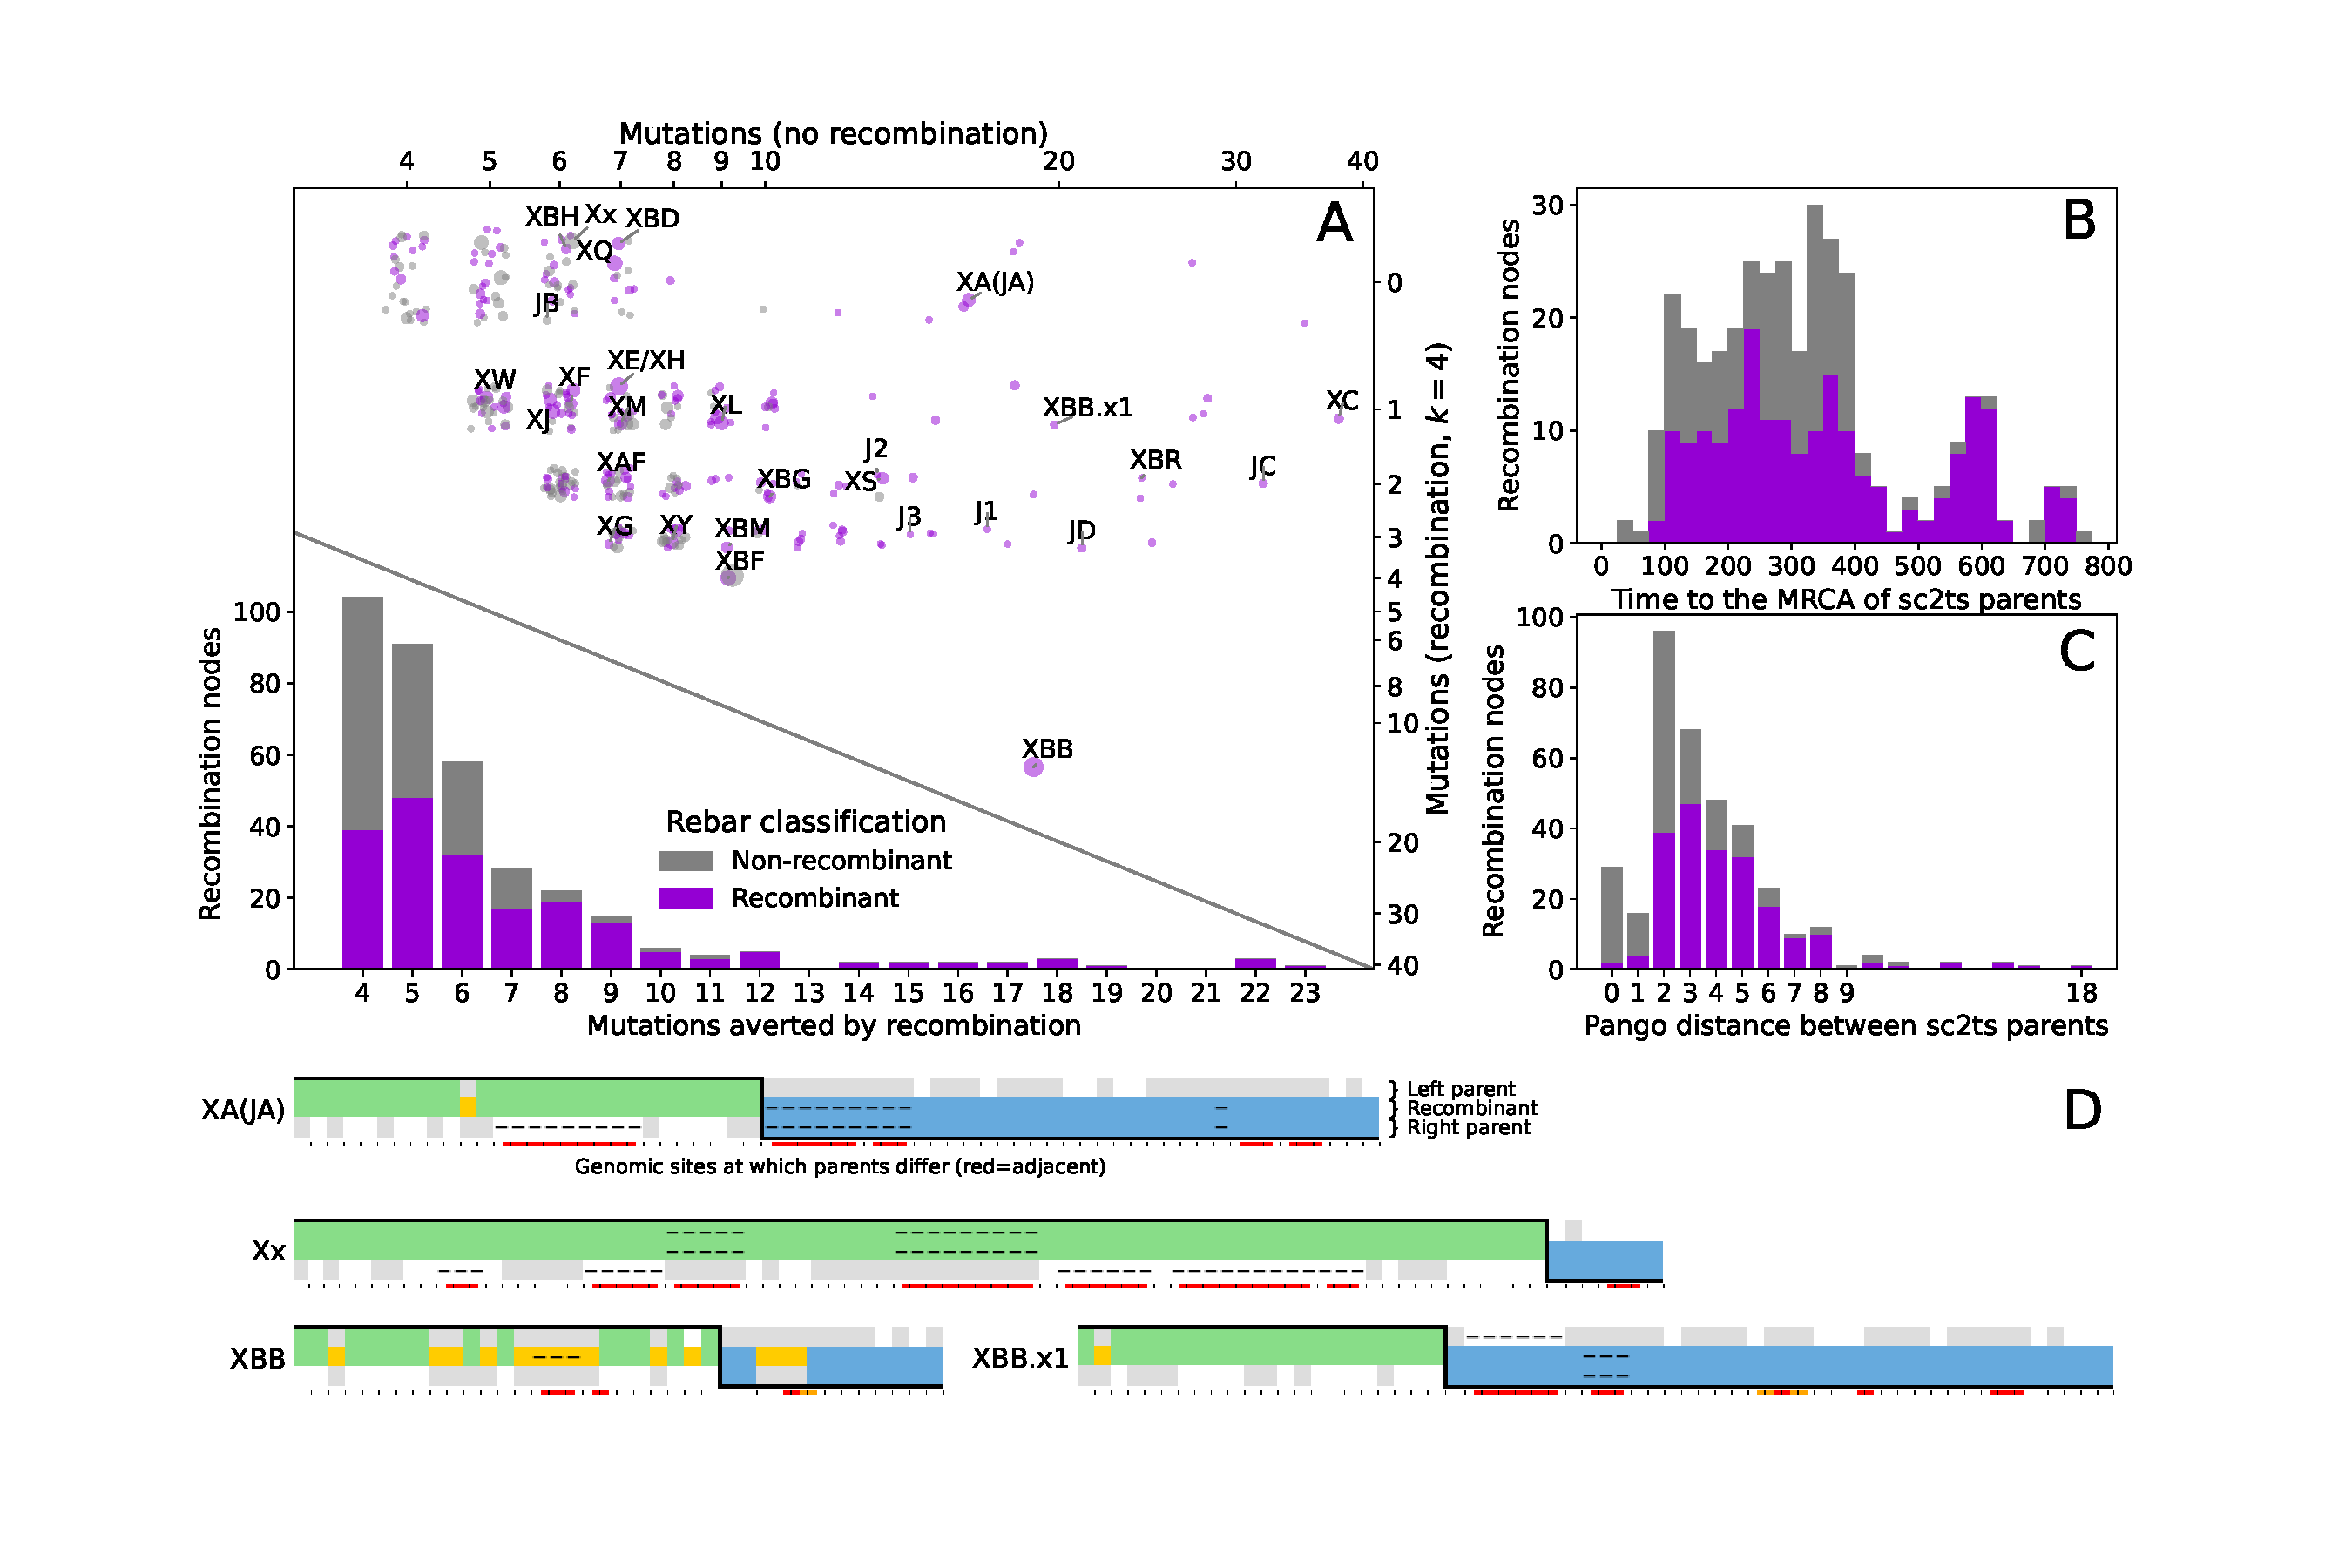
\includegraphics[width=1\linewidth]{recombinant_evidence.pdf}
\caption{
Evidence for recombination in the ARG. All plots show ``robust'' sc2ts recombination nodes,
colored according to their classification by rebar
(recombinant: purple, non-recombinant: gray).
(A) Upper: jittered scatterplot comparing number of mutations
when recombination allowed ($y$: right axis)
versus an alternative copying path disallowing recombination ($x$: top axis);
recombination nodes in Table \ref{tab:pango_x_lineages} are labeled starting with `X' and
those identified by Jackson et al. \cite{Jackson2021} are prefixed with a `J', e.g.
Jackson Group B (JGB) and Jackson Singleton recombinant 1 (JS1).
Point sizes reflect number of descendants.
Lower: recombination nodes classified by number of mutations averted
by allowing recombination (i.e. $x$-$y$).
(B) Distribution of time to the MRCA of the parents of each robust recombination node.
(C) Distribution of the Pango lineage distance between parents.
(D) Copying patterns leading to XA, XBB, XBB.1, and the recombinant origin of XZ+XAC+XAD+XAE+XAP;
each recombination node is a mix of variants matching the left parent (green), the right parent (blue), and de-novo mutations (gold).}
\label{fig:averted_mutations}
\end{figure}


\subsection*{Recombination breakpoint intervals along the genome}

We explored the spatial distribution of the breakpoint locations of
the ``robust'' recombination events along the genome,
and quantified how precisely breakpoints were localized.
For each event, we computed an interval estimate of its breakpoint location,
using its size as a measure of precision (median, 2,207 bases; STAR Methods).

We find an overall preponderance of breakpoint intervals towards the 3’ end of the genome,
particularly at the left boundary of the Spike gene (Figure~\ref{fig:recombinant_intervals}A,B),
consistent with patterns observed in previous studies \cite{Turakhia2022,Li2024CovRecomb}.
While this might result from a higher recombination rate in this region,
it may also be due to the higher levels of polymorphism in the Spike gene,
allowing recombination endpoints to be estimated more precisely.

Furthermore, we find a negative relationship between
breakpoint interval size and the amount of divergence between recombinant parents,
which is measured by time to their MRCA (Figure~\ref{fig:recombinant_intervals}).
When the two parental lineages have diverged for longer periods of time (the rightmost points),
more information becomes available on either side of a breakpoint to pinpoint its location,
resulting in shorter intervals.
For instance, the breakpoint intervals tend to be the smallest for events involving recombination
between the deeply divergent Omicron BA.1 and BA.2 sublineages
(the red points in Figure~\ref{fig:recombinant_intervals}).


\begin{figure}[h]
\centering
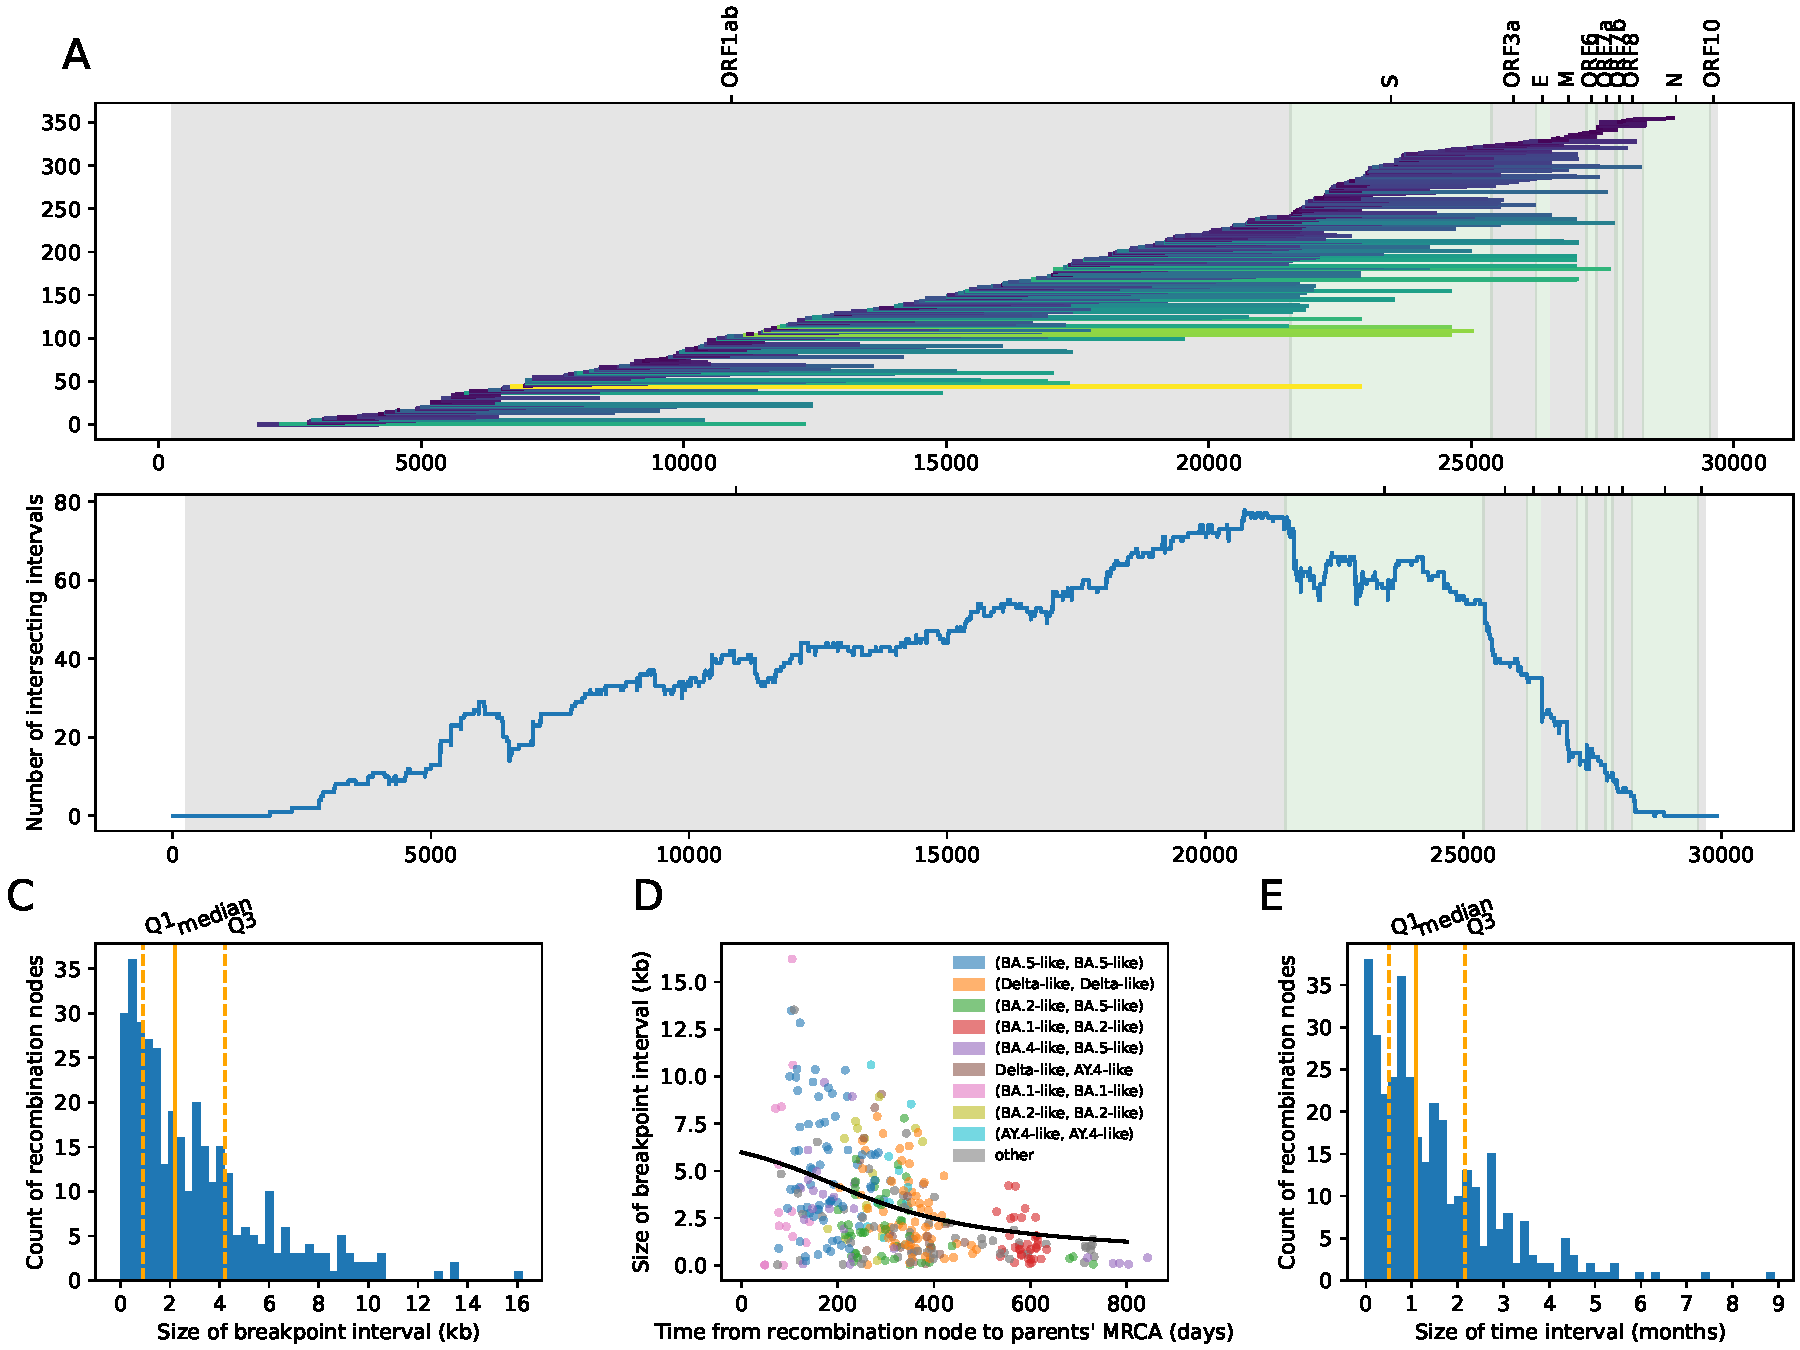
\includegraphics[width=\linewidth]{recombinant_intervals}
\caption{
Recombination intervals.
(A) Distribution of the breakpoint intervals of the 356 robust recombination events along the genome
(annotated with gene labels on top).
Each line represents an interval colored by its size.
(B) Number of overlapping breakpoint intervals.
(C) FIXME Heatmap showing the co-occurrence counts of the parents classified by Scorpio designations.
(D) Relationship between breakpoint interval size and time between the recombination event
and the parental MRCA. The black curve shows the theoretical expected relationship
between these quantities, estimated by minimizing the sum of squared residuals
given a single parameter (the mutation rate) (STAR Methods).}
\label{fig:recombinant_intervals}
\end{figure}


\subsection*{Emergence of recombinants over time}

We examined the frequency of emergence of the recombinants
over the course of the COVID-19 pandemic (Figure \ref{fig:recombinants_over_time}).
We explored two hypotheses for the timing of recombination.
First, we would expect recombination events to occur more often when case counts are high,
which increases the chance of co-infection within an individual, allowing recombination.
Second, we would expect recombination events to be detected more often when lineage diversity is high,
as this increases the chance that two sufficiently distinct viruses co-infected an individual,
increasing our power to detect recombination.

We used the COVID-19 Data Repository at Johns Hopkins University \cite{Dong2020}
to relate the timing of recombination events with global case numbers.
Case numbers ($n$) were binned by week from January, 2020 to March, 2023 and
sub-divided by the proportion in each Scorpio label inferred within the ARG (shading in 
Figure~\ref{fig:recombinants_over_time}).
These lineages correspond loosely to a group of related lineages within a major VOC in the Viridian dataset.
Alongside the case numbers,
the black curve shows the number of recombinants inferred within each week along the ARG,
focusing on the 356 ``robust'' events.
Recombination events were inferred more often during the Delta and Omicron waves, when case counts were high.
Overall, the number of recombinant events rose with the global number of cases
(Figure~\ref{fig:recombinants_over_time}B; 
% JK is this correct?? we had 1.0 + 2.7 \; 10^{-7} x$ which I found confusing
linear regression: $1.0 + 2.7\times 10^{-7} x$, $p = 1.1 \times10^{-7}$).
Recombination events also rose with the diversity of lineages in each week
(Figure \ref{fig:recombinants_over_time}C; linear regression: 
$0.9 + 4.8 x$, $p = 3.4\times10^{-7}$),
measured as the chance that two randomly drawn viruses have different Scorpio designations
($H$, referred to as the ``expected heterozygosity'').

We then asked which single measure best explains the number of recombination events inferred each week,
considering $n$, $H$, $n H$, $n^2$, $n^2 H$.
We included the squared number of cases each week thinking that it might better predict co-infections.
The best single predictor of recombination events involved the product of cases and 
expected heterozygosity ($n H$),
with an adjusted $R^2$ of 23.7\%.
This measure of case diversity ($n H$) explained 49\% more of the variation in recombination events per week
than the next best predictor ($H$, adjusted $R^2$ of 15.9\%).
While consistent with the hypotheses that recombination events occur more often when infection rates are common
and are detected more often when viral diversity is high, we note several sources of uncertainty.
Global case numbers were underreported, particularly during the Delta and Omicron waves \cite{Wang2025}.
Furthermore, there may be substantial uncertainty in the timing of a recombination event,
particularly if these occur in chronically infected individuals (as reported by \cite{Burel2022})
with substantial delays before onward cases are detected.
Finally, the filters that we applied removed all but the most strongly supported recombination events,
although similar conclusions were obtained when all 855 recombinants were considered (STAR Methods).

\begin{figure}[h]
\centering
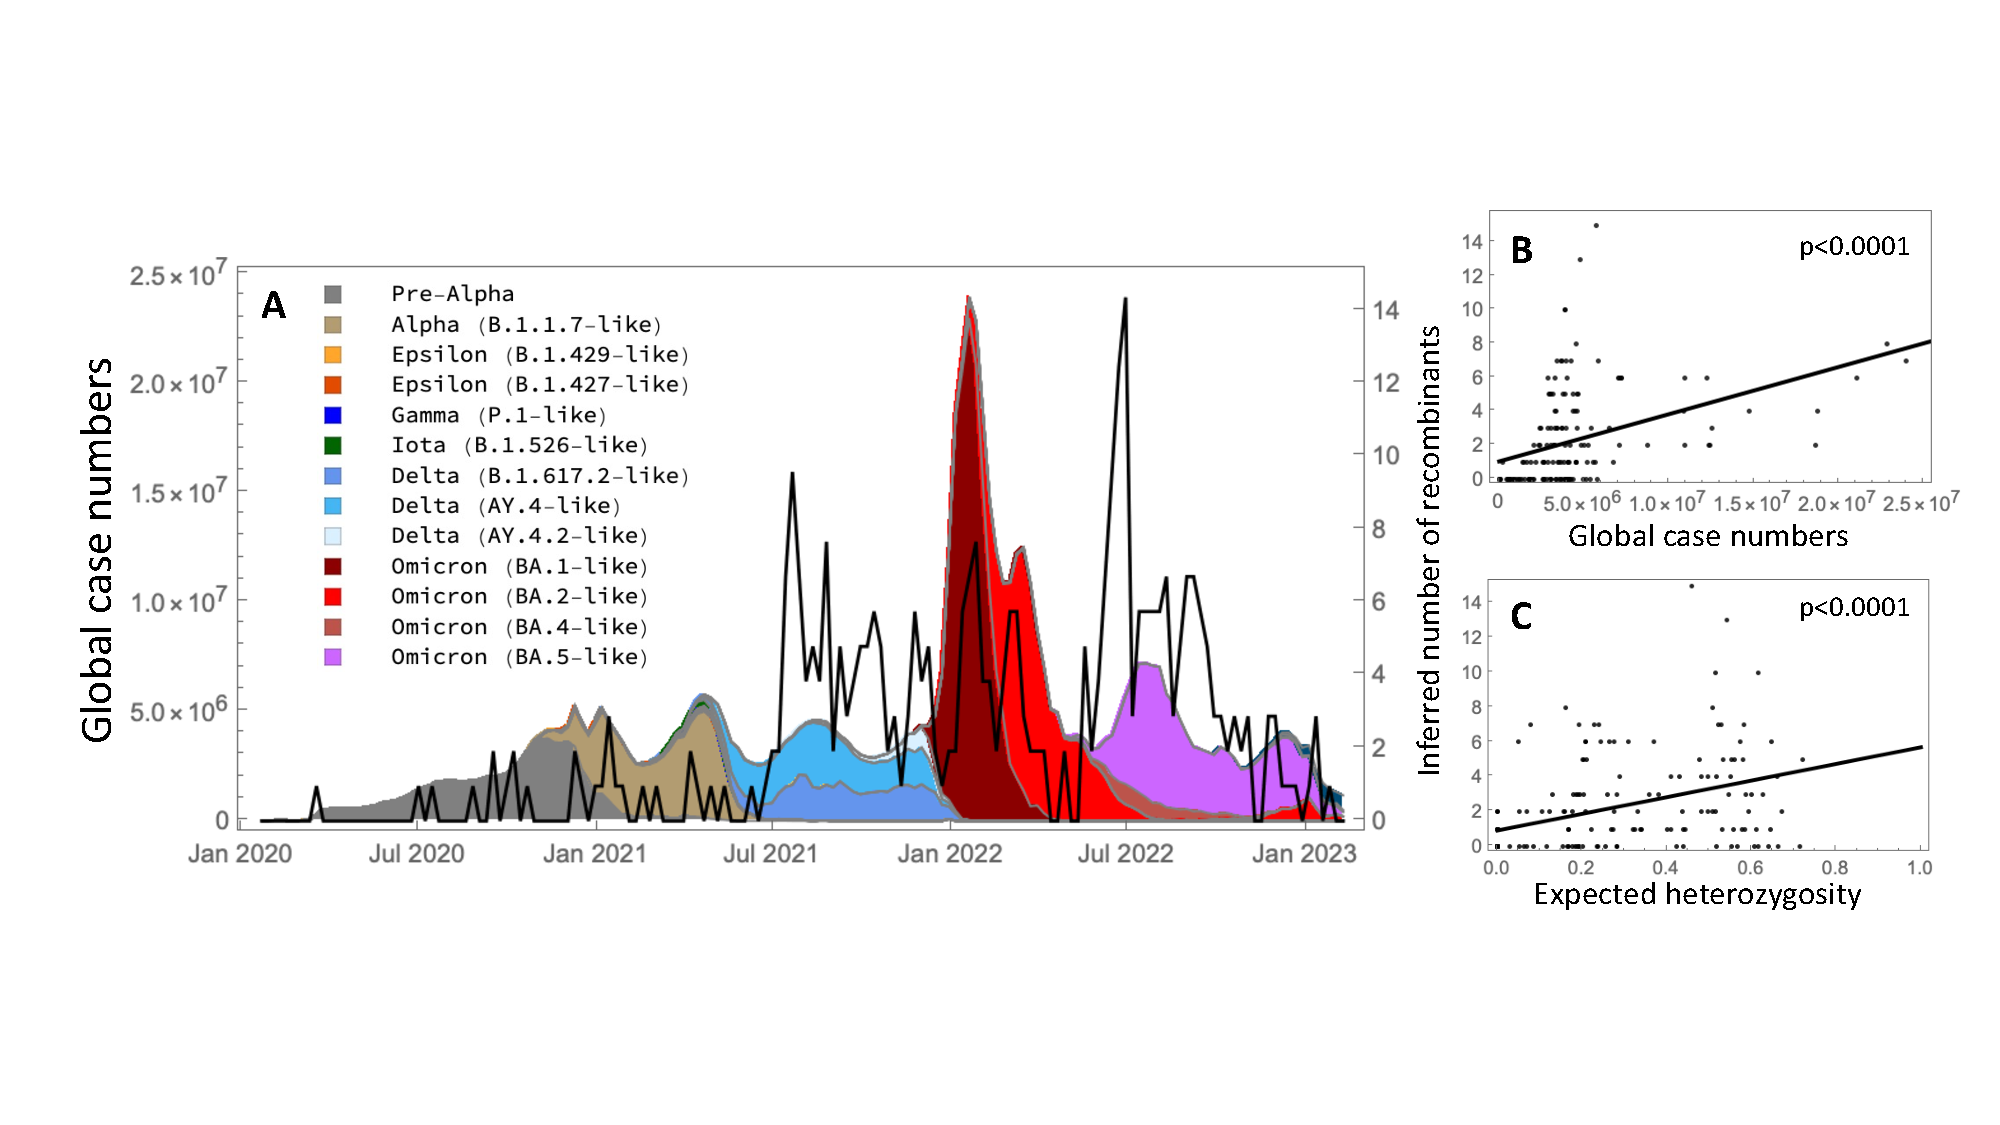
\includegraphics[width=0.85\linewidth]{recombinants_over_time.pdf}
\caption{Recombination events across the pandemic. (A) Timing of the
recombination events (black curve, right y-axis) relative to the global case
numbers (\cite{Dong2020}; left y-axis). Cases are color-coded by their Scorpio
labels, with the key showing those groupings with $\geq 1,000$ samples in the
Viridian dataset. Recombinants more commonly occur (B) in weeks with high case
numbers and (C) in weeks with extensive lineage variation, as estimated by high
expected heterozygosity; solid lines show fits by linear regression, allowing
for non-zero intercepts to account for unknown cases and heterozygosity not
captured by the Scorpio labels.}
\label{fig:recombinants_over_time}
\end{figure}


\subsection*{Efficient inference and analysis of a pandemic-scale ARG}

The COVID-19 pandemic resulted in the collection of viral genome sequence data on an unprecedented scale,
which overwhelmed existing computational approaches,
motivating the rapid development of new methods\cite{Turakhia2021,DeMaio2023,Hinrichs2024}.
Although the computational tools used in phylogenetics and population genetics have historically been largely distinct,
the functionality required largely overlaps.
Sc2ts was built by modifying components of the tskit ARG software ecosystem \cite{Kelleher2019,Ralph2020,Baumdicker2022,Wong2024}
and the VCF Zarr data storage format \cite{Czech2025}
to describe relationships among virus samples, building an ARG over time as data becomes available.
By reusing high-quality and high-performance components of these toolkits,
we could develop the sc2ts inference method itself and
perform all the pandemic-scale analyses in this article with Python code alone and
no compiled languages.

To illustrate the power of these libraries, we provide some examples
in which we compare the Usher and sc2ts intersections in tskit format described earlier.
First, we computed levels of concordance when imputing missing and ambiguous bases in the alignments.
The total aligned dataset for 1,226,587 samples and 27,431 sites shared by the sc2ts and Usher tree sequences
represents 31.34 GB of nucleotide calls.
Of the 80,574,518 missing data calls (Ns) in the alignments,
sc2ts and Usher disagreed in their imputed values for only 56,782 sites (0.07\%).
Additionally, 413,303 calls made use of the IUPAC uncertainty codes.
Of these sc2ts imputed only 77 (0.02\%) incorrectly (i.e., with a base that is not compatible with the ambiguity code).
UShER imputed only 4 calls from this set incorrectly,
reflecting its explicit incorporation of IUPAC uncertainty codes in parsimony calculations.
This computation, performed by co-iterating over the sites in the alignments and the sc2ts and Usher trees,
required 30 lines of Python code and took 2m59s on an intel i7-9700 CPU, with a peak memory usage of about 4.5 GB
(see \cite{Czech2025} for further benchmarks for processing the Viridian data in VCF Zarr format).
Performing this analysis using matUtils would require exporting the full dataset to VCF,
and converting the VCF to FASTA, and then comparing the alignments one-by-one to the source FASTA alignments.
In contrast with matUtils and most phylogenetic software,
which provide a command line interface and suite of predefined operations that typically output text files,
tskit is a Python API (with C and Rust interfaces also supported) which has many advantages \cite{Baumdicker2022}.
As an illustration of the open-ended and efficient nature of the analyses this enables,
we computed the number of polytomies (nodes that have $> 2$ children)
and the maximum number of children per node in the Usher and sc2ts outputs.
In the Usher tree it took 116 ms and 4 lines of code to count polytomies (171,148)
and compute the maximum number of children (5918).
In the sc2ts ARG, it took 385 ms and 6 lines of code to find the maximum number of polytomies (137,001) and
maximum number of children (7708) across all 348 local trees.


\section*{DISCUSSION}

%%% The discussion should explain the significance of the results
%%% and place them into a broader context. Subheadings are permitted.

We present sc2ts, a real-time ARG inference method,
and applied it to build a $\sim$2.48 million-sample pandemic-scale ARG of SARS-CoV-2.
By identifying specific samples as parents,
sc2ts enables more precise interpretation of recombinants than state-of-the-art recombination detection methods,
which find recombinants by matching a given sample to pre-defined population-averaged mutational profiles of Pango lineages.
Sc2ts treats recombination as an integral part of SARS-CoV-2 evolution, in contrast to RIPPLES \cite{Turakhia2022}
which detects recombinants post hoc by searching for unusual branches in a given phylogeny,
inevitably resulting in an incomprehensive representation of SARS-CoV-2 evolution.
Combined with new methods and tools to evaluate evidence for recombination,
sc2ts is a significant technological advance over current methods for the discovery and
analysis of recombinants and efficient inference of SARS-CoV-2 genealogy.

The ARG itself is a useful resource to support future studies of SARS-CoV-2.
Our results show that the ARG captures and unifies important features of SARS-CoV-2 evolution,
which are shown in different studies using different methods, tools, and approaches \cite{Turakhia2022,Bloom2023,Hunt2024}.
The ARG displays remarkable phylogenetic congruence with a state-of-the-art phylogeny built using UShER.
Also, the ARG compactly encodes genetic variation in millions of SARS-CoV-2 genomes,
allowing for convenient and efficient reuse of this valuable dataset
for a variety of evolutionary and genetic analyses beyond those presented here.
% We hope that the ARG will spur on new research areas,
% in which recombination is naturally and fully accounted for,
% and will make an impact comparable to the impact that a recently published human ARG \cite{Wohns2022}
% has made on our understanding of human genetic ancestry and demographic past (e.g., REF).
So far, recent developments in ARG methods have focused almost 
exclusively on applications to human sequencing data. In that space,
the availability of ARGs reconstructed from large datasets has already
had tremendous impact on improving our understanding of human genetic
ancestry and past demography \cite{Wohns2022}. We expect
similar leaps to be enabled through tailoring ARG reconstruction methods
to data from other species and pathogens. Specifically, existing
inference methods can be adapted to use the sc2ts ARG for the 
genealogy-based study of selection \cite{hejase2022deep} or the
geographic spread of the virus through time
\cite{grundler2025geographic}. This is in addition to simpler
analyses, such as calculating mutation spectra or querying the number
or frequency of mutations at a given locus, which the ARG makes 
significantly more efficient, and ultimately more easily reproducible.
Since the ARG is a condensed representation of the genetic information
contained in the sequencing data, it can also be used to understand,
for instance, how the variability in sequencing efforts across time 
and location affects our ability to reconstruct the origin of 
important lineages and detect new recombinants.
Since reconstructing the ARG is computationally expensive, 
and checking and improving various aspects of its quality is laborious, 
we hope that making this resource openly available will save
significant time and 
effort for other researchers and enable immediate focus on analysing 
the information contained within this data. In-depth analysis of the
ARG is also incredibly useful for identifying important directions for
further research, both regarding methods (where current models do not
correctly capture features of the data) and data processing 
(where gaps in sequencing or data artifacts result in clear
reconstruction errors).

We contribute several novel methods and concepts which may find applications beyond sc2ts.
First, we devise a simplified LS model that extends the classic concept of parsimony.
In sc2ts, this model allows for accelerated HMM likelihood calculations,
enabling reconstruction of the pandemic-scale ARG presented here.
Existing HMMs used in statistical genetics may be modified in a similar way for significant speedup.
Second, we propose the concept of mutations averted by recombination,
which leads to an interpretable quantity to weigh the support for 
the hypothesis that a given sample is a recombinant against the hypothesis that it is a non-recombinant,
considering the sampled genetic diversity in an ARG and a specific HMM.
Third, we propose the concept of HMM cost to identify poorly explained samples
which are either too divergent or have a high number of mutations inconsistent with their collection dates.
Here we use HMM cost to reject time traveling samples,
which no existing phylogenetic method detects and handles during inference
(e.g., in the Viridian UShER phylogeny, parent and child nodes do not necessarily follow time order \cite{Hunt2024}),
resulting in a cleaner dataset without samples with wrong collection dates that may affect downstream analyses.
Future work may be estimating dates for the suspected time traveling samples using the ARG provided here
and the sc2ts sample matching engine.

Recombination is an important evolutionary force in viruses \cite{Perez-Losada2015},
but has been understudied in part due to the lack of suitable data models, methods, and tools \cite{Neches2020}.
While the methods and tools developed here are tailored for SARS-CoV-2, they can be extended and adapted for other viruses.
A major advantage of the sc2ts methods and tools is that they are built on top of the mature software libraries of tskit and VCF-Zarr,
which enable pandemic-scale analyses that can be performed on typical laptops.
Both tskit and VCF-Zarr are developed in Python and leverage the popular PyData ecosystem,
making them highly adaptable for a broad range of applications.
Together with the pandemic-scale ARG, we hope that sc2ts will be highly accessible to many researchers,
enabling and accelerating studies of SARS-CoV-2 for years to come.


\subsection*{Limitations of the study}

%%% A "limitations" or "limitations of the study" subsection in the discussion is encouraged
%%% and may be required for some journals and some article formats.

We close by emphasizing several current limitations and potential directions to improve sc2ts.
First, more stringent filters to exclude false positive recombinants during inference
would obviate post-hoc treatment of these recombinants.
Second, indels carry important phylogenetic signals,
for example, as lineage-defining mutations of Alpha and Delta (REF).
We currently treat multi-base deletions as missing data or multiple independent deletions,
but they are in reality single events.
More sophisticated treatments of multi-base indels in the HMM could help recover additional signals
(and avoid false signals) of recombination.
Third, the current HMM assumes a simplistic mutation model,
which does not account for documented transition-to-transversion rate bias (REF)
and context-dependent variation in mutation rate (REF).
A more realistic mutation model may help improve inference of local genetic relationships in the ARG.
Fourth, an inherent limitation of detecting recombination from sequence data,
which applies to all methods, is that it is impossible to detect events with few (or no) supporting bases,
as these cannot be distinguished from mutation events.
This limitation makes it particularly challenging to detect events near the termini of linear viral genomes.
Fifth, it is challenging to accurately reconstruct global events
when there are regions with poor sampling and jurisdictions with long delays
before sequences become publicly available (REF).
Revisiting the ARG topology periodically
(e.g., rewinding the ARG a month and repeating with samples that became available later)
and better handling of putative recombinants with suspiciously long branches
(e.g., Delta and Omicron BA.2) might improve the accuracy of the genealogy.
Finally, future developments may account for geography in the HMM,
favouring attachment of samples to geographically close lineages.

\newpage


%%%  The following components should appear after the methods.
%%%  For journals using STAR Methods, these components
%%%  should appear immediately after the discussion
%%%  (after any "limitations" or "conclusions" subsection
%%%  within the discussion).

\section*{RESOURCE AVAILABILITY}

%%%  The resource availability section is required
%%%  for all research articles. This component
%%%  has 3 subsections: "lead contact," "materials
%%%  availability," and "data and code availability."
%%%  All 3 subsections must be included, even if no
%%%  unique materials were generated in the study.
%%%  Do not edit or change the names of the subheadings.
%%%  No other subheadings or text are allowed in the
%%%  resource availability section.

\subsection*{Lead contact}

%%%  Authors are required to designate a lead contact,
%%%  who will be responsible for communication with
%%%  the journal before and after publication and is
%%%  the arbiter of disputes, including concerns
%%%  related to reagents or resource sharing. Only
%%%  one author can be named the lead contact, and
%%%  only the lead contact’s information may be
%%%  provided in this section.

Requests for further information and resources should be directed to and will be fulfilled by the lead contact, XX (XX@university.edu).

\subsection*{Materials availability}

%%%  This subsection must include a statement describing
%%%  the availability of newly generated materials
%%%  associated with the paper, including any conditions
%%%  for access. If there are no newly generated materials
%%%  associated with the paper, the statement should
%%%  state this, e.g.: This study did not generate new
%%%  materials.

This study did not generate new materials

\subsection*{Data and code availability}
\label{sec:data_and_code_availability}

%%%  All original research papers must include a
%%%  comprehensive and accurate ``data and code
%%%  availability'' statement within the ``resource
%%%  availability'' component of the paper before it
%%%  is accepted for publication. These statements
%%%  are structured and consist of three bulleted
%%%  components. Each component must be present.

[TODO fix the typesetting once all resources are compiled]

\begin{itemize}
\item Snakemake workflow for aligning and converting the Viridian dataset to
VCF Zarr:
\url{https://github.com/jeromekelleher/sc2ts-paper/blob/main/viridian\_dataset/}
\item Complete configuration for running sc2ts base ARG inference:
\url{https://github.com/jeromekelleher/sc2ts-paper/blob/main/inference/viridian\_config.toml}
\item Snakemake workflow for ARG post-processing
\url{https://github.com/jeromekelleher/sc2ts-paper/blob/main/arg_postprocessing/Snakefile}
\end{itemize}

TODO add these to the list above with actual URLs
\begin{itemize}
    \item The ARG and the sequence alignments have been deposited at Zenodo and are publicly available.
    \item All original code has been deposited in GitHub and is publicly available.
    \item Jupyter notebooks to perform the analyses in this paper are available on GitHub.
\end{itemize}


\section*{ACKNOWLEDGMENTS}

%%%  Use this section to acknowledge contributions
%%%  from non-authors and list funding sources,
%%%  including grant numbers.

This work was funded by [FUNDER] via grant [GRANT NO.]. The authors thank all members of the lab for their support.

\section*{AUTHOR CONTRIBUTIONS}

%%%  This component is required for most research papers.
%%%  Mention each individual author with a statement
%%%  outlining the contribution of each author to the work.

Conceptualization, S.C.P. and S.Y.W.;
methodology, A.B., S.C.P., and S.Y.W.;
investigation, M.E., A.N.V., N.A.V., S.C.P., and S.Y.W.;
writing-–original draft, S.C.P. and S.Y.W.;
writing-–review \& editing, S.C.P. and S.Y.W.;
funding acquisition, S.C.P. and S.Y.W.;
resources, M.E.V and C.K.B.;
supervision, A.B., N.L.W., and A.A.D.

\section*{DECLARATION OF INTERESTS}

%%%  This component is required for all articles, even
%%%  if the authors have no competing interests; if
%%%  this is the case, insert "The authors declare no
%%%  competing interests." Please refer to the
%%%  declaration of interests policy:
%%%  https://www.cell.com/declaration-of-interests

S.Y.W. is an employee and shareholder of COMPANY.

\section*{DECLARATION OF GENERATIVE AI AND AI-ASSISTED TECHNOLOGIES}

%%%  If generative AI and AI-assisted technologies
%%%  were used in the writing process, this must
%%%  be disclosed in the paper. This declaration
%%%  does not apply to the use of basic tools for
%%%  checking grammar, spelling, references, etc.
%%%  If you have nothing to disclose, please do not
%%%  include this component.

During the preparation of this work, the author(s) used [NAME OF TOOL OR SERVICE] in order to [REASON].
After using this tool or service, the author(s) reviewed
and edited the content as needed and take(s) full responsibility for the content of the publication.

% \section*{SUPPLEMENTAL INFORMATION INDEX}

% %%%  Supplemental information must be uploaded as
% %%%  separate files. In the main text, please list the
% %%%  files to be included in a brief index. For details,
% %%%  please review the supplemental information guidelines:

% %%%  Journals with STAR Methods:
% %%%  https://www.cell.com/STAR-supplemental-information

% \begin{description}
%   \item Figures S1-SX and their legends in a PDF
%   \item Table S1. A descriptive title for an Excel file that was too large to appear in the PDF
% \end{description}

% \newpage


% \section*{MAIN FIGURE TITLES AND LEGENDS}

% %%%  At final submission, figure files MUST be
% %%%  provided separately as high-resolution image
% %%%  files. All of the panels for a figure should
% %%%  be in the same file. Figures should have
% %%%  clear labels/file names (Figure 1, Figure 2,
% %%%  etc.).

% %%%  Figure titles and legends should be placed
% %%%  at the end of the main text. You do not
% %%%  need to place the figures, nor their titles
% %%%  and legends, within the main text. While
% %%%  typesetting your article, our team will
% %%%  place each figure in the best location
% %%%  based on the final layout and on your
% %%%  figure citations, e.g., (Figures 1A and 1B).

% %%%  Please review the figure guidelines before
% %%%  submitting your final materials:
% %%%  https://www.cell.com/figureguidelines.

% \noindent\includegraphics[width=0.85\linewidth]{Figure1.jpg}

% \subsection*{Figure 1. A brief title that describes the entire figure without citing specific panels}

% The figure legend can be all one paragraph and describe the images (A), graphs (B), and plots (C), etc., together.
% \newline
% (A) Or each panel or group of panels can be described separately, as shown here and below.
% \newline
% (B) Graph of X, Y, and Z.
% \newline
% (C and D) If panels are grouped like this, please explicitly describe each panel, e.g., ``Images showing SEM (C) and TEM (D).''
% \newline
% Please define all scale and error bars, and please review the Cell Press figure guidelines before submission: \href{https://www.cell.com/figureguidelines}{https://www.cell.com/figureguidelines}. Example figure created by Cassie Comeau, Cell Press.

% \newpage

% \section*{MAIN TABLES, INCLUDING TITLES AND LEGENDS}

% %%%  Whenever possible, we encourage you to submit
% %%%  your main-text tables as Microsoft Word documents,
% %%%  using Word's table function. This will ensure
% %%%  the best results during conversion. Tables
% %%%  should be numbered Table 1, Table 2, etc. and
% %%%  should not include subpanels (do not use Table 1A,
% %%%  1B, etc.). Give each table a brief descriptive
% %%%  title. Table legends are optional but encouraged.
% %%%  Footnotes (superscript lowercase letters) should
% %%%  be used where necessary to indicate some feature
% %%%  of the data; please do not use bold, italic,
% %%%  colored text, or shading for this purpose. Use
% %%%  separate cells, not line breaks or spaces, for
% %%%  all discrete data elements. Small embedded
% %%%  graphics with color are OK.

% %%%  Like figures, all tables must be cited within
% %%%  the main text, and our typesetting team will
% %%%  place the tables within the typeset paper at
% %%%  the appropriate locations.


% \subsection*{Table 1. A table with clear organization of data}

% \begin{tabular}{|l | l | l | l|}
%  \hline
%  \textbf{Column 1} & \textbf{Column 2} & \textbf{Column 3} & \textbf{Column 4} \\ [1ex]
%  \hline
%  Row A\textsuperscript{a} & 6 & 87,837 & 787 \\ [1ex]
%  \hline
%  Row B & 7 & 78 & 5,415 \\ [1ex]
%  \hline
%  Row C & 545 & 778 & 7507 \\ [1ex]
%  \hline
%  Row D & 545 & 18,744 & 7,560 \\ [1ex]
%  \hline
%  Row E & 88 & 788 & 6,344 \\ [1ex]
%  \hline
% \end{tabular}

% \bigskip

% The table legend (optional) follows the table itself.
% The legend should be used to provide additional info that relates to the table as a whole.

% \textsuperscript{a}Footnotes can be used to provide additional info on specific content within the table,
% such as this footnote to the first row (row A). Do not use footnotes in the table title.

% \textsuperscript{b}More footnotes

\newpage

%%%  REFERENCES: As of 2023, all Cell Press journals
%%%  use Numbered (AMA) style. We recommend placing
%%%  your references in the included "references.bib"
%%%  file.


\bibliography{references}



\bigskip

%%%  In your References, please include only articles
%%%  that are published (online publication and
%%%  preprint servers are OK). Unpublished data,
%%%  submitted and/or accepted manuscripts, abstracts,
%%%  and personal communications should be cited within
%%%  the text only ("unpublished data," "data not
%%%  shown," "Alice Smith, personal communication")
%%%  and not included in the references list. Personal
%%%  communication should be documented by a letter
%%%  of permission. Whenever possible, please make
%%%  sure your .bib file has the complete author lists
%%%  for each item (at minimum, the first 11 authors
%%%  listed).

\newpage






%%% All Cell Press \textbf{life and medical science} journals, and the multidisciplinary journal \textbf{iScience},
%%% use the \textbf{\href{https://www.cell.com/star-authors-guide}{STAR Methods}} format for reporting materials and methods.

%%% If you are publishing in a STAR Methods journal, please refer to the appropriate guide for authors:
%%% Cell authors should download the guide https://www.cell.com/pb-assets/journals/research/cell/methods/Methods_Guide_Cell-1678470557763.pdf.


\section*{STAR METHODS}

%%%  The STAR Methods should appear in your main
%%%  manuscript file after the figure legends, main
%%%  table(s) and table legend(s).

% \subsection*{Key resources table}

% \textit{To create the KRT, please use the \href{https://star-methods.com}{KRT webform} or the \href{http://www.cell.com/pb-assets/journals/research/cell/methods/table-template1.docx}{Word template} and upload this file separately.}

\subsection*{Method details}

%%%  Please provide precise details of all the
%%%  procedures in the paper (behavioral task,
%%%  generation of reagents, biological assays,
%%%  modeling, etc.) such that it is clear how,
%%%  when, where, and why procedures were
%%%  performed. We encourage authors to provide
%%%  information related to the experimental
%%%  design as suggested by NIH and ARRIVE
%%%  guidelines (e.g., information about
%%%  replicates, randomization, blinding, sample
%%%  size estimation, and the criteria for
%%%  inclusion and exclusion of any data or
%%%  subjects).

\subsubsection*{Ancestral Recombination Graphs}

%%% This paragraph needs to be rewritten.
Originally introduced (Griffiths, 1991; Griffiths and Marjoram, 1997)
to define an alternative formulation of the coalescent with recombination (Hudson, 1983),
the term ``Ancestral Recombination Graph'' has come to be used
more generally to describe not just realizations of the model,
but any recombinant genetic ancestry (Minichiello and Durbin, 2006).
While there is some subtlety in the details \cite{Wong2024},
we can think of an ARG as being any graph
that encodes the reticulate genetic genealogy of a sample of sequences
under the influence of recombination.

The ``succinct tree sequence'' (STS) is an ARG data structure
that is both general (in terms of the types of ancestry that can be described)
and computationally efficient \cite{Wong2024}.
Initially developed to facilitate large-scale coalescent simulations \cite{Kelleher2016},
STS has been extended and applied to
forward-time simulations \cite{Kelleher2018efficient,Haller2019},
calculation of population genetics statistics \cite{Ralph2020} and
ARG inference \cite{Kelleher2019,Wohns2022}.
The STS is based on a simple tabular representation,
which defines a set of nodes, edges, sites and mutations.
A node represents a particular genome, which may be an observed sample or an inferred genetic ancestor.
The genetic inheritance between a pair of nodes along a segment of genome
is defined by the edge ($l$, $r$, $p$, $c$),
which states that child node $c$ inherited its genome from parent node $p$
from left coordinate $l$ to right coordinate $r$.
A site defines a position on the genome and the ancestral state (allele) at that site.
A mutation records the site and node IDs where a mutation occurs and the derived state (allele).

Given the node, edge, site and mutation tables,
we can efficiently construct the local genealogical trees along the genome (arising from recombination)
and perform a range of calculations efficiently
by reasoning about the differences between these local trees \cite{Kelleher2016,Ralph2020}.
These algorithms have led to performance increases of several orders of magnitude over
the state-of-the-art in a range of applications
\cite{Kelleher2016,Kelleher2018efficient,Kelleher2019,Ralph2020,Baumdicker2022}.
The STS encoding is also very concise, allowing, for example,
for millions of complete human genomes to be stored in a few GB of space \cite{Kelleher2019},
and so it is particularly well suited to representing large SARS-CoV-2 genealogies.

The SARS-CoV-2 ARGs inferred using sc2ts can be conveniently and efficiently analyzed
using the mature and feature-rich tskit library \cite{Kelleher2018efficient,Ralph2020}.
Tskit is widely used in population genetics, and has been incorporated into many downstream applications
(e.g., \cite{Haller2019,Speidel2019,TerasakiHart2021,Fan2022,Korfmann2023,Mahmoudi2022,Petr2023,Rasmussen2023,Zhang2023}).


\subsubsection*{Pandemic scale alignment storage}
To provide the efficient access to alignment data required for inference with sc2ts, we
developed a new format based on the VCF Zarr~\cite{Czech2025} specification.
Briefly, Zarr is a storage format for scientific data,
originally developed for the
\textit{Anopheles gambiae}
1000 Genomes Project~\cite{Anopheles2017genetic}, and
is now seeing widespread adoption across the 
sciences~\cite{Abernathey2021cloud,Moore2021ome,Gowan2022using,
Dhapola2022scarf,Virshup2023scverse,Baker2023emobject,Marconato2024spatialdata,Ruan2024image}.
Zarr is essentially a simple mechanism for storing n-dimensional array
data as a regular grid of compressed chunks, which provides 
high levels of data compression, efficient access across multiple
dimensions, and is ideally suited to modern cloud-based
deployments~\cite{Czech2025}. 

We converted the Viridian v05 dataset\cite{Hunt2024}, consisting of 4,484,157 SARS-CoV-2
consensus sequences (125GiB over 48 FASTA files) and 30 metadata fields (1.4
GiB TSV file) to VCF Zarr using a 
reproducible Snakemake\cite{Koster2012snakemake} pipeline.
We aligned each sequence to the Wuhan-Hu-1 reference sequence (MN908947.3) using 
MAFFT v7.475 \cite{Katoh2013},
with the option \texttt{--keeplength} to retain the reference coordinate system.
We then used \texttt{sc2ts import-alignments} and 
\texttt{sc2ts import-metadata} to convert all alignments and metadata to VCF
Zarr format, resulting in a single 401 MiB file 
(around 77X smaller than gzip compressed FASTA\cite{Czech2025}).

A classical tradeoff in bioinformatics is whether to store data 
in sample-major (FASTA) or variant-major (VCF) format, determining
whether the data can be accessed efficiently either by row or column
of the variant matrix. Because VCF Zarr is chunked in two dimensions,
we can now access either sample alignments or the variation
data for a given site across all samples efficiently.
While the VCF Zarr encoding of the MAFFT-aligned Viridian sequences
and metadata can be accessed via native Zarr libraries in several
popular programming languages (see Czech et al.\cite{Czech2025} 
for an overview), the sc2ts Python library provides a convenient interface. 
The \texttt{sc2ts.Dataset}
class provides efficient access to alignments for samples and 
variant data for sites along the genome, as well as methods to export
subsets of the data to FASTA if required.
Document~\ref{sec:supplement_sc2ts_usher_imputation} gives an example
of using this interface, where we retrieve alignment data for millions 
of samples in a few minutes on a standard desktop computer with minimal
memory overhead. See Czech et al.\cite{Czech2025} for more details 
and benchmarks.

Both the pipeline and converted Viridian dataset are available for download;
see Data and code availability for details. 

\subsubsection*{Sample filtering and preprocessing}
The collection date for a sequence is an important piece of information
for sc2ts. We used the Viridian
consensus date (``Date\_tree``), based on information from COG-UK, GISAID, and
ENA/SRA as our source. Samples that have missing or incomplete dates (e.g., 2020-01)
were omitted, as were
the $\sim$40,000 samples which had a collection date of December 31, 2020.
As the sample count for this date is a major outlier for this period of
the pandemic, it seems likely that this 
batch is highly enriched for incorrect collection dates.
Manual checking (by cross-referencing the ENA and COG-UK Mutation Explorer)
confirmed that some of the samples were not collected in 2020.

The bioinformatics community has curated a set of problematic sites
for SARS-CoV-2 that are enriched for systematic sequencing errors or 
high levels of homoplasy~\cite{DeMaio2020issues}. 
Although these sites are recommended to be masked for UShER
inference~\cite{Turakhia2020},
the list has not been updated to take into account the systematic improvements 
made by the Viridian dataset, and we therefore assembled a custom set of sites to mask. 
To do so, we first built a preliminary ARG from the samples collected up to June 30, 2021,
without any site masking.
Then, we identified the top 100 sites in terms of mutation counts in the ARG.
Only 11 of these sites 
(635, 8835, 11074, 11083, 15521, 16887, 21304, 21305, 21575, 21987 and 28253)
were present in the problematic sites file
(\url{https://raw.githubusercontent.com/W-L/ProblematicSites\_SARS-CoV2/master/problematic\_sites\_sarsCov2.vcf}),
and most sites in this list were typical in terms of the numbers of mutations.
We therefore masked our 100 most-mutagenic sites to remove sequencing errors and improve
matching performance in the LS HMM. 

Alignments read from the VCZ Zarr file were first preprocessed to mask any 
non nucleotide characters (A,C,G or T) as missing data. 
Then, we filtered 
any samples that had missing data at more than 500 sites, excluding
the 100 sites identified as problematic (this was 
set to 10,000 sites for the initial period up to 2020-03-01 where sampling
density is low).


\subsubsection*{Li and Stephens haplotype-copying model}

The LS model \cite{LiStephens2003} is an approximation of the coalescent with recombination
that captures many of the key features of the joint processes of mutation and recombination.
It is widely used in a range of applications in population genetics, including ARG 
% Does Threads use LS?
inference \cite{Kelleher2019,Gunnarsson2024}.
The LS model is an HMM that models a focal genome as a sequence of nucleotides (i.e. the observed states),
which are probabilistically emitted as an imperfect mosaic of a set of genomes in a reference panel (i.e., the hidden states).
The process of switching between the genomes in the reference panel is governed by a transition matrix,
and mismatches between a focal genome and a genome of the reference panel (from which it is ``copied'') are permitted as emissions.

In the original formulation of the LS model (see Appendix S1 of \cite{LiStephens2003}),
the probability of switching between the hidden states (i.e., genomes in a reference panel)
when going from one site to the next is dependent on
(1) the rate of recombination between the sites and
(2) the number of genomes in the reference panel ($n$).
Sc2ts uses the same formulation except that $n$ is set to 1.
This special case of the LS model leads to an intuitive interpretation of the ratio
between the probability of switching and the probability of mismatch:
When considering only two copying paths, the path having $k$ mismatches
and the other path having one switch but no mismatch are equally probable.
We call this parameter $k$ the ``recombination penalty''.
% TODO mention that this can be thought of as extended parsimony.
This parameter thus allows us to adjust the relative importance of recombination and mutation
when finding the best explanation for a given sample.
For simplicity, we assume that any single base mutation causing a mismatch is equally probable,
ignoring transition-transversion biases and variation of mutation rate along the genome.
As data sampling was dense for SARS-CoV-2, this assumption was considered tolerable.

We explored using several values of $k$,
by running sc2ts with $k$ set to 3, 4, and 5 on the samples collected in 2020.
We would expect that a good value for $k$ should lead to parsimonious ARGs
that capture plausible recombination events without incurring too many mutations, particularly reversions.
A value of $k$ too low could result in many artifactual recombination events,
whereas a value of $k$ too high could miss many genuine recombination events.
We found that ARGs built with $k$ set to 3 contained many dubious recombination events,
but ARGs built with $k$ set to 5 failed
to include the well supported recombination events documented in a previous study\cite{Jackson2021}.
Hence, we decided to use $k$ set to 4 to infer the final ARG described in this study.

A Viterbi algorithm can be used to find the most likely ``copying path'' of a focal sample
through a reference panel of samples under the LS model.
Specifically, sc2ts uses a Viterbi algorithm modified to operate on STS,
which was originally developed to build genome-wide human genealogies
and is capable of scaling to biobank-scale datasets \cite{Kelleher2019}.
Using this Viterbi algorithm, sc2ts deterministically infers the copying path of a sample
collected on a certain date through the samples collected on earlier dates in a given ARG.

The SARS-CoV-2 sequences were determined from samples collected densely in time.
SARS-CoV-2 phylogenies have low phylogenetic signals due to high sampling frequency
(such that sampling and transmission outpace nucleotide substitution).
Therefore, most samples can be explained by a small number of mutations.
Leveraging this property of the dataset, we developed a likelihood-thresholding strategy
to avoid needing to compute the likelihood of all possible copying paths through an ARG for every single sample.
%%% TODO: This needs to be explained.

[TODO explain Fig S1 and S2]

Furthermore, to avoid performing redundant HMM matching on identical samples, new samples
which were exactly matched to a (sample or non-sample) node in the ARG were not added immediately.
Instead, the copying paths of these samples were recorded,
and the samples were eventually added back to the ARG in a post-processing step.


\subsubsection*{Tree inference from daily sample clusters}
With tens of thousands of samples being added to the ARG per day,
there are often clusters of hundreds of sequences with the same
LS Viterbi solution. That is, large clusters of samples attach
to the same node (or more generally, the same recombinant path)
in the ARG. While some of these samples will require no extra mutations
(as they are identical to the attachment node),
in general there will be complex patterns of shared mutations among the samples
reflecting their evolutionary relationships.
We use a standard neighbor-joining algorithm\cite{Saitou1987}
to infer these within-cluster evolutionary relationships.
We first compute the Hamming distance between
all pairs of samples using scipy~\cite{Virtanen2020scipy},
and then use biotite\cite{Kunzmann2018biotite,Kunzmann2023biotite}
to compute the neighbor-joining tree.
Then, mutations are mapped back onto this daily sample cluster tree using 
the Fitch-Hartigan parsimony 
algorithm\cite{Fitch1971toward,Hartigan1973minimum} implemented in tskit.
Finally, the resulting tree and mutations are added to the ARG at the attachment node(s)
specified by the shared LS copying path.

\subsubsection*{Parsimony improving heuristics}
Attaching trees built from the clusters of samples that copy from
a particular node is an inherently greedy strategy
and can produce inferences that are clearly unparsimonious.
The final step in adding a daily batch of samples to the ARG
is therefore to perform some local updates that target specific
types of parsimony violations in the just-updated regions of the
ARG. There are currently two parsimony-increasing operations
applied, which we refer to as ``mutation collapsing'' and ``reversion
pushing'' (Figure~\ref{fig:parsimony_ops}).

Given a newly attached node, mutation collapsing inspects its siblings from
previous sample days to check if any of them share (a subset of) the mutations
that
it carries. If so, we increase the overall parsimony of the inference
by creating a new node representing the ancestor that carried
those shared mutations and make that new node the parent of the
siblings carrying those shared mutations.
The patterns of
shared mutations between siblings can be complex, and the current
implementation uses a simple greedy strategy for choosing
the particular mutations to collapse. 
119,844 nodes were 
added to the ARG during primary inference by mutation collapsing.

The reversion push operation inspects a newly added node to see
if any of its mutations are ``immediate reversions''; that is,
are reversions of a mutation that occurred on the new node's
immediate parent. We increase the overall parsimony of the
inference by ``pushing in'' a new node which descends from the
original parent, and carries all its mutations except those
causing the reversions on the newly added node.
52,336 nodes were added to the ARG during primary inference by
reversion pushing.

\subsubsection*{Filtering time travellers}
Time-travelling samples---those in which the recorded collection date differs
substantially from their true collection date---pose significant problems
for sc2ts, and are present at a significant frequency. For example, of the 
43 Scorpio designations present in the Viridian dataset studied, 32 have 
samples present with sampling dates in 2020, including lineages that do not
arise until late 2022. Inserting these time-travellers into the ARG 
at the claimed sampling date causes major issues, and they must therefore be 
filtered out. We use the simple approach of filtering out samples that 
exceed a given ``HMM cost'', i.e., requiring too many mutations or
recombination breakpoints to plausibly represent the steady accumulation
of diversity expected with dense sampling. 
The HMM cost for the Viterbi solution for a sample under the LS model
is $k$ times the number of recombination events plus the number of 
mismatches, where $k$ is the recombination penalty (here, $k=4$).
After some experimentation, we set the recombination penalty to 7, 
disallowing samples that require 8 or more mutations (or, e.g., 1 recombination
and 4 mutations, or 2 recombinations) from immediate inclusion (see next
section) in the ARG. This approach has the benefit of filtering
samples enriched for errors as well as time-travellers.

\subsubsection*{Inserting saltation lineages}
The HMM cost threshold approach outlined in the previous section is 
effective at removing time-travelling samples, but it also filters out 
important evolutionary events such as 
the major ``saltations'' that characterize many VOCs.
These lineages are characterized by a high number of accumulated mutations,
and are hypothesized to emerge from chronic infections
during which the virus is exposed to individual-specific immune selective
% Other refs here for this Sally?
pressures\cite{Otto2021origins,Markov2023}.
To distinguish time travelers from true saltation lineages,
we reevaluate the evidence for each lineage with a high HMM cost as additional samples are added.
If these samples form a sufficiently plausible group over successive days (under criteria
described in the next paragraph) sc2ts adds the group to the ARG as a 
``retrospective sample group'' using same mechanisms as standard
daily sample clusters.

Distinguishing a truly emerging outbreak from different forms of
correlated error is non-trivial, and sc2ts has 5 parameters to fine
tune the behaviour. Firstly, we require at least 10 samples in the
group to ensure there is sufficient support over a time window of 
7 days. Then, we build a local tree of the samples and consider
some tree metrics to evaluate whether the samples within the 
group are closely related. If we have at least 2 mutations 
shared by all samples, there's at most 2 recurrent mutations
within the group and at most 5 mutations unique to each sample, 
the retrospective group is accepted for inclusion.
Although this process is highly hueristic, it successfully 
captured the majority of saltational lineages
such as Alpha (Figure~\ref{fig:subgraph_alpha}), and the 
vast majority of samples were added following the standard
daily sample grouping mechanisms. 
% https://github.com/jeromekelleher/sc2ts-paper/blob/main/arg_postprocessing/logs/sc2ts_v1_2023-02-21_pr_pp_mp_aph_bps_pango_dated_recombinants_report.ipynb
In total, 882,398 daily 
sample groups were added to the ARG, while only 100 were
added via this retrospective grouping mechanism.

The Delta, BA.1, and BA.2 lineages were 
particularly challenging, however, as the initial emergences of 
the saltation lineages were not densely sampled. In this case,
there is little information for the retrospective sampling grouping mechanism
to work with and it is very difficult to distinguish short-term time-travellers
from true outbreak samples. For these cases, we chose specific
high-quality samples with confident dates as ``seeds`` which are 
unconditionally included in the ARG on the specified date.

% We used more seeds, but in practise it doesn't matter and it's just
% complicating the story.
For Delta, we used two seeds: one for B.1.617.1 and 1 samples assigned to
B.1.617.2, [with more details and some references to back up our assertions.
There's some specific info in the Viridian paper on this, I'm sure. 
We should mention long branch splitting here too.]
The resulting subgraph can be see in Figure~\ref{fig:subgraph_delta}.

[TODO revise this paragraph to give some background info, and reference
the Viridian work]
For Omicron BA.1 and BA.2, we used SRR17041376 and SRR17461792, respectively.
We chose SRR17041376 (a sample dated 2021-11-12 from South Africa)
as the BA.1 seed (https://github.com/jeromekelleher/sc2ts-paper/issues/264),
as it could be well explained as as a non-recombinant given the ARG available on its collection date.
For BA.2, we chose SRR17461792 (dated 2021-11-27 from South Africa),
which is the earliest BA.2 sample present in the Viridian v04 dataset.
It is dated later than SRR17041376 (the BA.1 seed),
allowing time for the BA.1 lineage to accumulate enough sampled descendants
and to get established in the ARG.
See Figure~\ref{fig:subgraph_ba1_ba2} for an overview of the resulting 
subgraph.

With the combination of these mechanisms---gradual accumulation 
of diversity through daily sample groups, retrospective group
inclusion and manual seeding---we successfully incorporated all major
lineages in the dataset into the ARG (Figure~\ref{fig:samples_per_day}).

\subsubsection*{Primary ARG inference}
The ``base ARG'' we infer with sc2ts is the starting point for later analyses, 
and this step dominates overall processing time. To summarise, we first 
initialise the ARG using the Wuhan-Hu-1 reference sample (MN908947.3) as the
root node, and then ran the algorithm day-by-day using the parameters 
described in the preceding sections and documented in the configuration file 
(see \nameref{sec:data_and_code_availability}).
As discussed above,
computational resources are dominated by the LS model
(Figures~\ref{fig:samples_per_day},\ref{fig:inference_resources}) with all 
other aspects contributing negligibly.

\subsubsection*{ARG postprocessing}
The first step in ARG postprocessing is to examine putative recombinants to
determine whether a more parsimonious explanation is possible. This is done 
by rematching the inferred recombinant sequence against the ARG pruned back
to include only samples before the date of the recombinant. 

Where the recent ancestry of a recombinant includes a branch containing
large numbers of mutations, it is possible
that a non-recombinant solution could be found by postulating an intermediate
node along that branch, that contains only a subset of those mutations.
In particular, for a given mutation-rich branch, artefactual recombinants may
be found in which one recombinant region matches to
a node like the parent whereas another region matches to a node like the child
of that branch. Such recombinants can be identified by the
presence of recurrent or reversion mutations in the left or right parent branches.
To help remove these recombination events from the ARG, we note the genomic positions
of mutations associated with the recombinant, and identify branches
in their ancestry which have mutations at the same positions. Of these branches,
we chose the one that contains the largest total number of mutations as
a candidate for intermediate node creation. This is done by sorting the
mutations on the branch such that the ones that match the allelic state in the
recombinant are placed above the intermediate node, and the others are left
below the node. We refer to this process as ``long branch splitting'', and it
creates additional nodes which are available for recombinant rematching.

% Data from
% https://github.com/jeromekelleher/sc2ts-paper/blob/main/arg_postprocessing/logs/sc2ts_v1_2023-02-21_rewire-recombinants-report.ipynb
Using recombinant-rematching, 58 recombinants were identified as being more parsimoniously 
explained by matching to existing nodes in the ARG (inserted by 
subsequent parsimony improving heuristics) and 16 by long branch 
splitting. Of these 16 recombinants, two are noteworthy as 
being the origins of the Delta and BA.2 lineages in the ARG.
Both result in substantially fewer mutations (15 fewer for 
Delta, 6 for BA.2) than the previous recombinant HMM solution.
These major saltational lineages highlight the challenges 
of using the LS HMM with highly diverged samples.
We then updated the ARG to remove these 74 artefactual 
recombinants by ``rewiring'' the recombination node to the 
more parsimonious non-recombinant solution. This 
resulted in 16 additional nodes, 182 fewer mutations and reduced
the number of trees along the genome from 348 to 317. The long branches
involved in the origins of Delta and BA.2 originally joined
B.1 to B.1.167 and B.1.1 to BA.1 respectively; they can be seen
in Figure \ref{fig:subgraph_delta} and \ref{fig:subgraph_ba1_ba2}
with inserted intermediate nodes leading to the Delta and BA.2
origination nodes.


% and requires a lot of off-topic explanation.
% It is also noteworthy that the origin of the BA.5
% lineage is identified as non-recombinant when long-branch
% splitting is applied to the daily ARG immediately after 
% its inclusion---for this reason, we have identif

The second postprocessing step performed is to add 1,252,208 samples
detected as exact matches during primary inference back
into the ARG. These are not included in the ARG during 
primary inference to reduce memory usage and improve 
LS HMM performance. 

During primary inference, gap characters (``-'') are masked 
out as missing data, but this excludes both important information
about deletions from the ARG as well as potentially informative 
phylogenetic signal. 
We therefore performed post-hoc parsinony mapping at 163 sites to include 
the effects of deletions and to ensure that all Pango-informative
sites are included in the ARG.
Using deletions with a 
a minimum frequency of 1\% 
(count of sequences divided by 9,149,680 sequences analyzed)
from Table S1 of Li et al.\cite{Li2023indels},
we chose 75 sites to remap.
In addition, we remapped data at 88 sites that were excluded
from primary inference and are defined as Pango lineage 
defining sites by
 Freyja\cite{Karthikeyan2022}
(\url{https://raw.githubusercontent.com/andersen-lab/Freyja/refs/heads/main/freyja/data/lineage\_mutations.json}).
Alignment data for these 163 sites was then mapped to the 
ARG using the Fitch-Hartigan 
algorithm\cite{Fitch1971toward,Hartigan1973minimum} 
implemented in tskit, including the gap character as a state 
along with the 4 nucleotides.
Following this, we iteratively applied the node parsimony 
heuristics in sc2ts until there were no further reductions in 
the numbers of mutations.

% Shifting breakpoints is a minor point, not worth mentioning?
We computed Pango assignments for all 2,747,985 nodes in the ARG by first 
exporting their aligned sequences to a 77GiB FASTA file and 
then running pangolin (version 4.3.1; pangolin-data version 1.29).
The resulting Pango and Scorpio designations were then stored as 
metadata associated with each node in the ARG.

When then estimated non-sample node dates using 
the ``variational-gamma'' algorithm in tsdate\cite{Wohns2022}
version 0.2.3. [TODO Say something above the node ages?]

Finally, we reduced the metadata stored in the ARG to a minimal
set (node sample IDs, along with computed Pango and Scorpio 
designations), encoded to enable efficient columnar access,
and compressed the file using tszip (version 0.2.5). The final 
file requires 32MiB of storage.

This full post-processing pipeline is encoded as a reproducible Snakemake
workflow (see \nameref{sec:data_and_code_availability}).


\subsubsection*{Quality control of recombination events}

[TODO This section needs a full pass. I've merged in a section that was in the
supplement with an extremely terse section on counting supporting loci.
Reference Figure~\ref{fig:recombinant_qc} for the scatter plot and 
labeled quadrants, and Figure~\ref{fig:copying_pattern_examples}
for examples of the corresponding copying patterns. Also reference
any additional examples that we include beyond A-D.]


Sequencing errors in genome assemblies \cite{Turakhia2020},
read misalignments \cite{Hunt2024}, and
multi-nucleotide substitutions (MNS \cite{DeMaio2020issues})
can cause short regions of a sample genome to match more closely
to an alternative genome rather than the true parent.
Such genomic regions can be mistaken for evidence of recombination,
because the LS HMM counts each base separately.
Fortunately, artefactual recombinants caused by this effect can be identified
because they affect multiple adjacent or near-adjacent bases simultaneously.

We devised a quality control (QC) measure based on this observation, and
applied it to each putative recombination event in the ARG.
We examined the genomic positions at which the suggested parents differed in allelic state.
Where such sites clustered closely (3 or fewer bases apart),
we treated the entire cluster of sites as a single \emph{locus}.
For each genomic region identified by the HMM as having a single parent,
we calculated the "net number of supporting loci" by counting the number of loci in the region
that supported the suggested parent minus the number that did not support it.
Finally, with all the recombination events in the ARG having a single breakpoint,
we calculated the net number of supporting loci on the left and right sides of each breakpoint, and
used this to plot the 855 recombination events in Figure~\ref{fig:recombinant_qc}.

This simple QC measure effectively differentiates
artefactual recombination events from those that are well supported.
All the sc2ts-detected recombination events associated with the Pango X lineages (Table~\ref{tab:pango_x_lineages})
occur in the upper right of Figure~\ref{fig:recombinant_qc},
with high numbers of net supporting loci on both the right and left parents.
In contrast, the other regions of the plot, where one or both parents are less well supported,
are dominated by recombination events associated with samples sequenced using a specific protocol (AmpliSeq).
Coupled with closer inspection of copying patterns (see below),
we chose a QC cutoff of four or more net supporting loci on both the left and right side of the breakpoint.
This leads to 354 QC-passing recombination events (Figure~\ref{fig:recombinant_qc}, upper right quadrant),
compared to 501 recombination events
for which there is less support and which may be artefactual (shaded quadrants).

Inspection of the copying patterns for all the recombination events
clearly identified associations between recombination events that failed QC and
known problematic loci in the SARS-CoV-2 genome.
Figure~\ref{fig:copying_pattern_examples} shows illustrative copying patterns
(Q1 to Q4 correspond to the labeled quadrants in Figure~\ref{fig:recombinant_qc}),
in which adjacent sites are underlined in red, and near-adjacent sites (within 3 bases) in orange.
A continuous red+orange underline thus indicates a region treated as a single locus.
Q1 shows a well supported recombination event that passed QC (albeit marginally),
having a net number of supporting loci of 4 on both sides of the breakpoint.
Q2 shows an artefactual recombination event caused by a 9-base Delta lineage-defining deletion.
There are XX (XX\%) of the QC-failing recombination events involving this deletion, and
many cases are affected by a known amplicon dropout caused by this particular deletion \cite{Sanderson2021}
Q3 shows an artefactual recombination event caused by a combination of
this Delta lineage-defining deletion and a known MNS (see below).
Finally, Q4 shows an artifactual recombination event associated with the A507T-T508C-G509A MNS,
which has been identified as a sequencing error due to incomplete read trimming \cite{DeMaio2024}.
There are XX recombination events involving this particular MNS, of which XX\% failed QC.


\subsubsection*{Comparison with UShER}
To facilitate comparison with the sc2ts ARG, we first converted the Viridian 
UShER tree from MAT~\cite{McBroome2021} to tskit format, which has similar
properties but is more general (see the section ``Ancestral Recombination
Graphs``).
We first downloaded the tree in JSON format (tree.all\_viridian.202409.jsonl)
from Figshare
and converted the ARG topology. We then downloaded the protobuf formatted
tree (tree.all\_viridian.202409.pb.gz), and exported the mutations to 
nucleotide format using \texttt{matUtils summary --translate}
(usher version 0.6.3), and translated
these mutations into tskit format. The resulting tszip file 
(usher\_viridian\_v1.0.trees.tsz) contains 5,345,019 nodes, 3,364,841
mutations and requires 29MB of storage space.
We validated that the data was correctly encoded by comparing the 
variant data for the UShER tskit tree sequence against our alignments.
There was an exact match between the non-ambiguous nucleotide calls 
at 27469 sites. At the remaining 39 sites there were a significant 
number of gap characters (deletion calls), suggesting that the mismatches
could be due to differences in the alignments used as input to UShER.
See notebook
\href{https://github.com/jeromekelleher/sc2ts-paper/blob/main/notebooks/validate\_usher\_tree.ipynb}{validate\_usher\_tree.ipynb}
for details.

We then computed intersection ARGs for sc2ts and UShER by 
``simplifying''\cite{Kelleher2018efficient,Wong2024} 
both to the 2,475,418 samples and 27,507 sites that are shared.

All conversions were performed as part of the reproducible 
postprocessing pipeline described in [section?]. The full UShER
tree and the intersection files are available for download on Zenodo
in tszip format.

\subsubsection*{Comparison of phylogenetic backbones}

We used Pango lineage designations to select representative samples
for the majority of the 2026 Pango lineages in the ARG.
We first identify an ``origination node" for a focal Pango lineage,
defined as the oldest internal node in the ARG
whose descendants in any tree include more than 50\% of the Pango samples of the focal type,
and where the internal node is itself designated as the focal Pango.
The representative sample is then chosen as the oldest sample descending from the origination node
whose own descendants (if any) are entirely of the focal Pango type.
We ``simplify''\cite{Kelleher2018efficient,Wong2024} 
the ARG to include only the representative samples,
resulting in an intermediate ARG of 1867 samples,
then additionally remove internal samples,
known recombinants (i.e.\ the Pango X lineages) and three ``singleton recombinant
samples''
in which a single Pango lineage appears immediately below a recombination node.
This results in a simplified ARG of 1667 samples, each with a different Pango designation.

We compare topology in the simplified ARG against the UShER tree, built from the Viridian dataset.
To remove time traveling samples from the UShER tree,
we reduce it to 2475419 samples shared with the main sc2ts ARG
and date the internal nodes by running tsdate,
with no rescaling and the root node constrained to the established date of the UShER root (2020-01-16).
To compare against the ARG, we simplify this UShER tree down to the 1667 representative ARG samples.

The simplified ARG contains four single-breakpoint recombination nodes,
corresponding to the origins of Delta, BA.2, BA.5, and a further BA.2 recombinant
which we deem artifactual by our standard criteria
and treat as non-recombinant for the purposes of plotting
(the breakpoint is on the far right at position 27382,
and supported by only 4 distinguishing sites / 3 loci).
To reduce plot density, we consider only those Pango lineages with fewer than 10 samples,
and extract non-recombinant structures from the ARG
by creating a ``base tree'' of 535 Pangos (i.e. excluding all descendants of Delta, BA.2, and BA.5),
a Delta subtree of 160 Pangos,
a BA.2 subtree of 151 sample (excluding BA.5 descendants) and
a BA.5 subtree of 251 samples.
Figure SX shows each of these trees compared against the equivalent dated UShER topology,
with the left and right parents of Delta and BA.2 highlighted in the base tree.
The order of tips in the two trees was chosen to reduce tangling,
as calculated using the NeighborNet algorithm from Dendroscope \cite{Scornavacca2011,Huson2012},
with tanglegrams plotted using the SVG outputting facility built into tskit.
The entire pipeline is saved as a notebook at URL (?).

The majority of resolvable nodes, including most high-level Scorpio groupings,
are shared between the ARG and the UShER tree (magenta nodes).
In the few cases where the trees differ, this is often in terms of degree of resolution of polytomies.
In these cases, sometimes the sc2ts ARG shows greater resolution,
as in the base of the BA.2 subtree, and
sometimes the UShER tree shows greater resolution, as in BA.2.9.


\subsubsection*{Comparison of mutational spectra}

To validate the mutational information contained in the sc2ts ARG,
we compared the all-site mutational spectra of major VOCs in the ARG,
a state-of-the-art UShER phylogeny built using the Viridian dataset\cite{Hunt2024},
and another UShER phylogeny analyzed in a previous study\cite{Bloom2023}.
Mutational spectra are defined as the relative proportions of
each possible type of nucleotide change.

First, we calculated the mutational spectra of Alpha, Delta, Omicron BA.1, BA.2, BA.4, and BA.5
in the sc2ts ARG, considering mutations (ignoring indels) above the sample nodes and internal nodes
which have Scorpio labels associated with the VOCs
(e.g., for Alpha, B.1.1.7-like and B.1.1.7-like+E484K).
These Scorpio labels were assigned to the aligned sequences of the nodes in the ARG using pangolin.
Note that $\sim$98\% of all the mutations in the ARG occur
above the nodes that have a Scorpio label associated with these VOCs
(excluding the nodes with unassigned Scorpio labels).

Next, we calculated the mutational spectra of the same VOCs
using the mutational counts from an UShER phylogeny analyzed in Bloom et al.\cite{Bloom2023},
which was built using a Nextclade pipeline and
has samples collected worldwide up to November, 2022.
To obtain the WHO label corresponding to a Nextclade-defined clade, we used the following mapping:
20I, Alpha; 21I and 21J, Delta; 21K, BA.1; 21L, BA.2; 22A, BA.4; and 22B, BA.5.
The mutation counts were downloaded from https://github.com/jbloomlab/SARS2-mut-spectrum/.

Lastly, we calculated the mutational spectra of the same VOCs
in the Viridian UShER phylogeny\cite{Hunt2024},
which was pruned down to the samples present in the sc2ts ARG.
We used mutations above the sample nodes,
for which Scorpio labels are available
in the Viridian metadata provided by Hunt et al.\cite{Hunt2024}.


\subsubsection*{Comparison with recombination detection methods}

For RecombinHunt, we obtained two sets of detection results of the Pango X lineages
from the supplementary materials of Alfonso et al.\cite{Alfonsi2024}.
One set of results is based on mutational profiles calculated from a global GISAID dataset,
and the other set from a global NextStrain dataset.
The breakpoint intervals identified using RecombinHunt are defined
as the left and right recombination-informative sites.
We adjusted their coordinates by adding one to the right coordinate
so that the intervals are right-exclusive.

For CovRecomb, we summarized the detection results for the Pango X lineages as follows.
First, we obtained the "independent" recombination events
identified by Li et al.\cite{Li2024CovRecomb} (see Table S4 of the study)
which correspond to the Pango X lineages (if available).
When multiple events corresponded to a Pango X lineage,
we took the results of the event which had the highest number of epidemic recombinants.
For other Pango X lineages, we downloaded the full list of putative recombinants
identified in the study
(https://github.com/wuaipinglab/CovRecomb/blob/main/CovRecomb-Global-Version/putative\_recombinants/putative\%20recombinants.csv)
For each of these Pango X lineages,
we took the most commonly observed combination of
the left parent, the right parent, and the breakpoint interval.
The breakpoint intervals are defined as the left and right recombination-informative sites.
We adjusted the breakpoint intervals by adding one to the right coordinate
so that they are right-exclusive.

We ran rebar on the sampled sequences associated with each robust recombination event. 
Rebar identifies a sequence as a recombinant if it contains sets of mutations 
which are pre-determined to be associated with different Pango lineages.

The parents of a Pango X inferred using a method are deemed concordant
if they have Pango lineage assignments
that are at least as specific as those proposed by the community.
The breakpoint interval of a Pango X inferred using a method is deemed concordant
if it overlaps with that proposed by the community by at least one base.
These breakpoint intervals are defined as ranges of possible site positions
where a breakpoint is inferred to occur.
To make these breakpoint intervals right-exclusive,
we adjusted them by subtracting one from the left coordinate and adding two to the right coordinate.


\subsubsection*{Calculation of Pango lineage distance using pangonet}
We define a ``pseudo-phylogenetic'' distance to quantify the divergence between two Pango lineages.
The idea is to count the number of edges separating two given Pango lineages in a ``pseudo-phylogeny''
which relates all the designated Pango lineages.
To construct this pseudo-phylogeny, we used \textit{pangonet},
which mines the information on the Pango lineages in the ``alias\_key.json''
and ``lineage\_notes.txt'' files
from the Pango designation issues (https://github.com/cov-lineages/pango-designation).
If two Pango lineages are siblings in the pseudo-phylogeny,
the distance is defined as the sum of the number of edges from each lineage to their MRCA;
if they are non-siblings (i.e. one Pango is a descendant of the other),
the distance is defined as the number of edges separating them;
if they are identical, the distance is defined as zero.


\subsection*{Quantification and statistical analysis}

%%%  Please describe here all statistical analysis
%%%  and software used. We ask authors to indicate
%%%  in this component where all of the statistical
%%%  details of experiments can be found (e.g., in
%%%  the figure legends, figures, results, etc.),
%%%  including the statistical tests used, exact
%%%  value of n, what n represents (e.g., number
%%%  of animals, number of cells, etc.), definition
%%%  of center, and dispersion and precision
%%%  measures (e.g., mean, median, SD, SEM, confidence
%%%  intervals). Also, please summarize in this
%%%  component how significance was defined, the
%%%  statistical methods used to determine strategies
%%%  for randomization and/or stratification, sample
%%%  size estimation, and inclusion and exclusion
%%%  of any data or subjects, as well as any methods
%%%  used to determine whether the data met
%%%  assumptions of the statistical approach.

\subsubsection*{Estimating interval lengths}
Recombination intervals are imprecise
when the recombining parents are identical in sequence at sites spanning the breakpoint.
Here we estimate the interval lengths expected around a breakpoint,
given a genome-wide mutation rate $\mu$,
total time between two samples ($T$), and
sufficient support to detect the recombination event.
If a breakpoint occurs a fraction $P$ along a genome of length $L$ and
$k$ mutations have occurred to the left of the breakpoint,
then we expect the nearest mutation to occur $P L / (k + 1)$ bases to the left.
If we require $n$ mutations on both sides of the breakpoint,
we can calculate the expected value of the interval to the left by summing across a Poisson-distributed number of mutations,
conditioned on having at least $n$ mutations:

\[I_{left} = \frac{L}{n T \mu} \frac{\Gamma(1+n) - \Gamma(1+n, P T \mu)}{\Gamma(n) - \Gamma(n, P T \mu)}\]

A similar result holds for the right interval ($I_{right}$), but with $P$ replaced with $1–P$.
Summing the two intervals ($I_{left}+I_{right}$) gives the expected interval length.
As detectable recombination events are nearer the center of the chromosome, we use $P=½$ in Figure X.


\subsubsection*{Analyzing global case counts}
To explore the timing of emergence of recombinants,
case count data were downloaded from
the COVID-19 Data Repository by the Center for Systems Science and Engineering (CSSE)
at Johns Hopkins University \cite{Dong2020} and binned by week from January, 2020 to March, 2023.
The proportion of each lineage $i$ in each week ($p_i$) was then inferred
from the Scorpio designation at each node within the ARG for that week.
Genetic variation was measured as the ``expected heterozygosity'' across lineages,
which is the chance that two lineages chosen at random
from that week had different Scorpio designations ($\sum_{i} \sum_{j>i} 2 p_i p_j$).
The linear regression models reported in \textbf{Figure} \ref{fig:recombinants_over_time} allowed for a non-zero intercept,
because there may be unreported cases even without any reported cases.
The slopes were highly significant, and
the p-values were confirmed by randomly permuting the predictor variable 10,000 times.
ANOVAs were conducted to determine which single predictor ($n$, $H$, $n \; H$, $n^2$, $n^2 H$) explained the most variation in recombination events by week.
These statistical tests and graphics were conducted in \textit{Mathematica} 14.2 (Wolfram 2024) and available at GITHUB LINK.

In addition to the analysis of the 356 ``robust'' recombination events with a minimum of four nucleotides supporting each parent,
we analyzed the relationship between the full set of 855 recombinants and case numbers.
These additional recombinants occurred disproportionately during the Delta and first Omicron wave (July, 2021 to February, 2022).
Again, the number of recombinant events rose with the global number of cases
(linear regression: $3.1 + 5.3 \; 10^{-7} x$, $p = 0.0006$)
and with the diversity of lineages in each week
(linear regression: $0.42 + 18.3 x$, $p = 2 \; 10^{-12}$).
The single best predictor of recombination events among the predictors tested ($n$, $H$, $n \; H$, $n^2$, $n^2 H$)
was again the product of cases and diversity ($n \; H$),
with an adjusted $R^2$ of 26.9\%,
although this was now followed closely by expected heterozygosity on its own ($H$),
with an adjusted $R^2$ of 26.5\%.
Thus, similar conclusions are reached with either dataset,
although filtering the recombination events to the 356 with better support revealed a stronger relationship with case numbers.


% \subsection*{Additional resources}

%%%  Please provide links to websites that provide
%%%  further information relevant to the study
%%%  (e.g., protocol download, troubleshooting
%%%  forum, etc.). Clinical trial registry numbers
%%%  and links should also be placed here. Please
%%%  briefly describe the resource and its
%%%  relevance for the paper. Please report this
%%%  information as: ``Description: URL.''

% Cell.com homepage: https://www.cell.com
% \newline Templates for Cell Press authors: https://www.cell.com/article-templates

%%%  ADDITIONAL MANUSCRIPT COMPONENTS:

%%%  Depending on the journal and the article
%%%  type, you may be asked to upload the
%%%  following as separate files: graphical
%%%  abstract, highlights, eTOC blurb (In
%%%  Brief), and/or other article components
%%%  such as a "bigger picture" statement.
%%%  These items are typically not required for
%%%  initial submissions. Please refer to the
%%%  journal's website, your acceptance
%%%  letter, and/or the Final Files
%%%  Requirements checklist to see if any of
%%%  these items are required (at any stage).


\newpage
\setcounter{secnumdepth}{2} % Print out appendix section numbers

\section*{Supplementary Material}
\appendix

\setcounter{table}{0}
\setcounter{figure}{0}
\setcounter{section}{1}
\renewcommand{\thetable}{S\arabic{table}}
\renewcommand{\thefigure}{S\arabic{figure}}
\renewcommand{\thesection}{S\arabic{section}}


\subsection{Analysis of deletions}\label{sec:supplement_dels}

% See https://github.com/jeromekelleher/sc2ts-paper/issues/628
By mapping deletions to the ARG, we identified
important deletion events (Table~\ref{tab:major_dels}),
many of which are associated with the origins of major VOCs,
for example, the deletions in ORF1ab and
S1-NTD (the N-terminal domain of Spike)
associated with the Alpha lineage.
We also identified highly recurrent deletions (Table~\ref{tab:rec_dels}),
for example, two known recurrent deletions in S1-NTD (REF).


Li et al.\cite{Li2023indels} performed a large-scale analysis of indels
using a global GISAID dataset (sampled up to August, 2022).
We examined the major indels reported in Table S1 of Li et al.\cite{Li2023indels}
which have a minimum frequency of 1\% (count of sequences divided by 9,149,680 sequences analyzed).
All of these indels are deletions and have high frequencies in the ARG
(sequence count divided by the total number of samples),
except a 9-base deletion at 11283, a 9-based deletion at 21987, and a 9-base deletion at 686.


\begin{table}
\centering
\caption{Major deletion events in the ARG. These events are inherited by at least 10,000 samples in the ARG. Count is the number of samples inheriting a deletion. The Pango lineage assigned to the node above which an event occurs is shown. Abbreviations: NSP, non-structural protein; ORF, open reading frame; S, Spike; S1-NTD, N-terminal domain in S1 subunit.}
\label{tab:major_dels}
\begin{tabular}{rrcrcrr}
\toprule
Start & Length & Region & Node & Pango lineage & Count & Frequency (\%)\\
\midrule
28271 & 1 & non-coding & 1436808 & B.1 & 1118363 & 45.0561 \\
28248 & 6 & ORF8 & 220186 & B.1.617.2 (Delta) & 1114669 & 44.9073 \\
22029 & 6 & S / S1-NTD & 200039 & B.1.617.2 (Delta) & 1112504 & 44.8200 \\
11288 & 4 & ORF1ab / NSP6 & 1436802 & B.1.1.529 & 871782 & 35.1220 \\
28362 & 9 & N & 1436802 & B.1.1.529 & 871774 & 35.1216 \\
21633 & 9 & S / S1-NTD & 822854 & BA.2 (Omicron) & 532072 & 21.4359 \\
11292 & 5 & ORF1ab / NSP6 & 822854 & BA.2 (Omicron) & 531894 & 21.4287 \\
6513 & 3 & ORF1ab / NSP3 & 851246 & BA.1 (Omicron) & 340757 & 13.7283 \\
11283 & 5 & ORF1ab / NSP6 & 851246 & BA.1 (Omicron) & 339867 & 13.6924 \\
21765 & 6 & S / S1-NTD & 851246 & BA.1 (Omicron) & 339681 & 13.6849 \\
21987 & 9 & S / S1-NTD & 851246 & BA.1 (Omicron) & 339651 & 13.6837 \\
22194 & 3 & S / S1-NTD & 851246 & BA.1 (Omicron) & 312706 & 12.5982 \\
28271 & 1 & non-coding & 86456 & B.1.1.7 (Alpha) & 290446 & 11.7014 \\
11288 & 9 & ORF1ab / NSP6 & 86456 & B.1.1.7 (Alpha) & 290408 & 11.6998 \\
21991 & 3 & S / S1-NTD & 86456 & B.1.1.7 (Alpha) & 288831 & 11.6363 \\
21765 & 6 & S / S1-NTD & 86456 & B.1.1.7 (Alpha) & 290438 & 11.7010 \\
21765 & 6 & S / S1-NTD & 1265302 & BA.4 (Omicron) & 190425 & 7.6718 \\
686 & 9 & ORF1ab / NSP1 & 2698748 & BA.4 (Omicron) & 23330 & 0.9399 \\
\bottomrule
\end{tabular}
\end{table}


\begin{table}
\centering
\caption{Highly recurrent deletions. These are the top 20 deletions in terms of the number of occurrences in the ARG. Abbreviations: NSP, non-structural protein; ORF, open reading frame; S, Spike; S1-NTD, N-terminal domain in S1 subunit.}
\label{tab:rec_dels}
\begin{tabular}{rrcr}
\toprule
Start & Length & Region & Occurrences \\
\midrule
29781 & 1 & non-coding & 12754 \\
29762 & 1 & non-coding & 11383 \\
29779 & 1 & non-coding & 10951 \\
29769 & 1 & non-coding & 10809 \\
29774 & 1 & non-coding & 10735 \\
29700 & 1 & non-coding & 8562 \\
686 & 9 & ORF1ab / NSP1 & 6436 \\
29614 & 1 & ORF10 & 5039 \\
29555 & 1 & non-coding & 4814 \\
29543 & 1 & non-coding & 4804 \\
29541 & 1 & non-coding & 4802 \\
203 & 1 & non-coding & 3604 \\
222 & 1 & non-coding & 3442 \\
21991 & 3 & S / S1-NTD & 2088 \\
28254 & 1 & ORF8 & 1969 \\
28093 & 1 & ORF8 & 900 \\
21765 & 6 & S / S1-NTD & 482 \\
27532 & 1 & ORF7a & 404 \\
335 & 1 & ORF1ab / NSP1 & 370 \\
337 & 1 & ORF1ab / NSP1 & 346 \\
\bottomrule
\end{tabular}
\end{table}


\subsection{Parsimony comparison of sc2ts and UShER}
\label{sec:supplement_sc2ts_usher_parsimony}

We performed an indepth analysis of the sc2ts and UShER ARGs 
(we refer to the UShER tree as an ARG for simplicity here as a single 
tree is also an ARG) in terms of parsimony.
A direct comparison is difficult because of the different aligments 
used as input, the different sets of sites used for inference and 
the fact that we are including deletions for a subset of sites in
the sc2ts ARG. 

When we compare the intersection of the base sc2ts ARG (pre 
site-remapping), sc2ts is very slightly more parsimonious 
% TODO: https://github.com/jeromekelleher/sc2ts-paper/issues/684
with XX mutations over the YYY sites shared between them.
After site remapping, and including all mutations involving 
deletion characters, sc2ts has 143,690 mutations more 
(2,078,370 vs 1,934,680). If we exclude mutations involving 
deletions in sc2ts, this is reduced to 46,371 more (2.3\%)
than UShER.
If we restrict to the 26,192 sites that were not remapped, 
sc2ts has 4,785 (0.26\%) fewer mutations than UShER,
and has around 2.5 times more mutations than UShER on the 
163 sites that were post-hoc remapped.

To provide a more objective measure of the overall parsimony 
of the inferred ARGs with respect to the Viridian alignments,
we remapped all 29903 sites in both ARGs 
using Fitch-Hartigan parsimony. Here the nucleotides
ACGT and ``-'' were treated as distinct characters, with all 
other values regarded as missing data. In this case, the sc2ts 
ARG has 629,864 (5.5\%) fewer mutations (10,840,687 
vs 11,470,551). Some of this difference may be due to the 
post-hoc incorporation of phylogenetic signal from deletions 
by sc2ts, but more work is required to fully understand 
the differences between the two approaches.

See notebook
\href{https://github.com/jeromekelleher/sc2ts-paper/blob/main/notebooks/analysis\_usher\_sc2ts.ipynb}{analysis\_usher\_sc2ts.ipynb}
for details.

\subsection{Imputation comparison of sc2ts and UShER}
\label{sec:supplement_sc2ts_usher_imputation}
Both sc2ts and UShER support missing data in input alignments, and effectively
``hard call'' these values when the samples are integrated into the tree/ARG. 
In doing so, we impute the missing and ambiguous data for these samples.
We evaluate the imputation performance of sc2ts and UShER by comparing their
outputs on the Viridian alignments.

The total aligned dataset for 2,475,418 samples and 27,507 sites 
in the sc2ts and UShER intersection ARGs represents 63.41GiB of nucleotide calls. 
Of the 162,838,461 missing data calls (Ns) in the alignments, sc2ts and UShER
disagreed in their imputed values for only 203,579 (0.125\%). 
Additionally, 956,859 calls made use of the IUPAC uncertainty codes. 
Of these sc2ts imputed 435 (0.05\%) incorrectly (i.e., 
with a base that is not compatible with the
ambiguity code). 
UShER imputed only 7 calls (0.007\%) from this set incorrectly, likely 
due to special handling of ambiguous bases in the parsimony calculations.

This computation is a good example of type of integrated large-scale data analysis 
that can be easily performed using the combination of tskit and VCF Zarr.
The entire analysis is performed in a short Jupyter
notebook~\cite{kluyver2016jupyter}, with the 
core calculation requiring about 30 lines of Python code. Retrieving 
data from the base alignments and ARGs for 2.48 million samples 
at the same time over all 27,507 sites took only 6 minutes, with a peak memory
usage of about 5GiB of RAM on a standard desktop computer.

See notebook
\href{https://github.com/jeromekelleher/sc2ts-paper/blob/main/notebooks/example\_data\_processing.ipynb}{example\_data\_processing.ipynb}
for details.

\subsection{Analysis of Pango lineage ``origination'' events}
\label{sec:supplement_pango_lineages}
To analyze how well the ARG reflects the phylogenetic structure implicit in the
Pango lineage naming system, we considered the Pango assignments generated by
Pangolin on the alignments for each node in the ARG (STAR Methods). If the ARG
perfectly reflected the Pango lineage structure, each lineage would form a
clade descending from a single originating node with that label. We identified
putative origination nodes among those labeled with a given lineage as the node
with the maximum number of descendant samples and the earliest time (if there
is a tie).

Of the 2058 distinct pango lineages in the ARG, 1473 of these (comprising
717798 samples) match perfectly, with unique origination events in the ARG
where all samples assigned a given lineage descend from the first node assigned
that lineage. A further 245 lineages (589197 samples) match perfectly when we
count the descendants of the parent of the first node (accounting for
polytomies in which multiple originating nodes for a given lineage are
siblings). We then have 306 lineages (755840 samples) where the difference in
the number descendants of the first node's parent is $<$ 100. The remaining 35
lineages (420047 samples) are dominated by a few large lineages such as BA.1.1
(147271 samples) and AY.4.2 (54607 samples) which have multiple non-sibling
origins within the ARG.

See notebook
\href{https://github.com/jeromekelleher/sc2ts-paper/blob/main/notebooks/analysis\_pango\_events\_in\_arg.ipynb}
{analysis\_pango\_events\_in\_arg.ipynb}
for details.

\subsection{Additional analyses of the Pango X lineages}
\label{sec:supplement_indepth_pango_x_lineages}

\subsection*{XS}
https://github.com/jeromekelleher/sc2ts-paper/issues/287
In the ARG, the XS samples appear to have originated from two sequential recombination events.
However, the second event is likely an artifact,
as the XS sample associated with this event failed the minimum net number of supporting loci.
In addition, this sample was sequenced using the AmpliSeq V1 kit,
which was also used to sequence eight other samples descending from the same event.
We excluded this likely artifactual event from further analysis and
consider XS to have emerged from a single recombinant origin.

\subsection*{XM}
https://github.com/jeromekelleher/sc2ts-paper/issues/284
Possibly related to deletions.

\subsection*{Multiple breakpoints}
Seven of the Pango X lineages present in the Viridian v04 dataset have more than one breakpoint,
with the supporting evidence documented in the associated Pango designation issues.
Five of these seven X lineages were detected as recombinants by sc2ts.
Three of them (XAY, XBC, XBT) had more than one breakpoint,
but were not added to the ARG due to high HMM cost and
a lack of sample support to be incorporated as retrospective sample groups.
However, the other two (XAC and XAK) had only one breakpoint.

\subsubsection*{XAY}
https://github.com/jeromekelleher/sc2ts-paper/issues/490

\subsubsection*{XBC}
https://github.com/jeromekelleher/sc2ts-paper/issues/486
Sc2ts detected XBC as a three-breakpoint recombinant,
correctly identifying the parental Pango lineages.
The inferred breakpoint intervals mostly overlap with those identified in its designation issue.
XBC was not added to the ARG due to high HMM costs and inadequate sample support
(within a seven-day retrospective time window).

\subsubsection*{XBT}
https://github.com/jeromekelleher/sc2ts-paper/issues/487
Sc2ts detected XBT as a two-breakpoint recombinant,
correctly identifying the parental Pango lineages.
The inferred breakpoint intervals are identical to those documented in its designation issue.
XBT was not added to the ARG due to high HMM cost and low sample support
(only one QC-passing sample in the Viridian v04 dataset).

\subsubsection*{XAC}
https://github.com/jeromekelleher/sc2ts-paper/issues/357
Evidence of the second breakpoint reported in its designation issue relies on
the presence of a large deletion inherited from BA.2*, which is currently treated as missing data by sc2ts.
The XAC samples share a recombination node with the samples of four other 
X lineages
which do not have this deletion (Figure 2C).

\subsubsection*{XAK}
https://github.com/jeromekelleher/sc2ts-paper/issues/484
Our results agree with its designation issue in terms of the parental Pango lineages and breakpoint intervals.
XAK was not added to the ARG due to HMM costs (9 and 10) and insufficient sample support (only two samples).
Interestingly, our results suggest that XAK might be a product of two sequential recombination events.

\subsubsection*{Non-recombinants}
\subsubsection*{XN and XAU}
https://github.com/jeromekelleher/sc2ts-paper/issues/358
https://github.com/jeromekelleher/sc2ts-paper/issues/348
Both of these putative recombinants have been defined on the basis of a RHS from BA.2 and a LHS from BA.1.
In the case of XN, the supposed BA.1 mutations are [C241T, A2832G, C3037T].
In the case of XAU, this set also includes C2470T, so [C241T, C2470T, A2832G, C3037T].
However, both BA.1 and BA.2 are now defined as also having C241T and C3037T.
In addition, a very large number of BA.2 samples also have A2832G, and three BA.2-designated samples also have C2470T.
This means that there is essentially no longer any evidence for a BA.1 parent for XN, and
only one uncertain mutation that suggests a BA.1 parent for XAU.

\subsubsection*{XAS}
https://github.com/jeromekelleher/sc2ts-paper/issues/340
This was proposed as a recombination between BA.5 (LHS) and BA.2 (RHS).
However, we find that this is only 2 mutations different from e.g. ERR9929846 which is a BA.4 sample.
In fact, XAS only differs from the BA.4 root by a single mutation, C27945T,
which was identified in the original designation issue as an important ORF truncation mutation also present in a few BA.2.65 samples.
It is possible that C27945T was acquired by recombination, this is clearly below our threshold for considering something to be a recombinant.

\subsubsection*{XB}
https://github.com/jeromekelleher/sc2ts-paper/issues/332
XB was proposed to have originated from recombination between B.1.634 (left parent) and B.1.631 (right parent).
None of the samples in Viridian v04 belonging to these Pango lineages were integrated into the ARG due to high HMM costs.

\subsubsection*{XP}
https://github.com/jeromekelleher/sc2ts-paper/issues/345

\subsubsection*{XAJ}
https://github.com/jeromekelleher/sc2ts-paper/issues/352

\subsubsection*{XAZ}
https://github.com/jeromekelleher/sc2ts-paper/issues/356
Proposed as a recombinant of BA.2.5 on the left and BA.5 on the right, with 3 supporting sites (C2232T, C3317T, T3358C).
In sc2ts this is very close to being a recombinant of BA.2.5 (ERR9615610) on the left,
as not only are the 3 mutations present in this sample,
but there is another site (C1912T apparently missed in the designation) which supports recombination.
XAZ has C44T which is lacking in all BA.2.5 samples,
giving only three net supporting loci for a putative recombinant.
However, position 44 is often clipped, so this is not strong evidence against a recombinant, and
this is a very finely balanced case.

\subsubsection*{XAN and XAV}
https://github.com/jeromekelleher/sc2ts-paper/issues/353
Below threshold.

\subsubsection*{XBE}
This was proposed as a recombinant between BA.5,5 and BE.4.
We find two net supporting loci for a recombination breakpoint to be around 22599.


\subsection{Analysis of the Jackson et al. recombinants}

Jackson et al.\cite{Jackson2021} conducted detailed analyses of early recombinants
involving B.1.1.7 (Alpha), including the first designated Pango X lineage, XA.
The authors first performed a targeted search for candidate recombinants by
scanning sampled sequences for sequence motifs associated with Alpha,
followed by an analysis to reduce the list of plausible recombinants
displaying signs of onward transmission.
Here we compared the sc2ts detection results of these recombinants
with the detection results reported by Jackson et al.

% Data derived from the notebooks/jackson_recombinants.ipynb notebook
% See https://github.com/jeromekelleher/sc2ts-paper/issues/293
Jackson et al. described four groups of recombinants (named A to D) and
four singleton recombinants.
Of the 16 samples analyzed by Jackson et al, 12 were included in the ARG;
the remaining 4 were excluded because the sequences did not pass the 
QC filtering criteria, or due to a high HMM cost. Groups A-D are summarized 
in Table~\ref{tab:jackson} and show excellent concordance in terms 
of the parental Pango lineages and breakpoint intervals. All four groups
are directly associated with strongly supported recombination events 
in the ARG in terms of the number of averted mutations (A: 16, B: 6, C: 30, D: 18).
The singleton CAMC-CBA018 has 
the parents B.1.177+B.1.1.7 and the breakpoint interval 16,177--20,133 in the ARG, 
and is strongly supported by 14 averted mutations.
The Jackson et al.\ results are almost identical with the same parent lineages, 
and breakpoint interval of interval 11,395–21,993.
The singleton MILK-103C712 has 
the parents B.1.177.16+B.1.1.7 and a breakpoint interval of 24915--27972 
in the ARG, again strongly supported by 11 averted mutations.
The Jackson et al.\ results for this lineage has the same parents,
with the breakpoint interval 26,800–-27,974.
The singleton QEUH-1067DEF has the parents B.1.1.7+B.1.177.9 
and a breakpoint interval of 7,729--10,870 in the ARG, 
supported by 11 averted mutations.
The Jackson et al.\ results for this lineage has the same parents,
with the breakpoint interval 6,953--10,872.


\begin{table}
\centering
\caption{
Comparison of recombination breakpoint
intervals and parent lineages for Groups A-D
reported by Jackson et al.\ with the corresponding
recombination events in the sc2ts ARG.
The second column gives the number of sequences in the group.
See the text for details of the groups and the sequences included.
limited to the samples considered by Jackson et al.
The breakpoint coordinates in Table 1 of Jackson et al.\ have been altered as follows: 
we subtract one to the left coordinates and add one to the right coordinates 
to correspond to the \texttt{tskit} definition of inheritance on either side of a breakpoint,
and add one to the right coordinate to make the intervals right-exclusive.
}
\label{tab:jackson}
\begin{tabular}{lllr@{--}lr@{+}l}
\toprule
Group & Sequences & Method & \multicolumn{2}{c}{Breakpoint interval} & \multicolumn{2}{r}{Parent lineages} \\
\midrule
A (XA)       & 2   & Jackson        &  21,254&21,767 & B.1.177&B.1.1.7 \\
             &     &\texttt{sc2ts} &  20,411&21,765 & B.1.177.18&B.1.1.7 \\
\cmidrule{3-7}
B            & 2   & Jackson        &  6,527&6,956 & B.1.36.28&B.1.1.7  \\
             &     &\texttt{sc2ts} &   6,529&6,954 & B.1.36.28&B.1.1.7  \\
\cmidrule{3-7}
C            & 3   &Jackson         &  24,913&28,653 &  B.1.1.7&B.1.221 \\
             &     &\texttt{sc2ts} &  25,997&27,972 &  B.1.1.7&B.1.221.1 \\
\cmidrule{3-7}
D            & 3   & Jackson        &  21,574&23,065 &  B.1.36.17&B.1.1.7 \\
             &     &\texttt{sc2ts} &  22,445&23,063 &  B.1.36.39&B.1.1.7 \\
\bottomrule
\end{tabular}
\end{table}


\section*{Supplementary Figures}

\begin{figure}
\centering
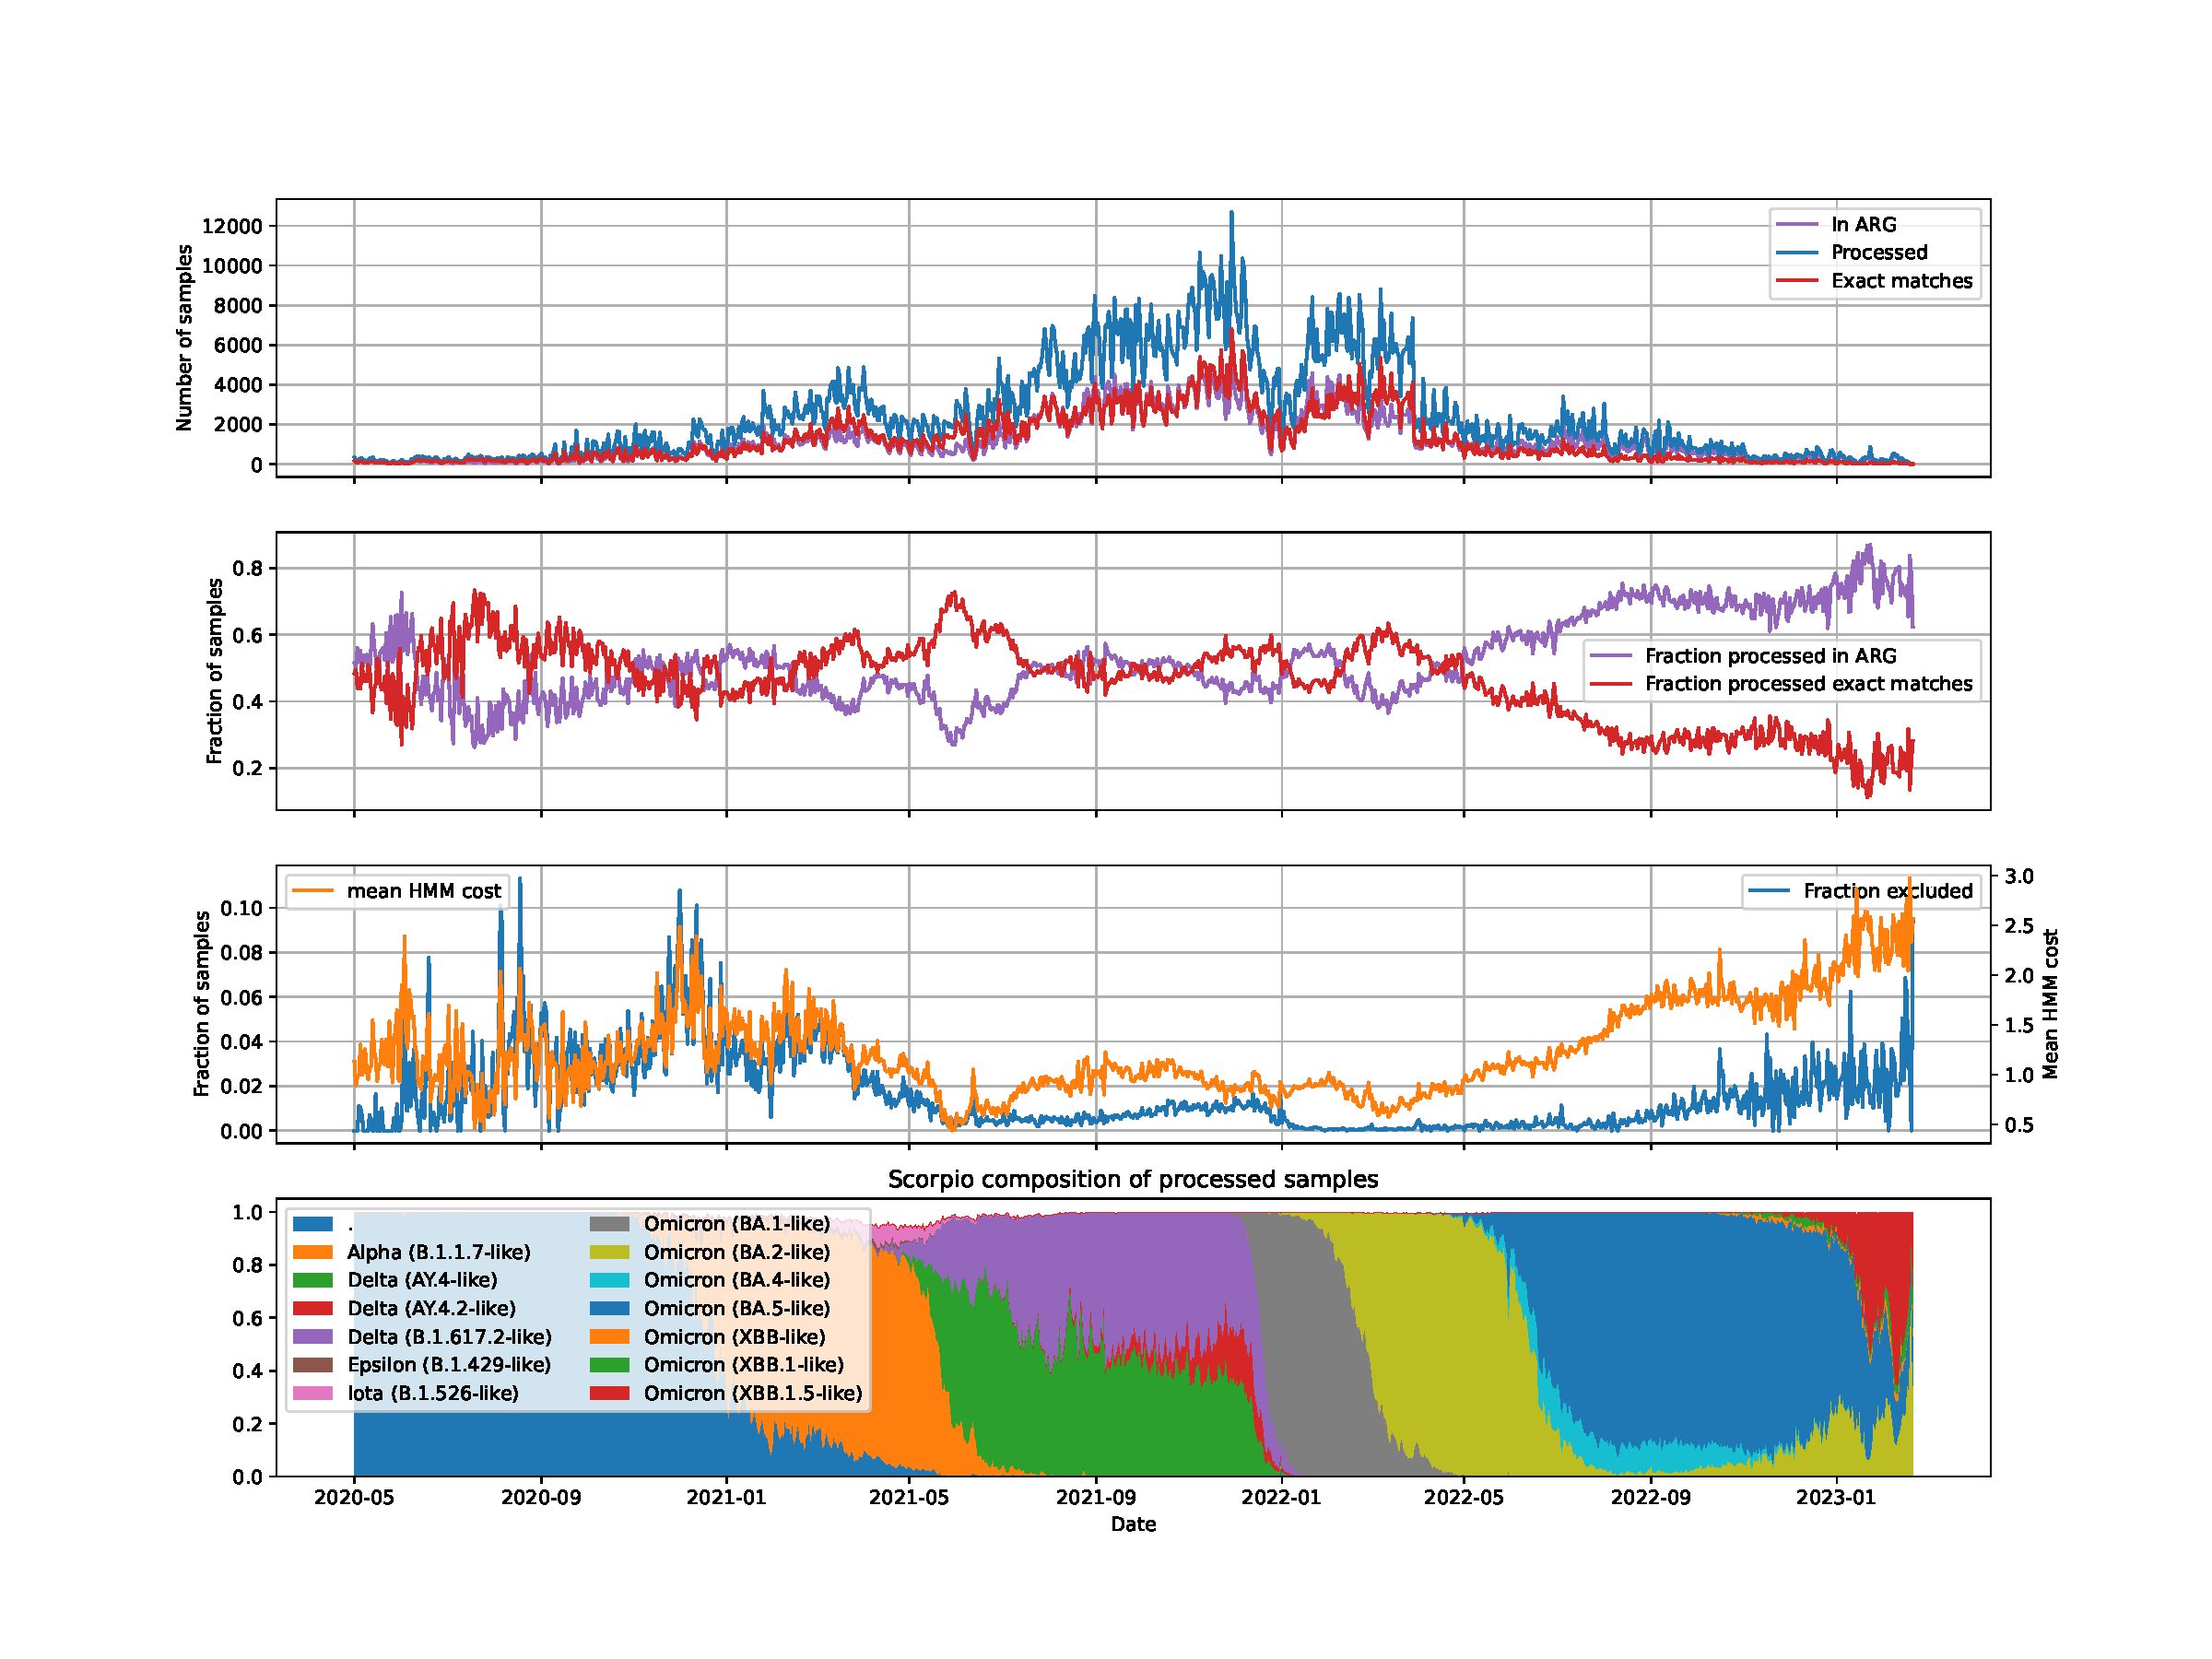
\includegraphics[width=\linewidth]{samples-per-day}
\caption{TODO caption}\label{fig:samples_per_day}
\end{figure}


\begin{figure}
\centering
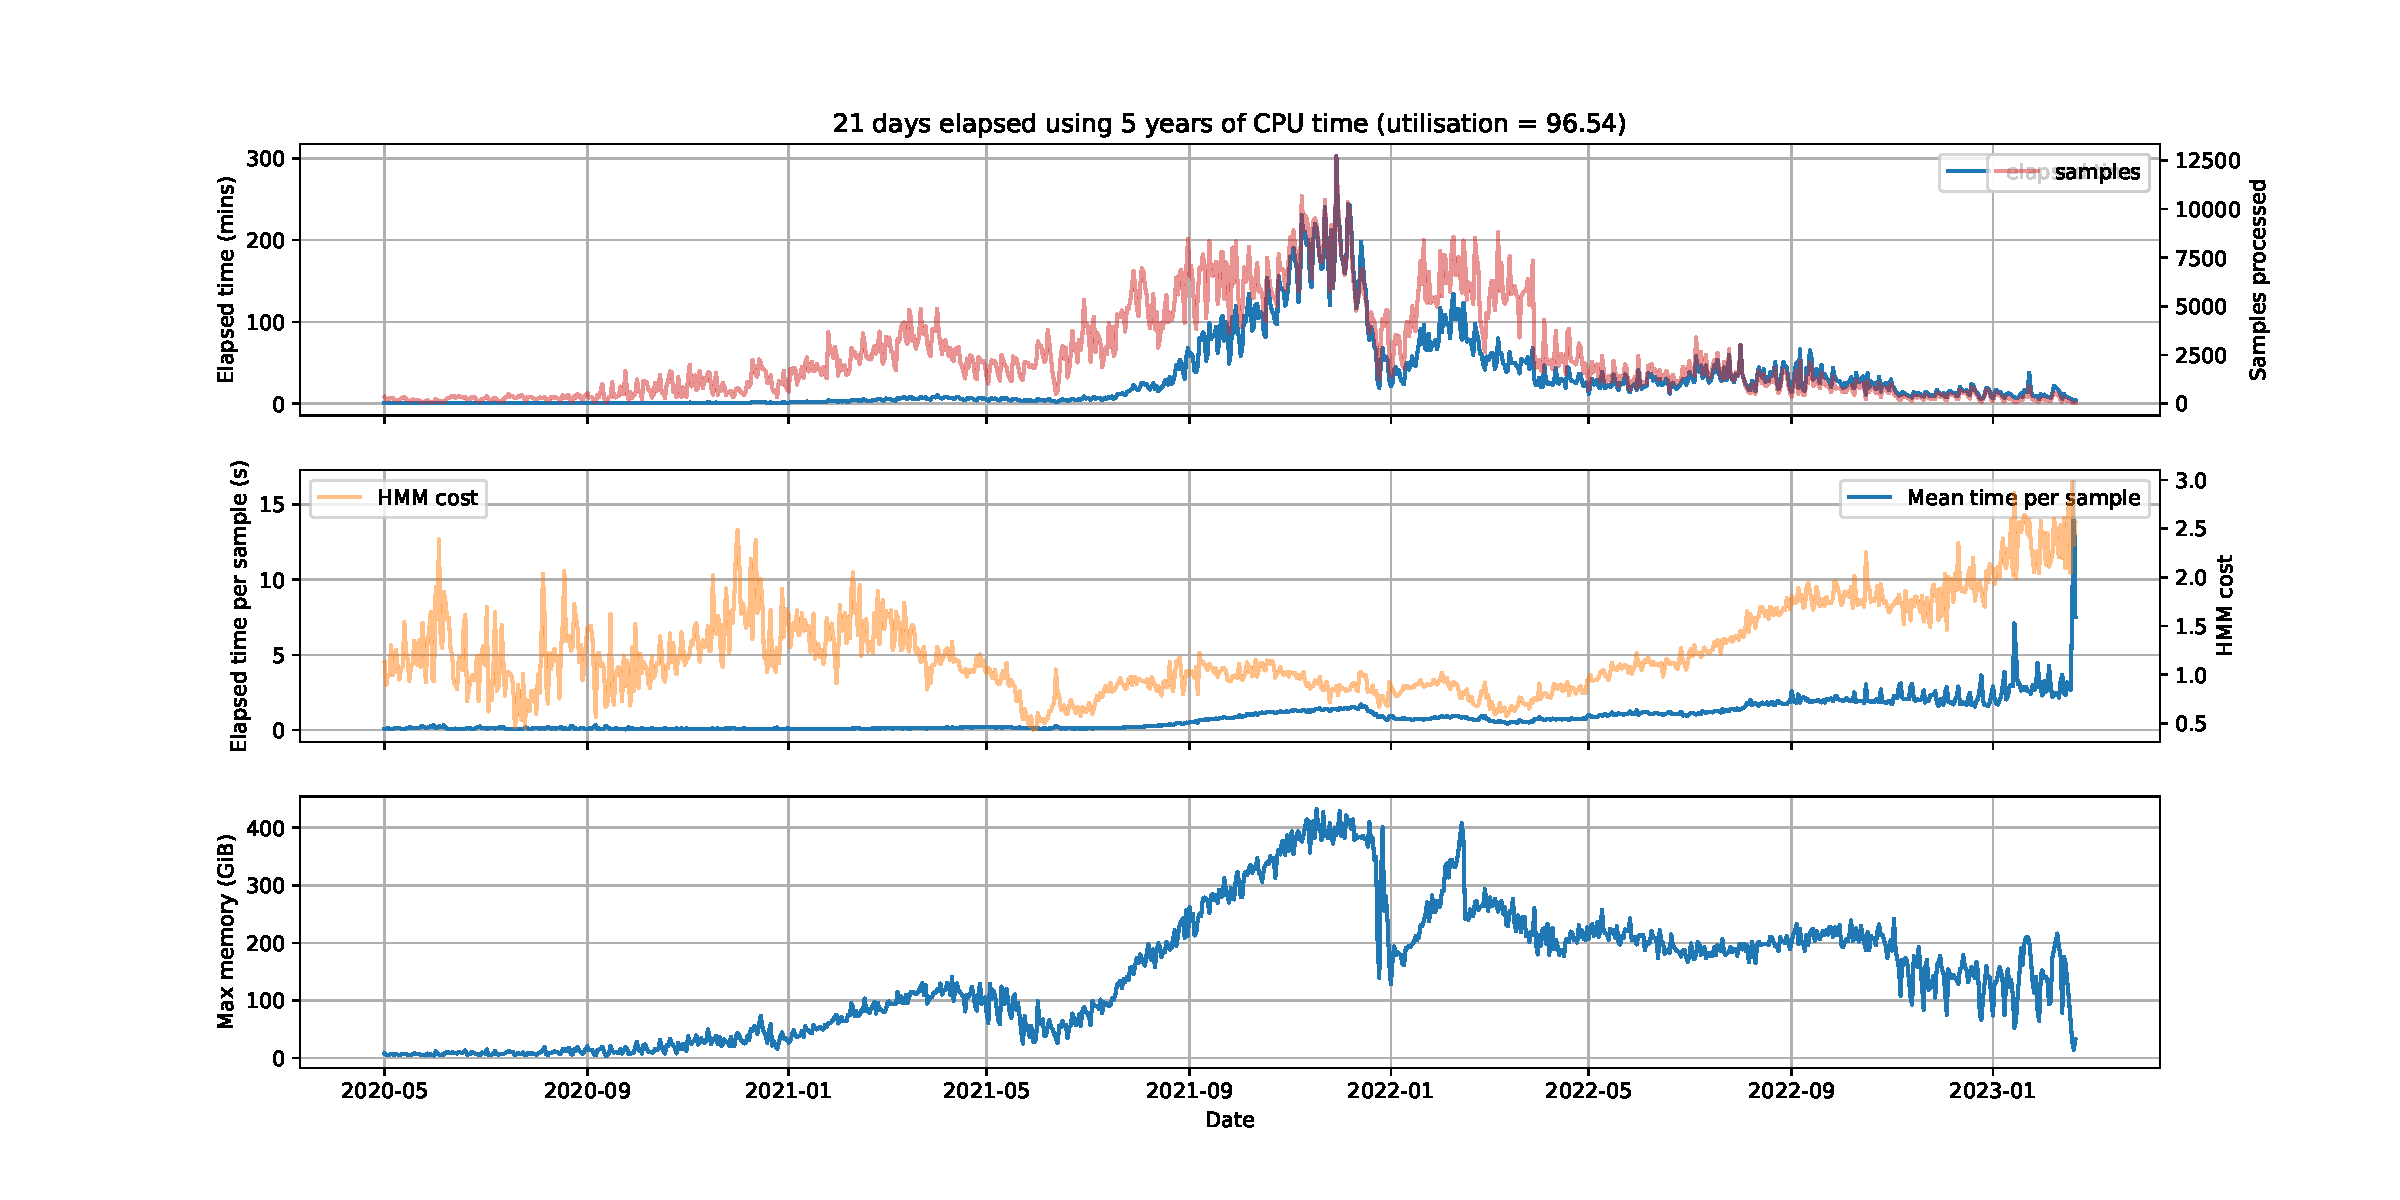
\includegraphics[width=\linewidth]{inference-resources}
\caption{TODO caption}
\label{fig:inference_resources}
\end{figure}


\begin{figure}
\centering
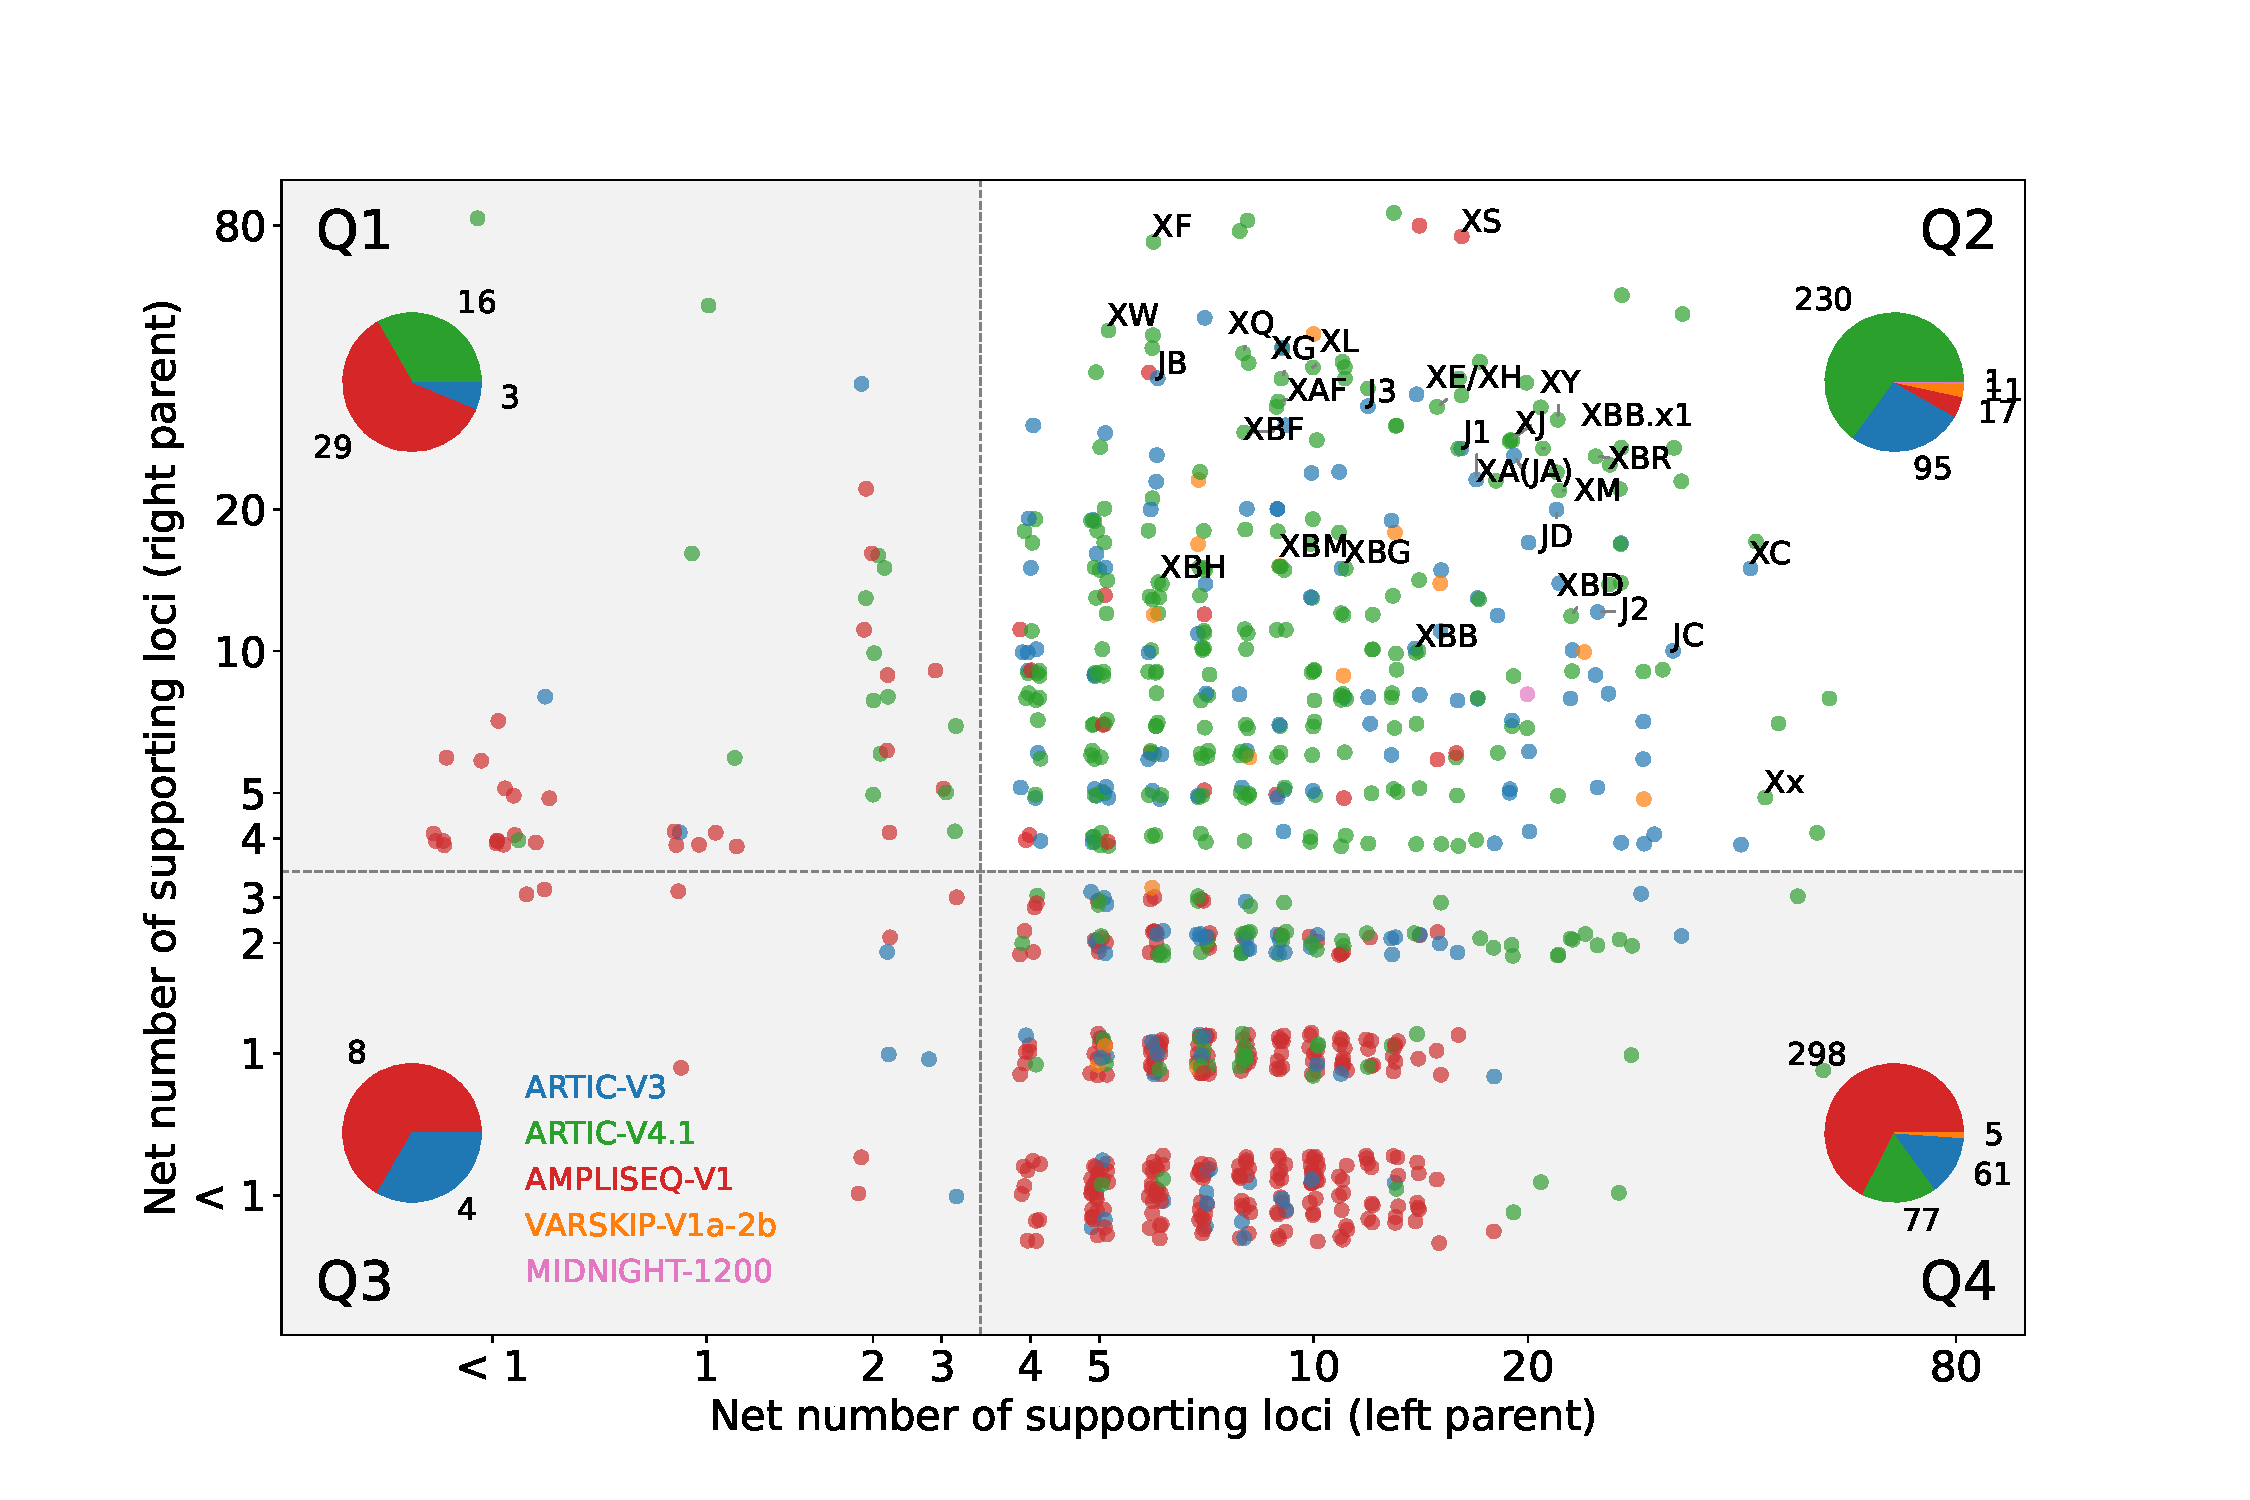
\includegraphics[width=\linewidth]{recombinant_qc}
\caption{
Quality control of recombination events.
Scatterplot of recombination events by the net number of supporting loci
on the left parent (x-axis) and the right parent (y-axis).
The shaded regions highlight artifactual recombination events,
which have fewer than 4 net supporting loci
on one side or both sides of the suggested breakpoint.
Colors indicate the primer scheme used for sequencing.
The pie charts show breakdowns of the recombination events
by primer scheme per quadrant (labeled Q1 to Q4).
Recombination events associated with
the origins of Pango X lineages are labeled.
}
\label{fig:recombinant_qc}
\end{figure}

\newcommand{\cprheight}{4.0em}


\begin{figure}
\centering
% NOTE the size of the second "m" column doesn't matter, but we have to fix the
% size in order for vertical centering to work :sigh:
% The layout here isn't ideal, but it's incredibly fiddly to get center
% alignment veritically with cells to work, so this is good enough.
\begin{tabularx}{0.85\textwidth}{>{\centering\arraybackslash}m{1cm}>{\arraybackslash}m{1cm}}
Q1 & 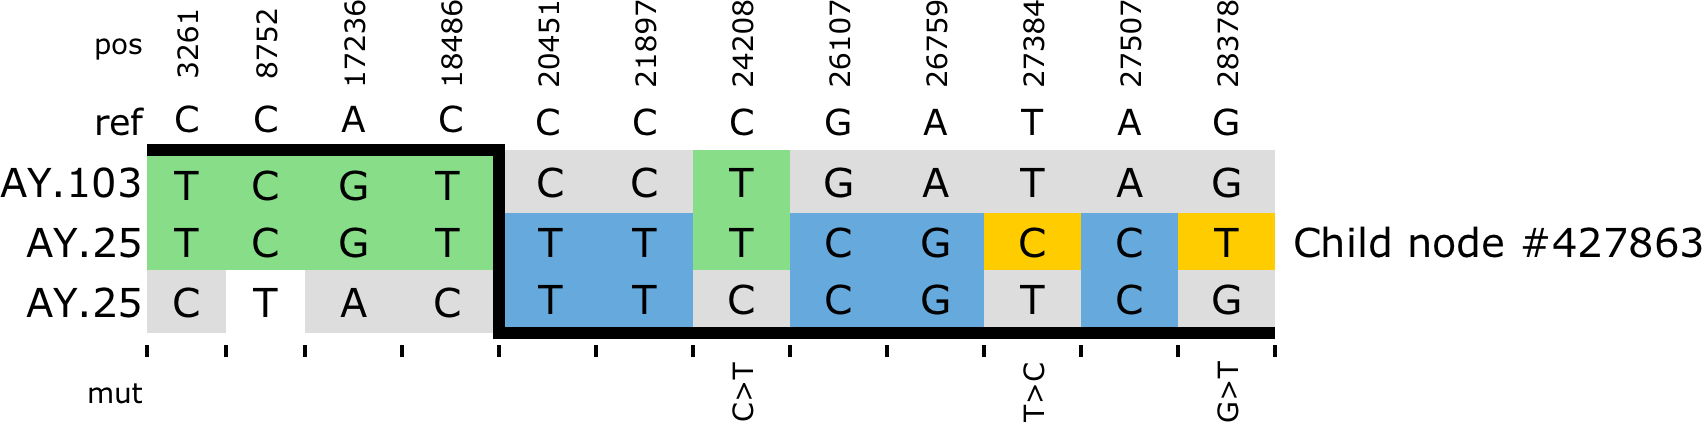
\includegraphics[height=\cprheight]{static/RE_node-QCpass-427863.png}\\
Q2 & 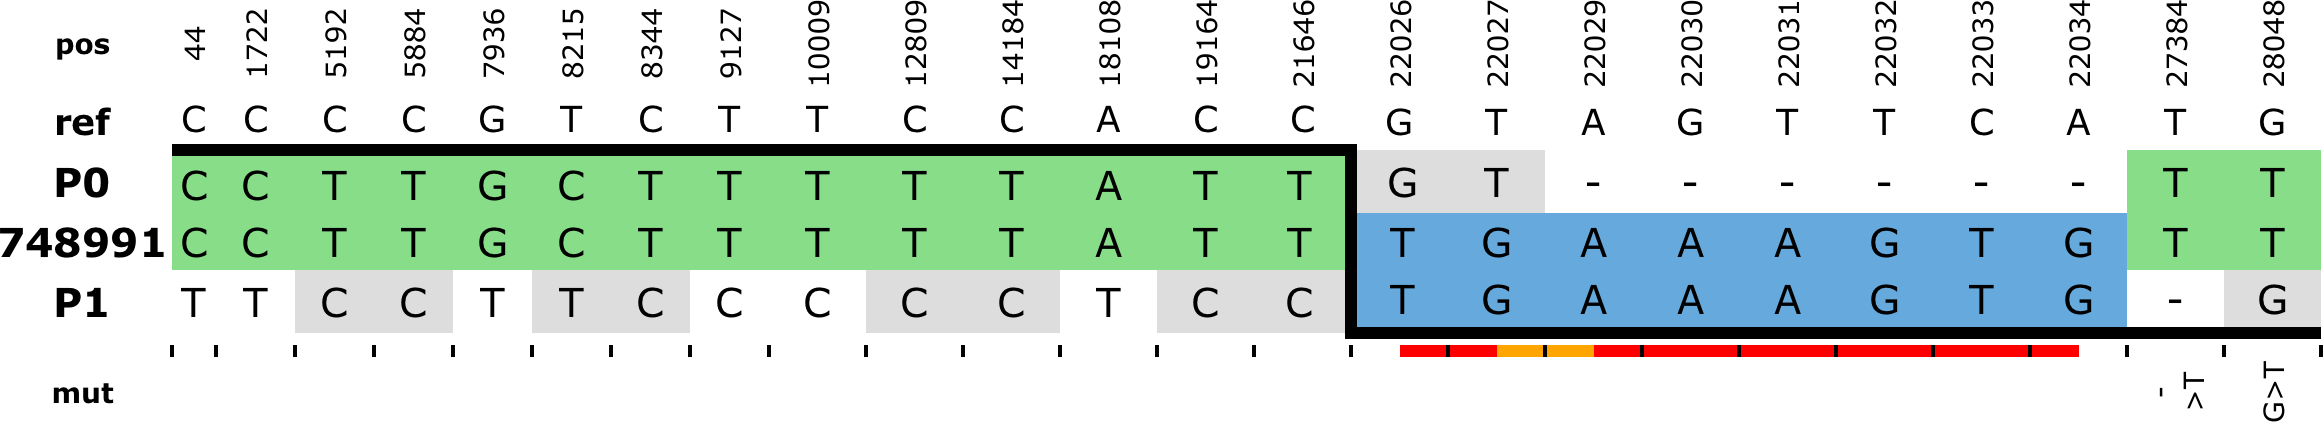
\includegraphics[height=\cprheight]{static/RE_node-QCfail-748991.png}\\
Q3 & 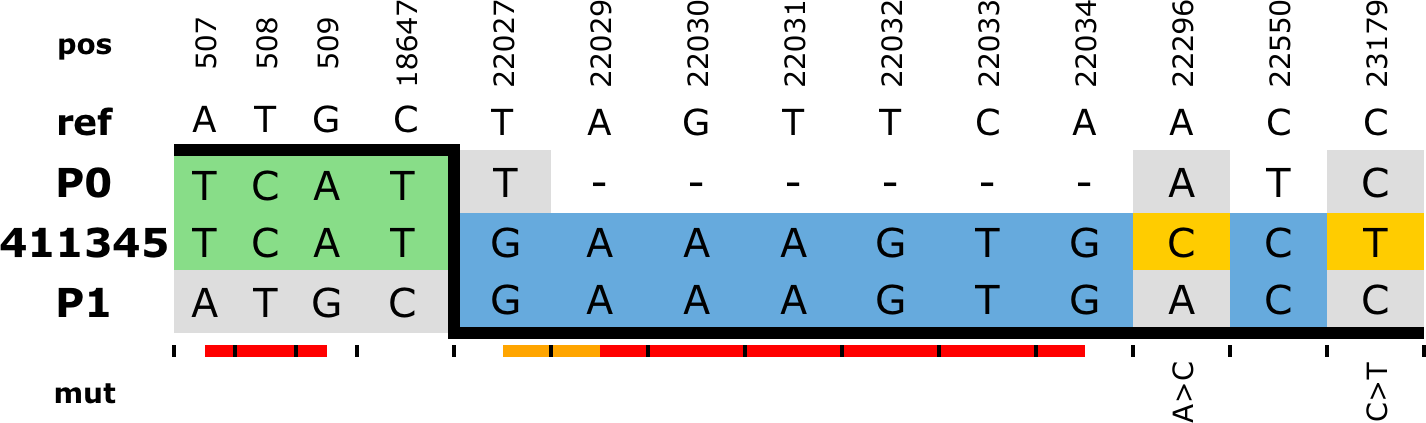
\includegraphics[height=\cprheight]{static/RE_node-QCfail-411345.png}\\
Q4 & 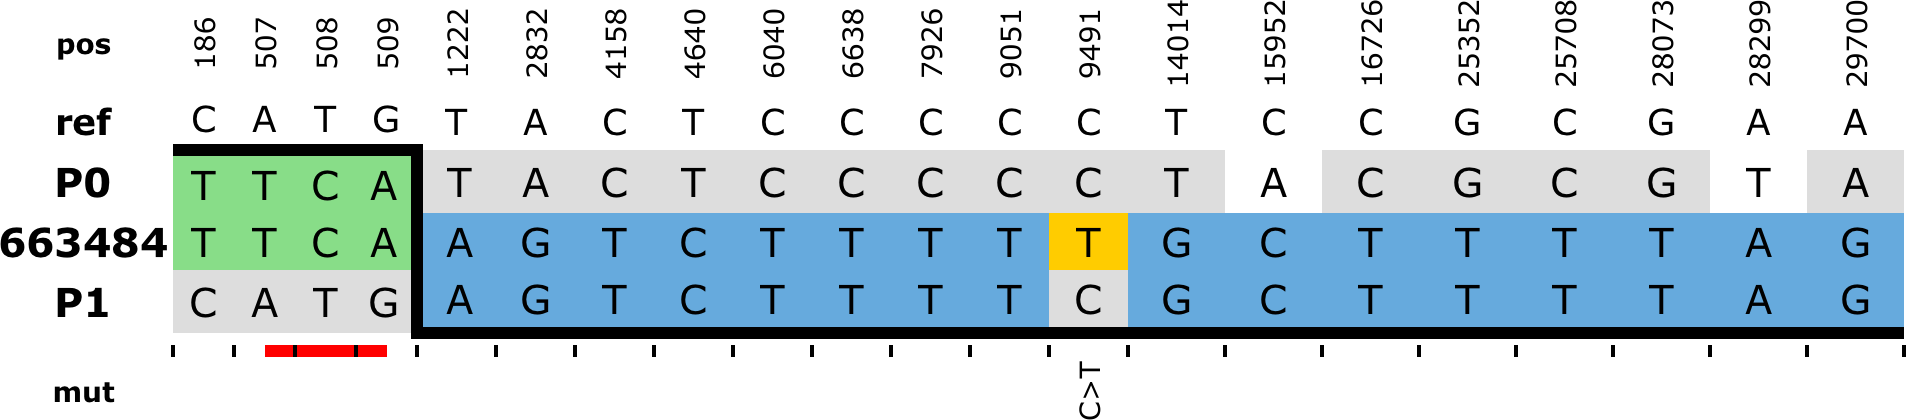
\includegraphics[height=\cprheight]{static/RE_node-QCfail-663484.png}\\
\end{tabularx}
\caption{
Illustrative copying patterns.
Q1 to Q4 are examples drawn from the labeled quadrants in Figure~\ref{fig:recombinant_qc}.
Q1 depicts the copying pattern of a recombination event that marginally passed QC,
whereas the others depict the copying patterns of recombination events that failed QC.
}
\label{fig:copying_pattern_examples}
\end{figure}


\renewcommand{\cprheight}{1.5em}
% Add some more space between rows. Note this it would be sligntly nicer if the 
% label was aligned vertically in the center of the row, but this is good
% enough for now.
\renewcommand{\arraystretch}{2}

\begin{figure}
\centering
\begin{tabularx}{\textwidth}{>{\centering\arraybackslash}m{1cm}>{\arraybackslash}m{1cm}}
XC & 
\includegraphics[height=\cprheight]{static/XC.png}\\
XBR & 
\includegraphics[height=\cprheight]{static/XBR.png}\\
XA & 
\includegraphics[height=\cprheight]{static/XA.png}\\
XS & 
\includegraphics[height=\cprheight]{static/XS.png}\\
XL & 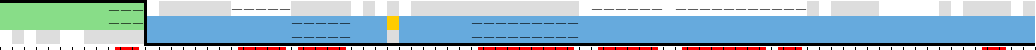
\includegraphics[height=\cprheight]{static/XL.png}\\
XBG &
\includegraphics[height=\cprheight]{static/XBG.png}\\
XBD & 
\includegraphics[height=\cprheight]{static/XBD.png}\\
XQ & 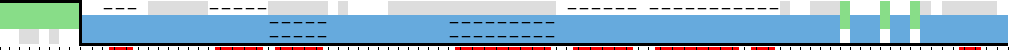
\includegraphics[height=\cprheight]{static/XQ++.png}\\
XBB & 
\includegraphics[height=\cprheight]{static/XBB.png}\\
XM & 
\includegraphics[height=\cprheight]{static/XM+XAL.png}\\
XBF & 
\includegraphics[height=\cprheight]{static/XBF.png}\\
XF & 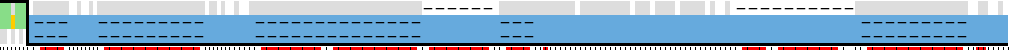
\includegraphics[height=\cprheight]{static/XF.png}\\
XY & 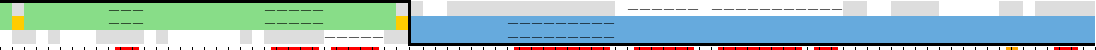
\includegraphics[height=\cprheight]{static/XY.png}\\
XG & 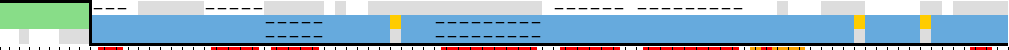
\includegraphics[height=\cprheight]{static/XG.png}\\
XW & 
\includegraphics[height=\cprheight]{static/XW.png}\\
Xx & 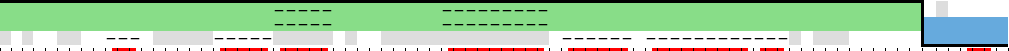
\includegraphics[height=\cprheight]{static/XZ++.png}\\
XE/XH  & 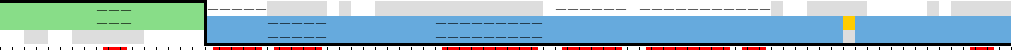
\includegraphics[height=\cprheight]{static/XE+XH.png}\\
XBH & 
\includegraphics[height=\cprheight]{static/XBH.png}\\
XBM & 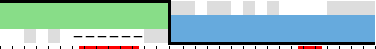
\includegraphics[height=\cprheight]{static/XBM.png}\\
XJ & 
\includegraphics[height=\cprheight]{static/XJ.png}\\
\end{tabularx}
\caption{Copying patterns for the 20 recombination events associated with Pango 
X lineages listed in Table~\ref{tab:pango_x_lineages} (in the same order)}
\label{fig:pango_x_copying_patterns}
\end{figure}

% Reset this in case we make any more tables beyond this
\renewcommand{\arraystretch}{1}


\begin{figure}
\centering
\centering
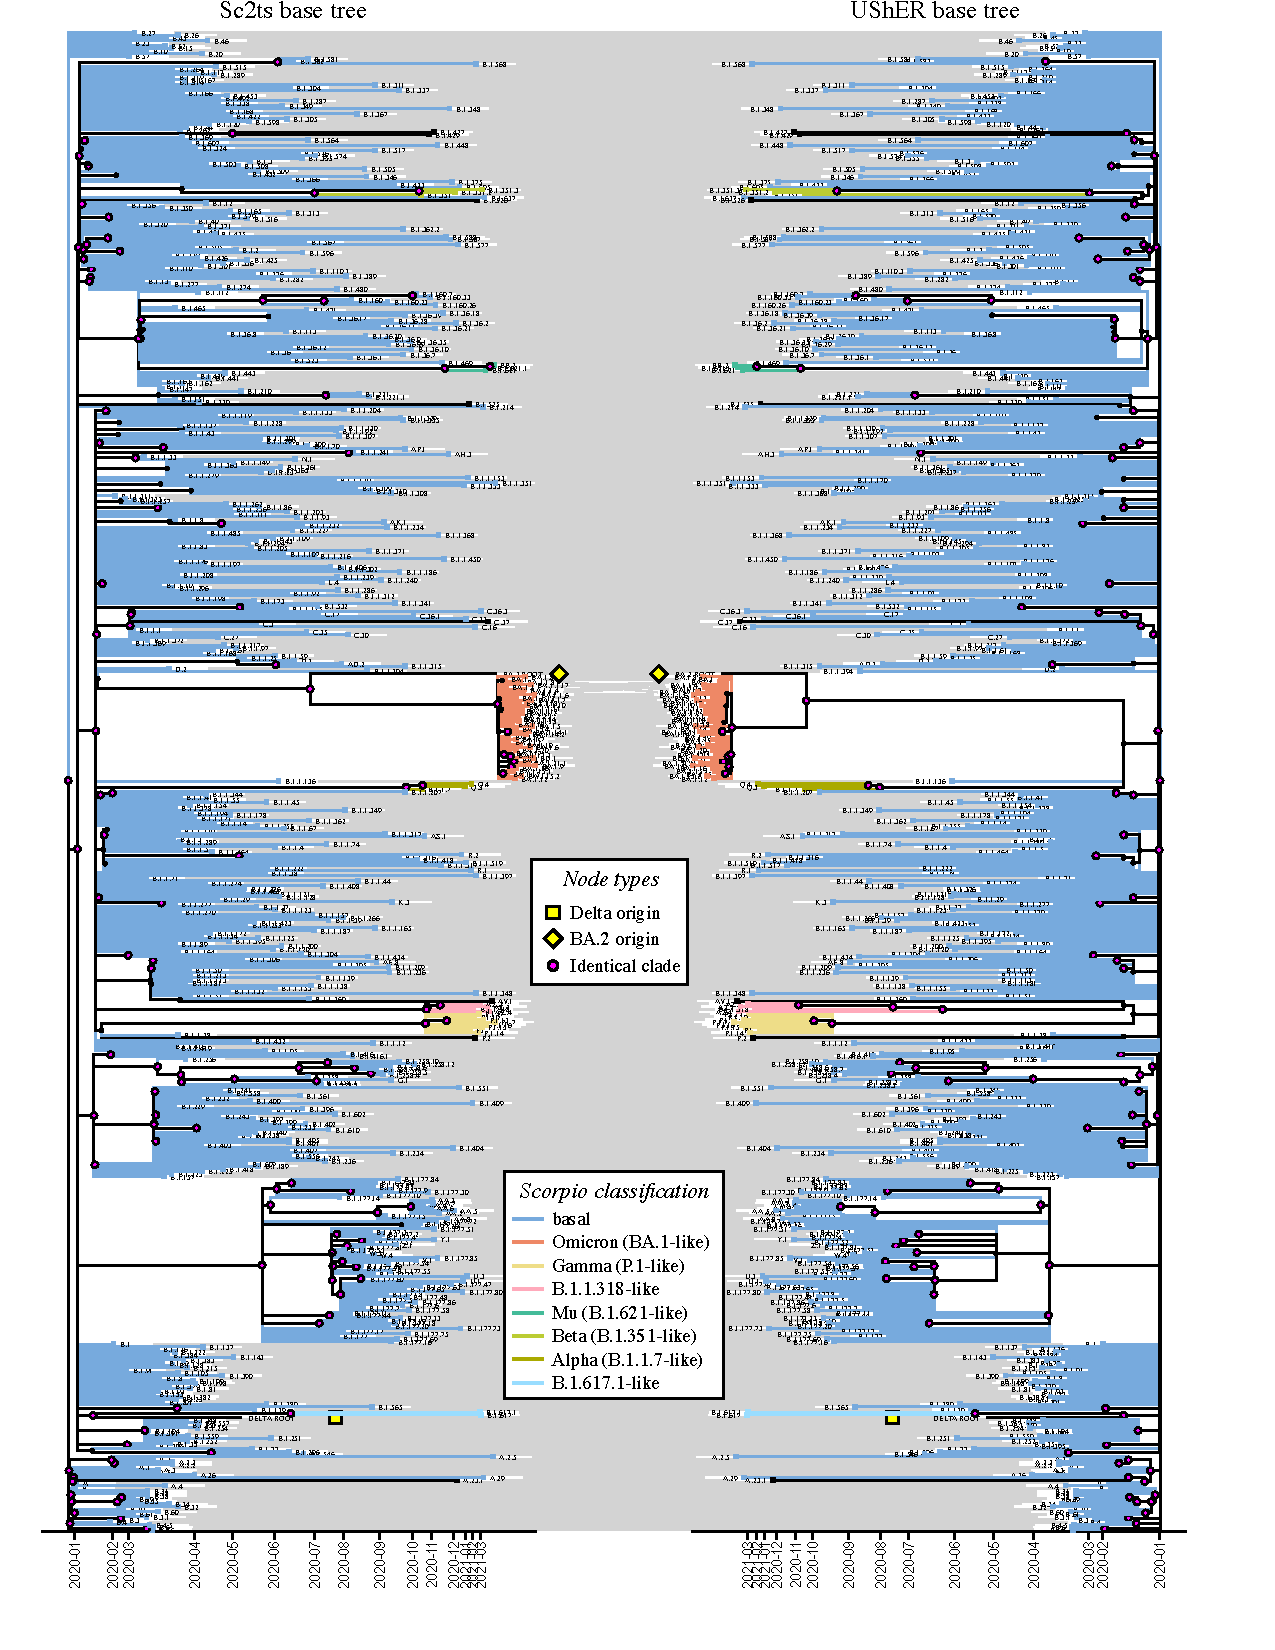
\includegraphics[width=\linewidth]{tanglegram_base_tree.pdf}
\caption{
Tanglegram comparing phylogenetic backbones of sc2ts and UShER.
}
\label{fig:tanglegram_base}
\end{figure}

\begin{figure}
\centering
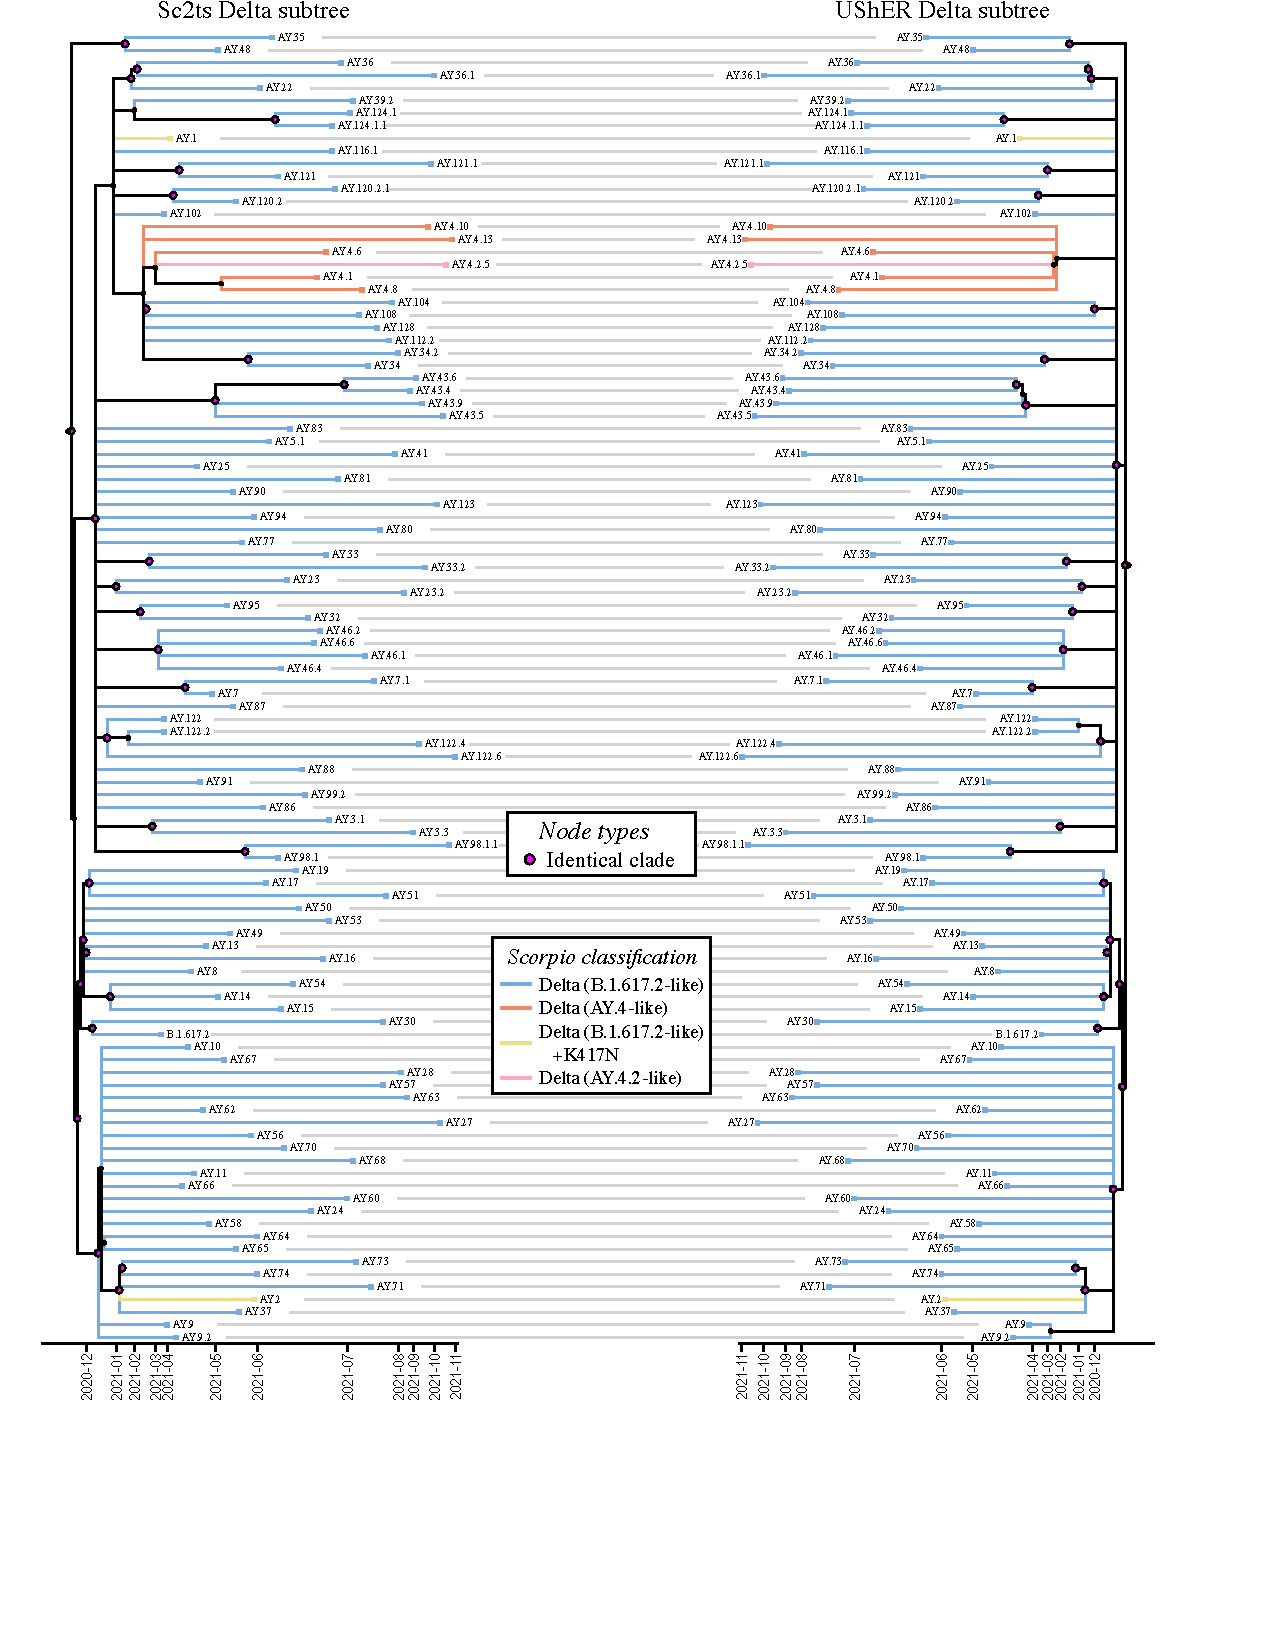
\includegraphics[width=\linewidth]{tanglegram_Delta_subtree.pdf}
\caption{
Tanglegram comparing sc2ts and UShER on the Delta subtree.
}
\label{fig:tanglegram_delta}
\end{figure}

\begin{figure}
\centering
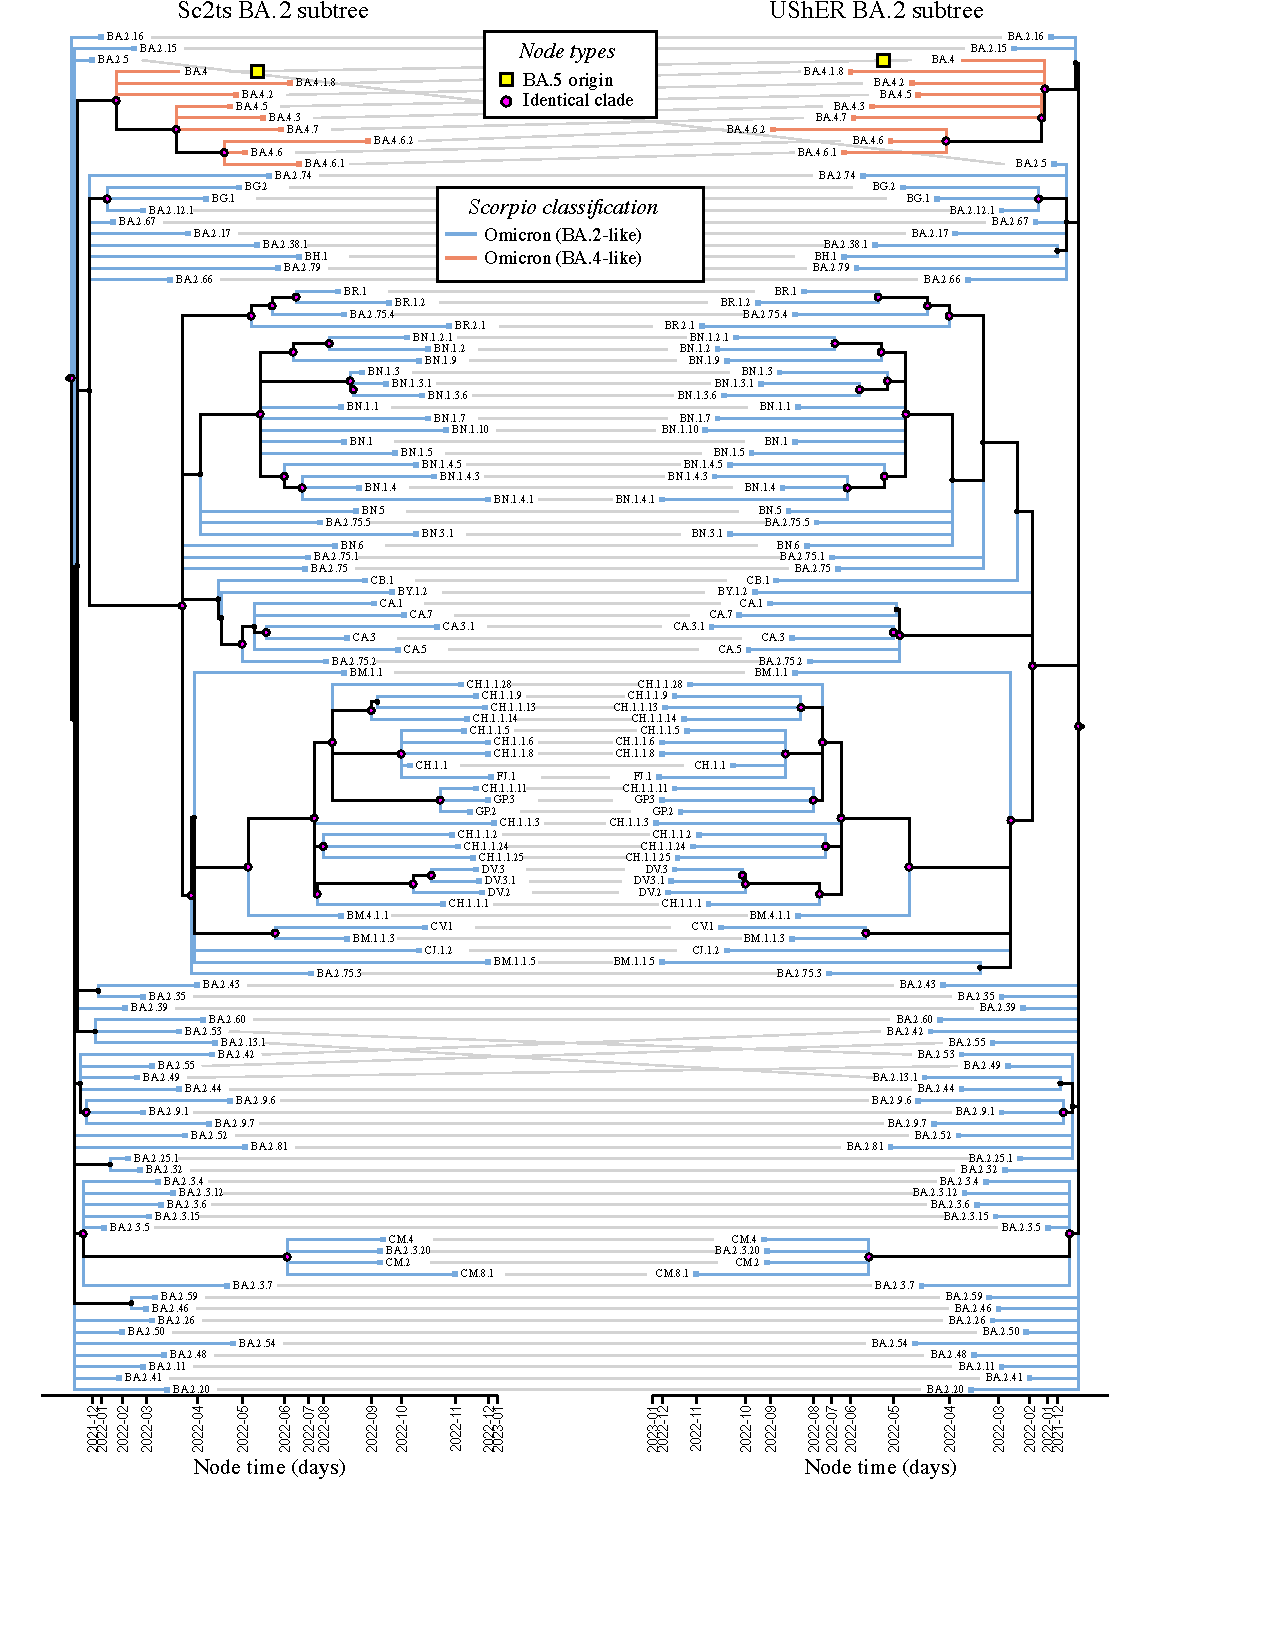
\includegraphics[width=\linewidth]{tanglegram_BA.2_subtree.pdf}
\caption{
Tanglegram comparing sc2ts and UShER on the BA.2 subtree.
}
\label{fig:tanglegram_ba2}
\end{figure}

\begin{figure}
\centering
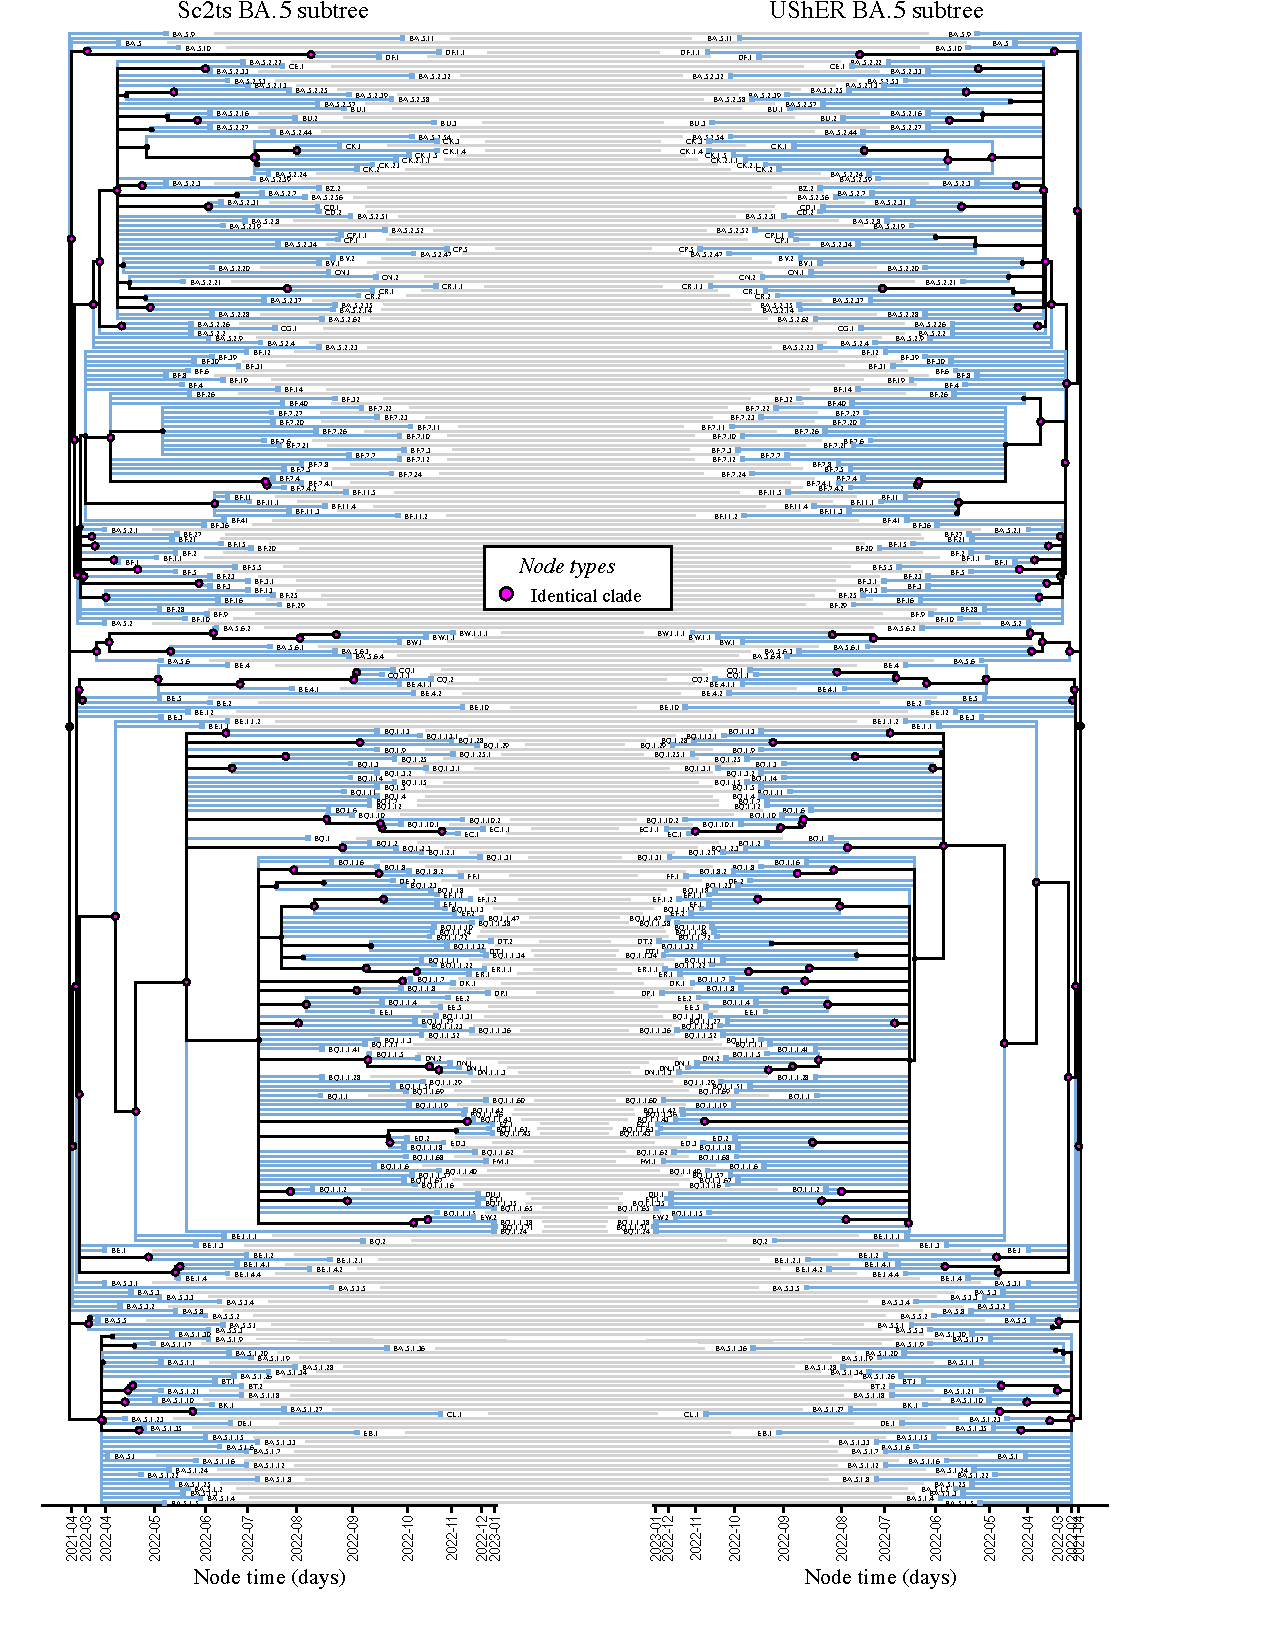
\includegraphics[width=\linewidth]{tanglegram_BA.5_subtree.pdf}
\caption{
Tanglegram comparing sc2ts and UShER on the BA.5 subtree.
}
\label{fig:tanglegram_ba5}
\end{figure}


\begin{figure}
\centering
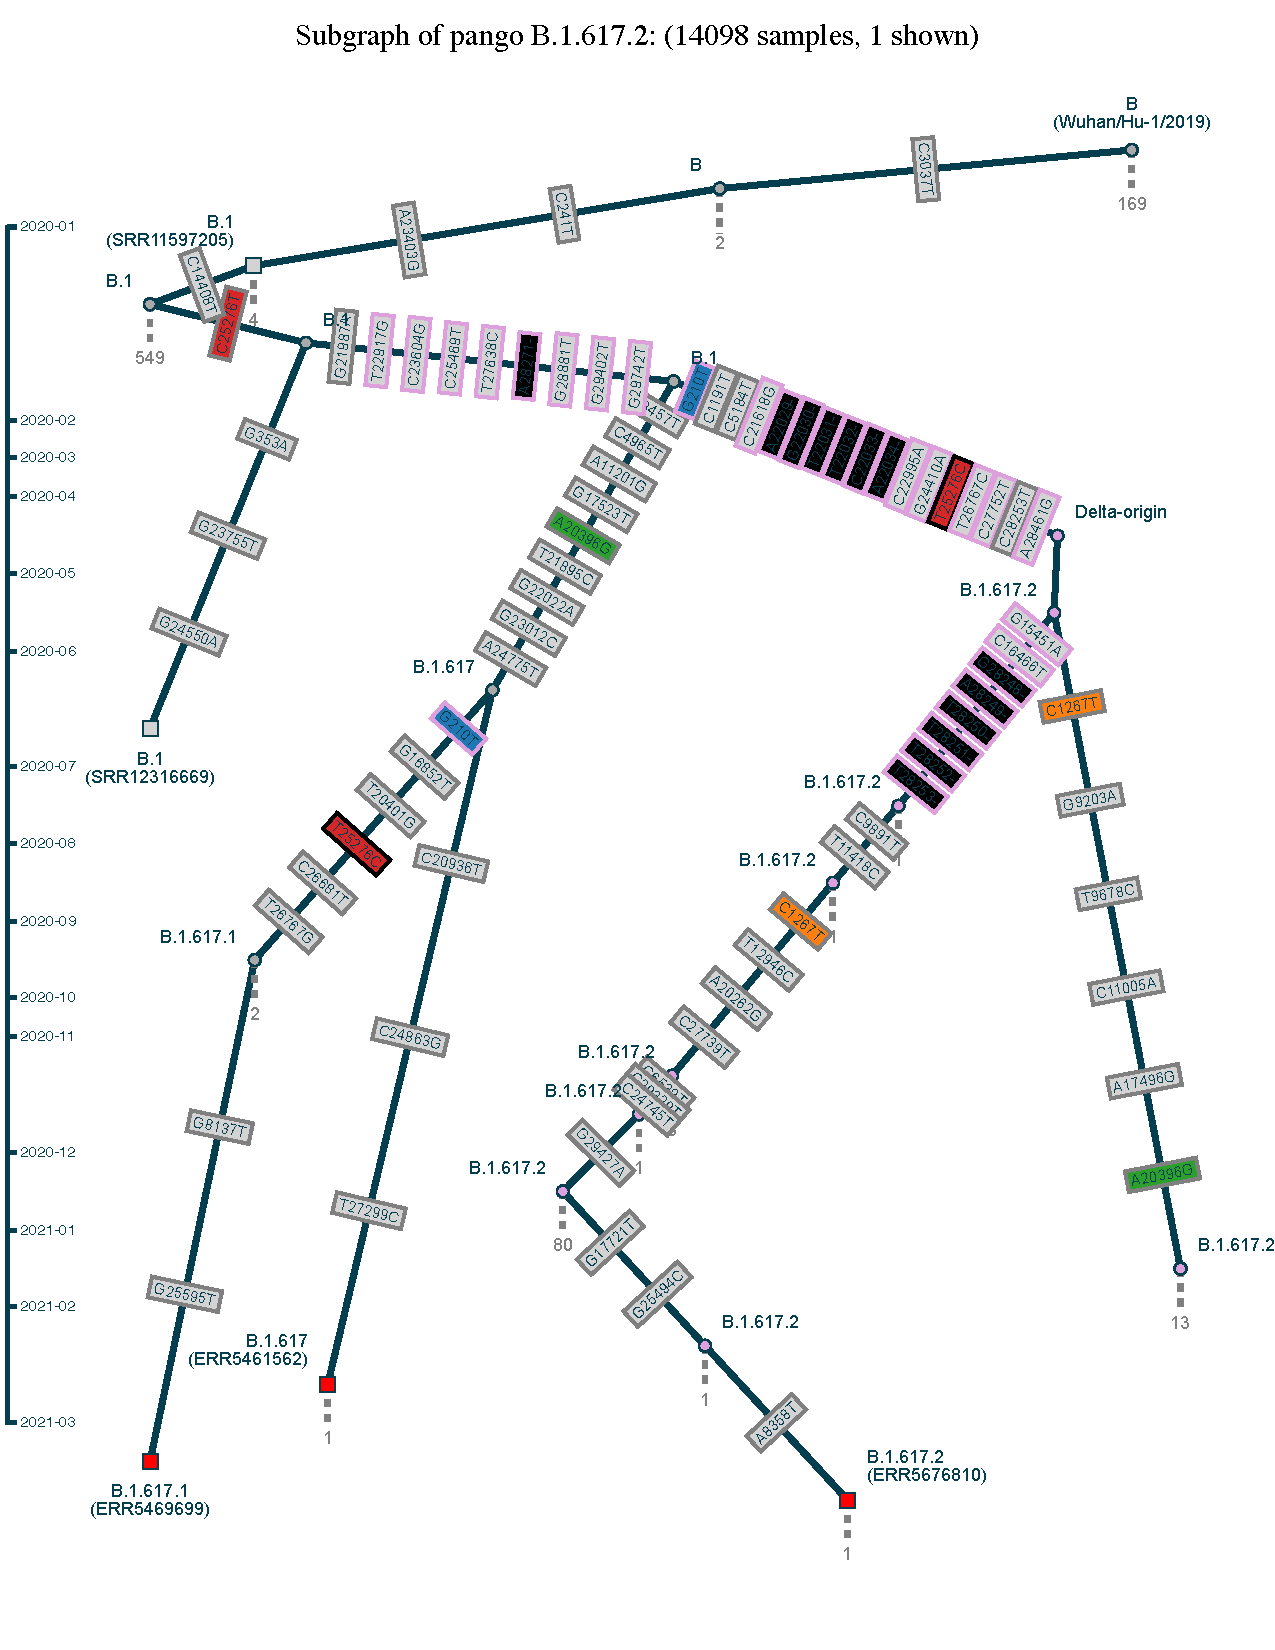
\includegraphics[width=0.85\linewidth]{subgraph-Alpha.pdf}
\caption{
Subgraph of Alpha. [Some notes to help the reader know this 
reflects known events]
}
\label{fig:subgraph_alpha}
\end{figure}

\begin{figure}
\centering
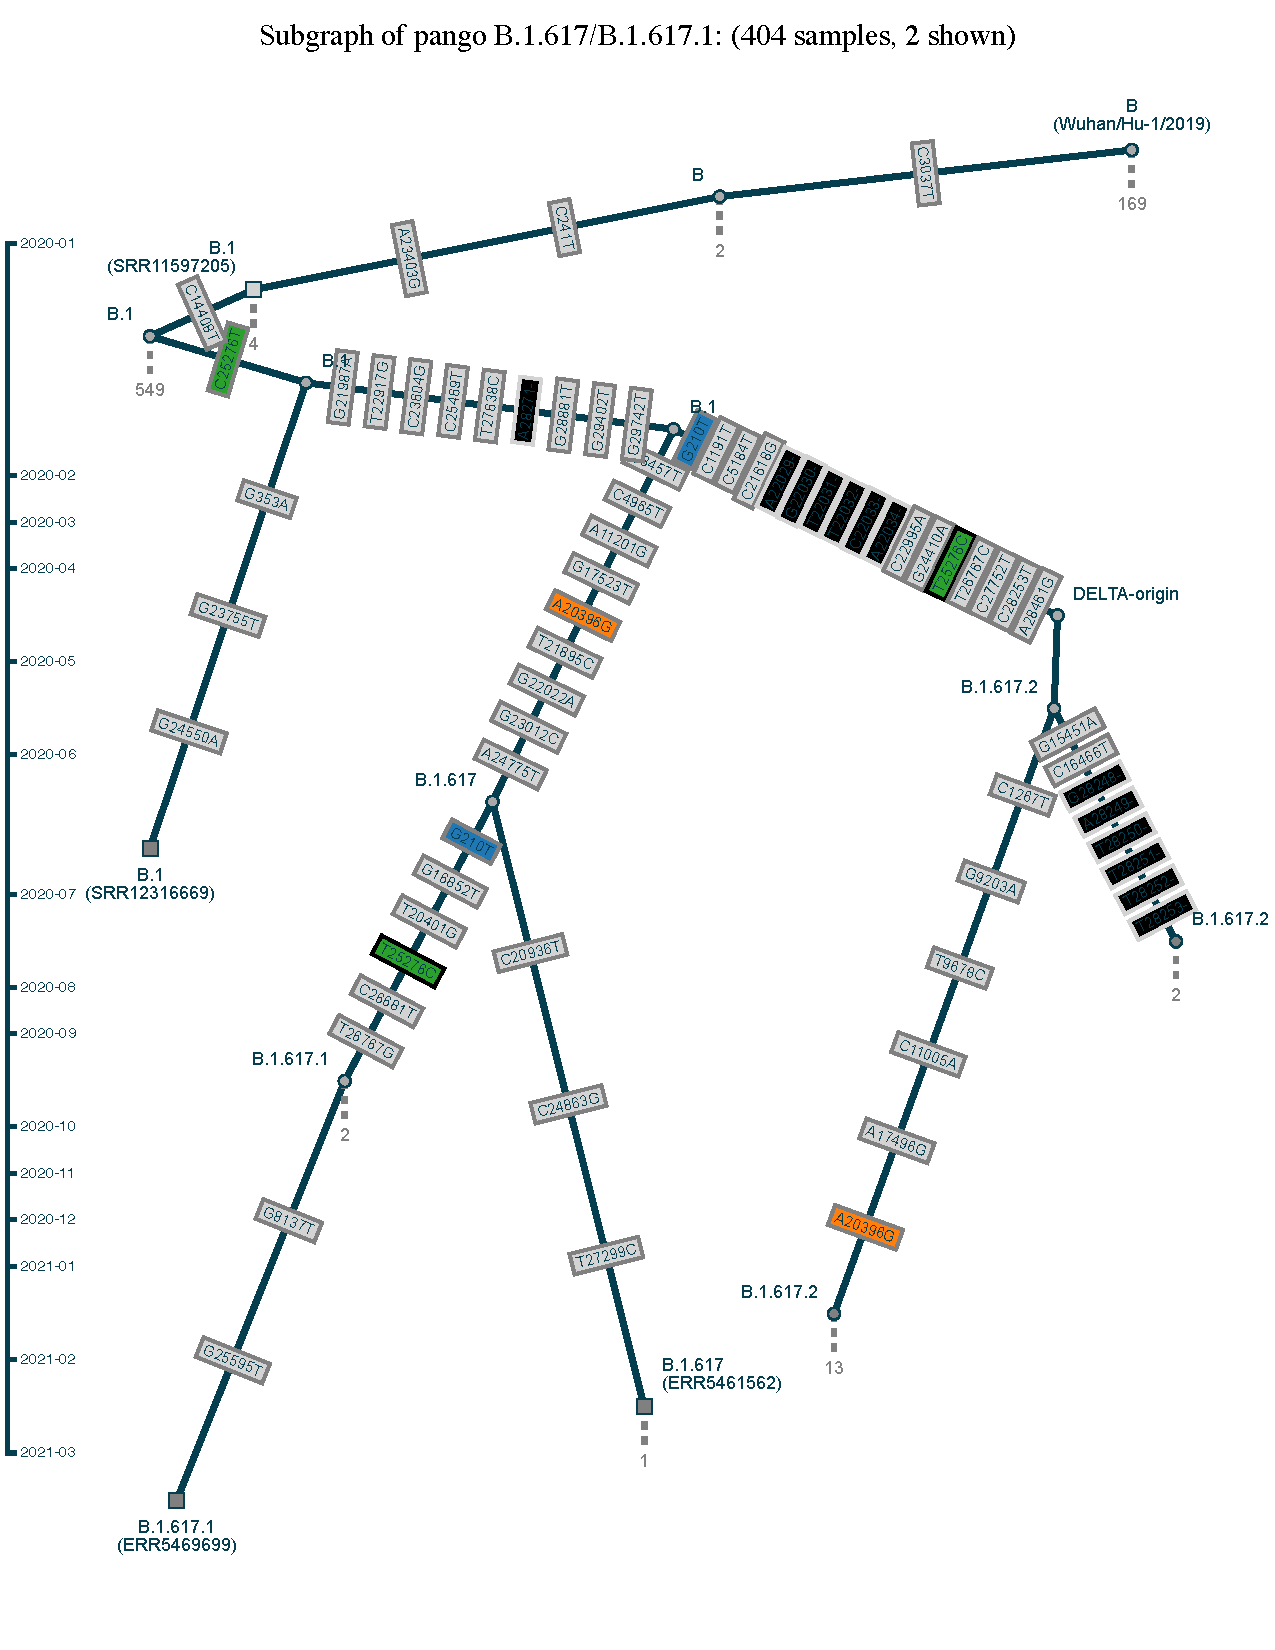
\includegraphics[width=0.85\linewidth]{subgraph-Delta.pdf}
\caption{
Subgraph of Delta. [Some notes to help the reader know this 
reflects known events]
}
\label{fig:subgraph_delta}
\end{figure}

\begin{figure}
\centering
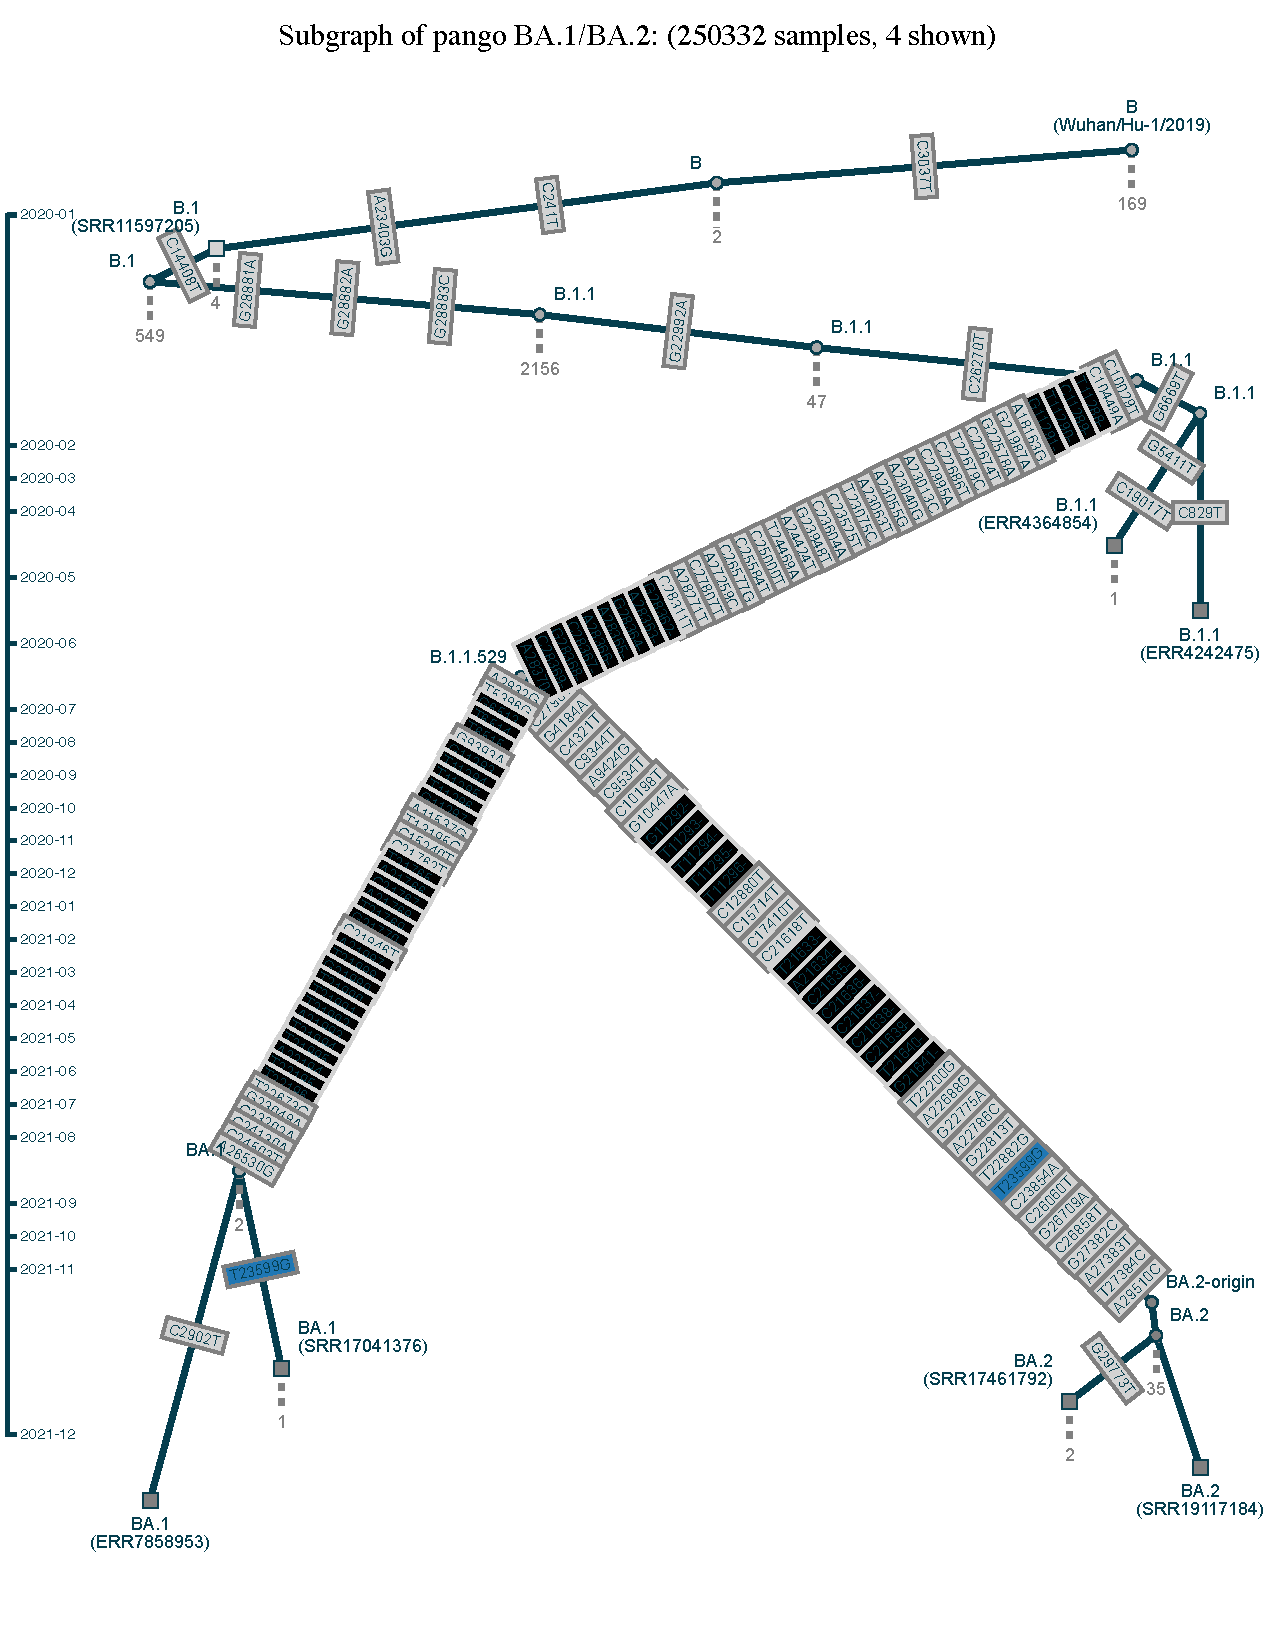
\includegraphics[width=0.85\linewidth]{subgraph-BA.1+BA.2.pdf}
\caption{
Subgraph of BA.1 and BA.2.
[Some notes to help the reader know this 
reflects known events]
}
\label{fig:subgraph_ba1_ba2}
\end{figure}


\begin{figure}
\centering
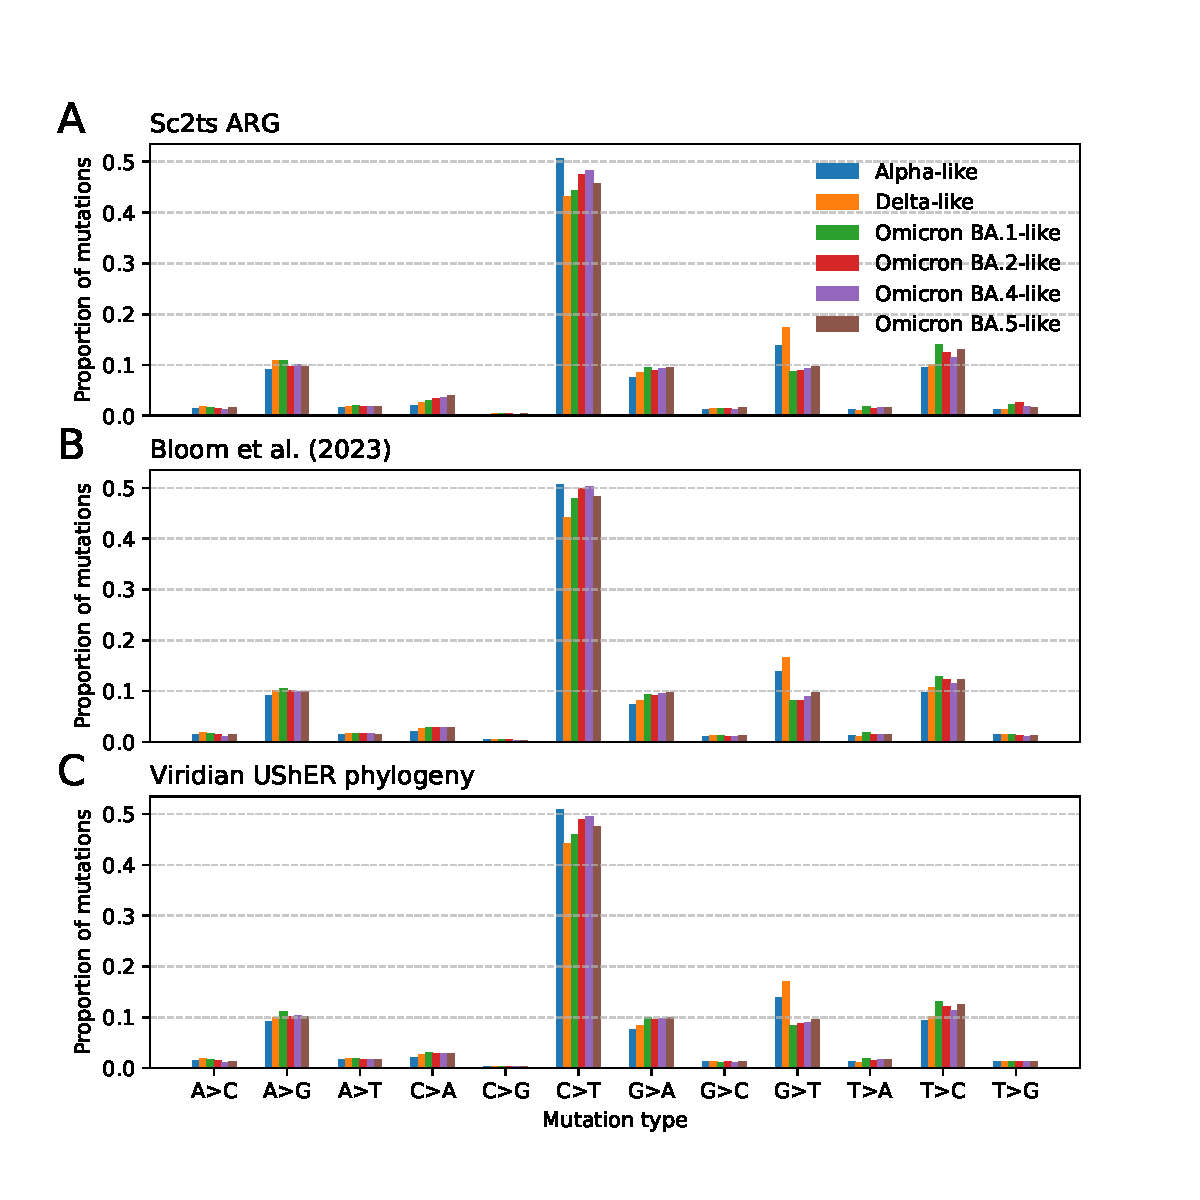
\includegraphics[width=\linewidth]{mutational_spectra}
\caption{
All-site mutational spectra of major VOCs calculated from the sc2ts ARG (A),
the mutation count data from Bloom et al. (2023)\cite{Bloom2023} (B), and
the Viridian UShER phylogeny from Hunt et al. (2024)\cite{Hunt2024}.
}
\label{fig:mutational_spectra}
\end{figure}


\begin{figure} 
\centering
\includegraphics[width=0.5\textwidth]{LS_model_schematic}
\caption{
A schematic of the Li and Stephens (LS)
model, in which a focal sequence (bottom) is described as an
imperfect mosaic of the sequences in a reference panel.
Black crosses along the focal sequence show sequencing
errors or mutations.
In the standard formulation, at site $\ell$, the recombination probability is $r_\ell$,
the mutation probability is $\mu_\ell$ and $n$
denotes the size of the reference panel.
The Viterbi algorithm can be used to find a
``copying path'' through the reference panel for a given focal sequence that
maximises the likelihood under these parameters. Unseen states in the reference panel are shown as colored lines enclosed by
the grey box. The black arrow describes the true path through the data which leads to the emitted
focal sequence below. Examples of transition and
emission probabilities along this trajectory are shown by the red and blue
arrows, respectively.
}
\label{fig:ls_diagram}
\end{figure}

\begin{figure}
\centering
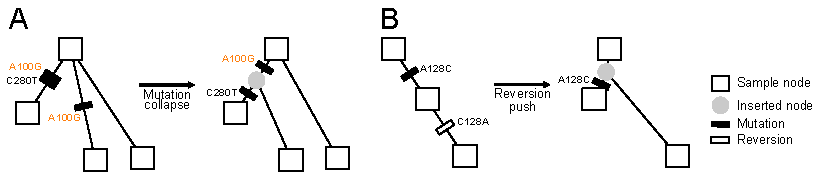
\includegraphics[width=0.85\linewidth]{tree_ops}
\caption{
Parsimony improving heuristics. (A) Mutation collapsing. Mutation A100G is
shared by two siblings, and we create a new node to represent the ancestor
on which this mutation occured. (B) Reversion pushing. Mutation A128C is
immediately reverted by C128A, and we create a new node to represent the 
ancestor that did not carry A128C.
}
\label{fig:parsimony_ops}
\end{figure}


\end{document}
